\documentclass[10pt,a4paper]{book}
\usepackage[utf8x]{inputenc}

\usepackage{amsmath}
\usepackage{amsfonts}
\usepackage{amssymb}
\usepackage{amsthm}


\usepackage[top=2.3cm, bottom=2.3cm, left=3cm, right=3cm]{geometry}
%\parskip=5mm
\usepackage{lmodern}
\usepackage{enumerate}
\usepackage{appendix}
\usepackage{mathtools}
\usepackage{braket}
\usepackage{graphicx}
\usepackage{fancyhdr} % activamos el paquete
\usepackage{subcaption}  % use for side-by-side figures
\usepackage[hidelinks]{hyperref}   
\usepackage{xcolor}
\hypersetup{colorlinks,
	linkcolor={red},
	citecolor={green},
	urlcolor={blue}}
   % external documents and URLs
\usepackage{units}
\usepackage{url}
\usepackage{fancybox}
\usepackage{amssymb}
\usepackage{multirow}
\usepackage{float}
\usepackage{bigints}
\usepackage{array}
\setlength{\parskip}{\baselineskip}
\numberwithin{equation}{chapter}
\numberwithin{figure}{chapter}
\numberwithin{table}{chapter}

\newtheorem{theorem}{Theorem}[section]
\newtheorem{corollary}{Corollary}
\newtheorem{lemma}{Lemma}[section]
\newtheorem*{remark}{Remark}
\newtheorem{prop}{Proposition}[section]
\setlength{\parskip}{-0.1mm}


\begin{document}
\frontmatter % Use roman page numbering style (i, ii, iii, iv...) for the pre-content pages

\pagestyle{plain} % Default to the plain heading style until the thesis style is called for the body content

\begin{titlepage}

\begin{center}

\vspace*{.02\textheight}
{\scshape\LARGE \href{https://www.uibk.ac.at/}{Leopold-Franzens-Universit{\"a}t Innsbruck}\par}\vspace{1.0cm} % University name
\textsc{\Large Master Thesis}\\[0.5cm] % Thesis type
\hline \\[0.4cm] % Horizontal line
{\huge \bfseries Efficient Two Dimensional Quantum Repeater \par}\vspace{0.4cm} % Thesis title
\hline \\[1.5cm] % Horizontal line
 
\begin{minipage}[t]{0.4\textwidth}
\begin{flushleft} \large
\emph{Author:}\\
\href{https://www.uibk.ac.at/th-physik/staff/lopez-bravo/}{Sonia \textsc{López-Bravo}} % Author name - remove the \href bracket to remove the link
\end{flushleft}
\end{minipage}
\begin{minipage}[t]{0.4\textwidth}
\begin{flushright} \large
\emph{Supervisor:} \\
\href{https://www.uibk.ac.at/th-physik/staff/duer/}{Prof. Mag. Dr.\ Wolfgang \textsc{Dür}} % Supervisor name - remove the \href bracket to remove the link  
\end{flushright}
\end{minipage}\\[2cm]
 \large \textit{A thesis submitted in partial fulfillment of the requirements\\ for the degree of Master of Science}\\[0.3cm] % University requirement text
\textit{in the}\\[0.4cm]
\href{https://www.uibk.ac.at/th-physik/research/quanteninformation/}{Leopold-Franzens-Universit{\"a}t Innsbruck}\\ at \href{https://www.uibk.ac.at/th-physik/}{Institut f{\"u}r Theoretische Physik}\\[1cm] % Research group name and department name


\includegraphics[scale=0.8]{UIBK.jpg}\\[1cm] % University/department logo - uncomment to place it
{\large \today}\\[4cm] % Date

\end{center}
\end{titlepage}


\begin{declaration}
\addchaptertocentry{\authorshipname} % Add the declaration to the table of contents

\noindent\textbf{Leopold-Franzens-Universit{\"a}t Innsbruck}\\

\noindent Ich erkl{\"a}re hiermit an Eides statt durch meine eigenh{\"a}ndige Unterschrift, dass ich die vorliegende Arbeit selbst{\"a}ndig verfasst und keine anderen als die angegebenen Quellen und Hilfsmittel verwendet habe. Alle Stellen, die w{\"o}rtlich oder inhaltlich den angegebenen Quellen entnommen wurden, sind als solche kenntlich gemacht.\\
Die vorliegende Arbeit wurde bisher in gleicher oder {\"a}hnlicher Form noch nicht als Magister-/Master-/Diplomarbeit/Dissertation eingereicht. \\
 
\noindent Unterschrift:\\
\rule[0.5em]{25em}{0.5pt} % This prints a line for the signature
 
\noindent Datum:\\
\rule[0.5em]{25em}{0.5pt} % This prints a line to write the date
\end{declaration}

\cleardoublepage

%----------------------------------------------------------------------------------------
%	QUOTATION PAGE
%----------------------------------------------------------------------------------------

\vspace*{0.2\textheight}
\begin{flushright}
\noindent\enquote{\itshape I was within and without, 

simultaneously enchanted and repelled by the inexhaustible variety of life. }\bigbreak
\end{flushright}
\hfill Fitzgerald, F. Scott \textit{The Great Gatsby}

%----------------------------------------------------------------------------------------
%	ABSTRACT PAGE
%----------------------------------------------------------------------------------------

\newenvironment{abstract}%
    {\cleardoublepage\thispagestyle{empty}\null\vfill\begin{center}%
    \bfseries Abstract \end{center}}%
    {\vfill\null}
\begin{abstract}
Long-distance quantum communication is one of the most appealing applications of quantum technology. It
promises secure classical communication via quantum key distribution and is also essential for distributed quantum computation. High-rate quantum communication over long distances is possible using quantum repeaters, which either utilize quantum error correction or combine entanglement purification and entanglement swapping. In a real-world application of quantum communication one needs flexible multi-user structures that allow for quantum communication between arbitrary pairs of parties and facilitate also multi-user applications. Sharing of multi-partite entangled states between parties offers a solution, allowing for parallel quantum communication. To address this problem, a 2D quantum repeater architecture was proposed in \cite{twodim} to establish long-distance entanglement shared between multiple partners. The scheme was based on the creation of self-similar multi-qubit entanglement structures at growing scale, where variants of entanglement swapping and multi-party entanglement purification are combined to create high fidelity entangled states. Here we propose an efficient 2D quantum repeater based on four-particle GHZ states, which allows quantum error correction against single qubit errors but also against multi-qubit errors. 
\end{abstract}
%----------------------------------------------------------------------------------------
%	ACKNOWLEDGEMENTS
%----------------------------------------------------------------------------------------

\newenvironment{acknowledgements}%
    {\cleardoublepage\thispagestyle{empty}\null\vfill\begin{center}%
    \bfseries Acknowledgements\end{center}}%
    {\vfill\null}
    \begin{acknowledgements}
        These are the acknowledgements.
        \end{acknowledgements}

\tableofcontents


\mainmatter % Begin numeric (1,2,3...) page numbering

\pagestyle{thesis}


\chapter{Introduction}

In the year 1935, Einstein, Podolsky and Rosen expressed their concerns about quantum mechanics as an incomplete theory \cite{EPR}. They recognized a "spooky" feature which implied the existence of global states of a composite system which cannot be written as a product of the states of individual subsystems.
They proposed a Gedanken experiment, known as EPR paradox, which should prove that description of quantum mechanics was incomplete and there were fixed values of physical quantities prior to measurement, known as hidden variables. This phenomenon, today known as “entanglement,” was originally called by Schrödinger “Verschränkung” in the same year and he formulated some of the mathematical implications of entanglement on the statistics of measurement outcomes \cite{schrodinger}. 

In 1964 Bell accepted the EPR conclusion - that quantum description of reality was not complete- as a working hypothesis and formalized the EPR idea of deterministic world in terms of local hidden variable model (LHVM) \cite{bell}. He assumes: (i) Realism, i.e. measurement results are determined by properties the particles carry prior to, and independent of, measurements; (ii) Locality, i.e. results obtained at one localition are independent of any action performed spacelike separated; and (iii) Freedom, i.e. the setting is independent of the hidden variables which determine the local results. Bell's theorem states that any physical theory that incorporates local realism impose constrains in the form of inequalities on statistical correlations in experiments involving bipartite systems. He showed that outcomes obtained from some entangled quantum state violate the Bell inequality, i.e local realism cannot reproduce all the predictions of quantum mechanics. It was not until 1981 when Aspect \textit{et al} reproduced a convincing test of violation of Bell inequalities \cite{aspect} using photons and demonstrated that predictions of quantum mechanics are correct, and since then many experiments have been tested LHVM leading to a evidence of violation of Bell's inequality. Nevertheless, Bell's theorem experiments rely on additional assumptions that open loopholes for local realism, and for that reason loophole-free Bell tests are performed \cite{belltest}, probably the most known is the recent Big Bell Test Collaboration \cite{bigbelltest}.

Entanglement plays a central role in some key discoveries such as quantum cryptography \cite{crypto}, quantum dense coding \cite{densecoding} and quantum teleportation \cite{teleportation}. Quantum entanglement inspired the idea of quantum computation, and it plays a central role in one-way quantum computing, measurement-based schemes and linear optics quantum computing. Entanglement also leaded to a new domain called quantum information, which comprises quantum communication, quantum error correction, quantum key distribution or entanglement purification.

It is clear that entanglement is a valuable resource for tasks that cannot be performed by means of classical resources. It can be manipulated, broadcasted, controlled and distributed. It can help in tasks as reduction of classical communication complexity, clock synchronization, super-radiance, superconductivity or quantum phase transitions. Unfortunately, quantum entanglement has three disagreeable but interesting features: It has in general a very complex structure, it is fragile with respect to enviroment, and it cannot be increased on average when systems are not in direct contact but distributed in spatially separated regions.

In the context of applications in quantum information theory, we may choose multipartite entanglement states rather than bipartite. We could use only bipartite entanglement but in experiments the dimension of Hilbert spaces is finite because we cannot store infinite qubits. The dimension of Hilbert spaces is indeed restricted in quantum networks and quantum technologies. Graph states form a rich class of entangled states that exhibit key aspects of multipartite entanglement. The general form of graph states has been introduced by Raussendorf \textit{et al} \cite{graph} as a generalization of cluster states \cite{cluster}. They have a variety of applications, most prominently as algorithmic resources of the one-way quantum computer, but also in other fields such as quantum error correction and multi-partite quantum communication. 

\section{Outline}
This work is structured as follows. In \autoref{chap:Graphs} we will introduce the concept of graph \cite{Diestel} and basic definitions regarding the features of graphs -most of them are intuitive- including how to manipulate graphs easily. We will see the notion of partitions and bipartite graphs which are crucial when modelling relations between two different classes of objects, as well as the notion of graph colouring. We will explain the operation of local complementation which is a very important graph operation in the context of equivalence classes of graphs and graph states, and the operation of vertex deletion which is related with the vertex-minor problem, with complexity $\mathbb{NP}$-complete. Finally, we will see how graphs are associated with quantum systems.

Once we are familiar with graphs and graph theory, we will see how they can be used in quantum theory of entanglement. In \autoref{chap:Graphs states} we will explain the concept of graph states giving two alternative definitions, in terms of the interaction pattern and in terms of stabilizer formalism, which  will be explained in detail in \autoref{sec:Stabilizer}. We will study what we call equivalent graph states through the notion of Clifford and local Clifford operation, and, by the use of local complementation introduced previously in \autoref{sec:eqGRAPH}, we will show that graph and graph state local operations are equivalent. Finally, since graph states are multipartite quantum systems we are interested in measurements of graph states, and for that reason we will see briefly the action of local Pauli measurements and Clifford operation, as well as the connection of two graph states.

In \autoref{chap:Entanglement} we start with a brief introduction to quantum entanglement. We will introduce the concept of quantum entangled state in the cases of pure and mixed states. In the context of quantum operations, we will define the most general way of describing the evolution of a quantum system, which is a quantum channel. We will talk about the separability problem, which is a $\mathbb{NP}$-hard problem, and necessary conditions for entanglement: PPT criterion and entanglement witnesses, in particular entanglement witnesses allow us to study the separability properties of density operators. We will see how we can characterize entanglement by means of non-increasing quantities under local operations and classical communications. Finally we review some of the first applications of quantum entanglement, such as quantum key distribution, quantum dense coding and teleportation. 

In \autoref{chap:QN} we focus on 


\chapter{Graph Theory}\label{chap:Graphs}
\section{Introduction}
A graph is a collection of vertices and a description of which vertices are connected by an edge. The usual way to picture a graph is by drawing a dot for each vertex and joining two of these not necessarily distinct dots by a line if the corresponding two vertices form an edge. Graphs can be used to model many types of relations and processes in physical, biological, social and information systems. In the context of the present work, physical systems with Hilbertspace $\mathcal{H}^a$ will take the role of vertices, whereas edges represent an interaction. If not stated otherwise $\mathcal{H}^a \cong \mathbb{C}^2$ (qubit).

Formally, a graph \cite{Diestel} is a pair $G=(V,E)$ of sets such that $E\subseteq [V]^2$; thus, the elements of $E$ are 2-element subsets of $V$. The elements $v \in V$ are called vertices (or nodes) of the graph $G$, the elements $e \in E$ are its edges. A graph with vertex set $V$ is said to be a graph on $V$. 

If the size of $V$ is $|V|=N$, then the number of different possibilities for choosing set of edges $E$ is ${N \choose 2}=\frac{N(N-1)}{2}$. So, for a given set of vertices $V$ there are $2^{N \choose 2}$ distinct graphs. The vertex set of a graph $G$ is referred to as $V(G)$, its edge set as $E(G)$. An edge $e \in E$ is written  $e=\lbrace a,b \rbrace$, while for undirected graphs $\lbrace a,b \rbrace\equiv \lbrace b,a \rbrace$. A weighted graphs is a graph that has real numbers $P_{ab}\in \Re$ associated with edges $\lbrace a,b\rbrace$.

In the following we will only consider simple graphs, that is no edge connects a vertix with itself (no loops), $\lbrace a,a\rbrace\ni E$ and there is not multiples edges between the same pair of vertices.

\begin{figure}[H]
    \begin{center}
        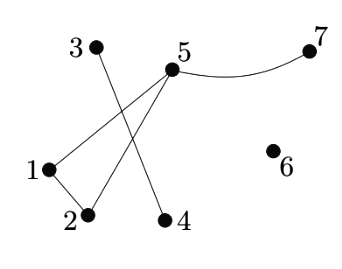
\includegraphics[scale=0.5]{Imagen1.png}
    \end{center}
    \caption{\footnotesize Example of a simple, undirected graph. In this case, $V=\lbrace 1,2,3,4,5,6,7 \rbrace$ and $E=\lbrace \lbrace 1,2 \rbrace , \lbrace 1,5 \rbrace , \lbrace 2,5 \rbrace , \lbrace 3,4 \rbrace , \lbrace 5,7 \rbrace \rbrace$.}
    \label{fig1}
\end{figure}

The number of vertices of a graph $G$ is its order, written as $|G|$; its number of edges is denoted by $\Vert G \Vert$. Graphs are finite, infinite, countable and so on according to their order.
An edge $e$ is called incident with a vertix $a$ if $e$ contains $a$, i.e. $e=\lbrace a,b\rbrace$ with $b \in V$. When the vertices $a,b \in V$ are the endpoints of an edge, they are referred to as being adjacent.

\textit{Definition 2.1} \textbf{Paths and cycles} A $\lbrace a,b \rbrace$-path is an ordered list of vertices $a=a_1,a_2,\ldots,a_{n-1},a_{n=b}$, such that for all $i$, vertices $a_i$ and $a_i+1$ are adjacent. A cycle is a path wherein a vertex is reachable from itself. The number of vertices of a path is the lenght of the path.

\textit{Definition 2.2} \textbf{Connected graph} A connected graph is a graph that has a $ \lbrace a,b \rbrace$-path for any two vertices $a,b \in V$. Otherwise we say it is a disconnected graph.

\textit{Definition 2.3} \textbf{Complete graph} A complete graph is a graph such that all vertices of $G$ are pairwise adjacent, i.e. every pair of vertices is connected by an edge. For a given number of vertices, there is a unique complete graph which is written as $K_N$, where $N$ is the number of vertices.

Note that every complete graph is necessarily connected, but connected graphs are not necessarily complete.

\begin{figure}[H]
    \begin{center}
        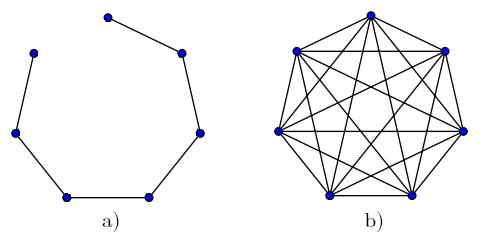
\includegraphics[scale=0.6]{completegraph.png}
    \end{center}
    \caption{\footnotesize Two types of connected graphs for the case of seven vertices: (a) The linear graph and (b) the complete graph, i.e. fully connected.}
    \label{complete}
\end{figure}


\textit{Definition 2.4} \textbf{Adjacency matrix} The adjacency relation gives rise to an adjacency matrix $\Gamma_G$ associated with a graph. If $V=\lbrace a_1, \ldots , a_N \rbrace$, then the adjacency matrix $\Gamma_G$ is a symmetric matrix $N\times N$, with elements,
\begin{equation}
\left( \Gamma_G\right)_{ij}=\left\lbrace \begin{array}{cc} 1 &  \lbrace a_{i},a_{j}\rbrace \in E \\ 0 & \textup{otherwise} \end{array}\right.
\end{equation}
\textbf{Remark} For weighted graphs 
\begin{equation}
\left( \Gamma_G\right)_{ij}=\lbrace \begin{array}{cc} \varphi_{a_{i}a_{j}} & , \lbrace a_{i},a_{j}\rbrace \in E \\ 0 & , \textup{otherwise} \end{array} 
\end{equation}
where $\varphi_{a_{i}a_{j}} \in \Re $.

\textit{Definition 2.5} \textbf{Neighborhood} The neighborhood of vertix $a$, written as $N_a$, is the set of vertices $b$ connected with $a$ with an edge. 
\begin{equation}
N_{a}= \lbrace b \in V | \lbrace a,b \rbrace \in E \rbrace
\end{equation}
In other words, the neighborhood is the set of vertices adjacent to a given vertex. The degree of vertix $a$ is the size of its neighborhood, $d(a)= |N_a|$. A vertex $a\in V$ with an empty neighborhood will be called isolated vertex.
In the study of graphs, we are mostly interested in problems that are invariant under permutations of the vertices when these permutations respect the neighborhood relation, i.e., map neighbored vertices onto neighbored vertices. Such permutations are called graph isomorphisms.

\textit{Definition 2.6} \textbf{Isomorphic graphs}  Let consider two graphs $ G= (V,E)$, $G'=(V',E')$ and $|V|=|V'|$. We say $G$ and $G'$ are isomorphic, $G\simeq G'$ if there exist a bijection $\phi : V\rightarrow V'$ such that
\begin{equation}
\lbrace a,b \rbrace \in E \Longleftrightarrow \lbrace \phi(a),\phi(b)\rbrace \in E'
\end{equation}
for all $a,b \in V$. The map $\phi$ is called an isomorphism. We usually do not distinguish between isomorphic graphs. Note that the number of isomorphic graphs grows exponentially with the number $N$ of vertices.

We set $G\cup G' := (V \cup V', E \cup E')$ and $G\cap G' := (V \cap V', E \cap E')$.
If $G\cap G'= \varnothing$ then $G$ and $G'$ are disjoint. If $V'\subseteq V$ and $E'\subseteq E$ then $G'$ is a subgraph of $G$, $G'\subseteq G$ (and $G$ a supergraph of $G'$). Less formally, we say that $G$ contains $G'$.

Consider a graph $G=(V,E)$, we can execute some manipulations and obtain new graphs from it. We will talk about the graph obtained from $G$ by deleting vertix $a \in V$ and all edges incident with $a$, written$G \backslash a$; the graph obtained from $G$ by deleting all $a \in A\subseteq V$ and all edges incident with $a$, $G \backslash A$ and the graph obtained from $G$ by deleting all edges $e \in F\subseteq E$, $G \backslash F$. 

Besides deleting vertices and edges, we can also join elements of graph $G$ to other sets. For a set of edges $F \subseteq [V]^2$, we will write the graph obtained from $G$ by cupping all edges $e \in F$, $G \cup F:= (V, E \cup F)$ and the graph obtained from $G$ by adding all edges $e \in F$, $ G + F:= (V,E + F)$, where
\begin{equation}
E + F = (E \cup F )\setminus(E \cap F )
\end{equation}
is the symmetric difference of $E$ and $F$.

\textit{Definition 2.7} \textbf{Complement graph} The complement $\overline{G}$ of graph $G$ is the graph on $V$ with edge set
\begin{equation}
\overline{E}=\lbrace (a,b)\in [V]^{2}:(a,b)\not\in E \wedge a\neq b\rbrace
\end{equation}

\begin{figure}[H]
    \begin{center}
        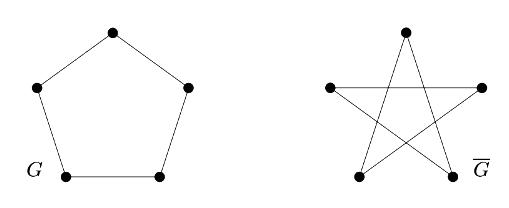
\includegraphics[scale=0.5]{Imagen2.png}
    \end{center}
    \caption{\footnotesize Example of a graph and its complement. In this particular case, $G$ is isomorphic to $\overline{G}$.}
    \label{fig2}
\end{figure}

\subsection{Tree graphs} 
A tree is an undirected graph in which any two vertices are connected by exactly one path. Every graph that does not contain any cycle is a tree, and viceversa. A forest is a disjoint union of trees. Thus, a forest is a graph whose components are trees. The vertices of degree $1$ in a tree are called leaves.
\begin{figure}[H]
    \begin{center}
        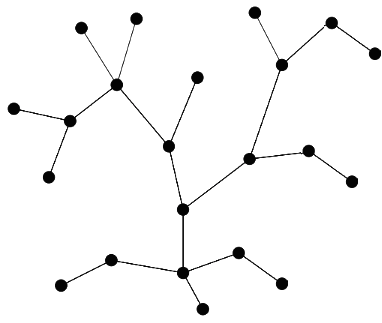
\includegraphics[scale=0.5]{Tree.png}
    \end{center}
    \caption{\footnotesize A tree }
    \label{figtree}
\end{figure}
\begin{prop}
Consider a graph $T$, the following assertions are equivalent:
\begin{enumerate}[(i)]
\item $T$ is a tree;
\item Any two vertices of $T$ are linked by a unique path in $T$;
\item $T$ is minimally connected, i.e. $T$ is connected but $T\setminus e$ is disconnected for every edge $e \in T$;
\item $T$ is maximally acyclic, i.e. $T$ contains no cycle but $T + \lbrace a,b\rbrace$ does, for any two non-adjacent vertices $a,b \in T$.
\end{enumerate}
\end{prop} 
We will write $\lbrace a,T,b \rbrace$ for the unique path in a tree $T$ between two vertices $a,b \in T$. Every connected graph $G$ admits a spanning tree, which is a tree that contains every vertex of $G$ and whose edges are edges of $G$. For any three vertices in a tree, the three paths between them have exactly one vertex in common.

Sometimes it is convenient to consider one vertex of a tree as special; such a vertex $r\in V$ is then called the root of this tree. A tree $T$ with a fixed root is a rooted tree. The edges of a rooted tree can be assigned a natural orientation, either away from or towards the root, in which case the structure becomes a directed rooted tree.
When a directed rooted tree has an orientation away from the root, it is called an arborescence, branching, or out-tree; when it has an orientation towards the root, it is called an anti-arborescence or in-tree. The tree-order is the partial ordering on the vertices of a tree, with $a<_{T}b$ for $a \in \lbrace r,T,b\rbrace$ if and only if the unique path from the root $r$ to $b$ passes through $a$. We say that $a$ lies below $b$ in $T$.

\begin{theorem}
A connected graph with $N$ vertices is a tree if and only if it has $N-1$ edge.\end{theorem} 
\begin{proof} Induction on $(i)$ shows that the subgraph spanned by the first
$i$ vertices has $i-1$ edges; for $i=N$ this proves the forward implication. Conversely, let $G$ be any connected graph with $N$ vertices and $N-1$ edges. Let $G'$ be a spanning tree in $G$. Since $G'$ has $N-1$ edges by the first implication, it follows that $G=G'$.
\end{proof}

\subsection{Colouring}
A vertex colouring of a graph $G=(V,E)$ is a map $c: V \rightarrow S$ such that $c(v)\neq c(w)$ for any adjacent vertices $v,w \in V$. The elements of the set $S$ are called the available colours. We shall be asking for the smallest integer k such that
$G$ has a $k$-colouring, a vertex colouring $c: V\rightarrow \lbrace 1,\ldots , k\rbrace$. This k is the vertex-chromatic number of $G$ and it is denoted by $\chi (G)$. A graph $G$ with $\chi (G)=k$ is called $k$-chromatic; if $\chi (G)\leq k$, the graph $G$ is called $k$-colourable.

For $k=2$, $2$-colouring of a graph is a map $c:V \rightarrow \lbrace 1,2 \rbrace$ such that all adjacent vertices are associated with a different element from $\lbrace 1,2 \rbrace$, which can be identified with two colors. Note that a $k$-colouring is nothing but a vertex partition into $k$ independent sets, now called colour classes. The non-trivial 2-colourable graphs are precisely the bipartite graphs.
\begin{figure}[H]
    \begin{center}
        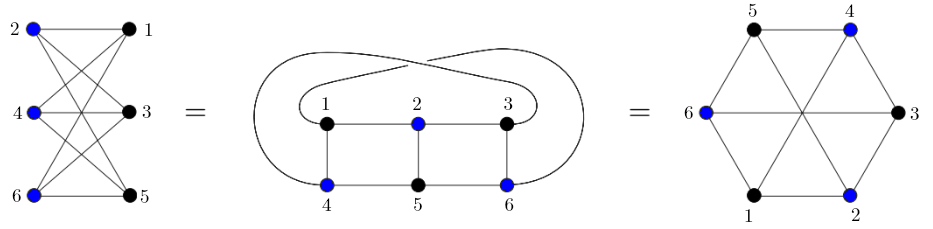
\includegraphics[scale=0.5]{Imagen4.png}
    \end{center}
    \caption{\footnotesize Three different representations of the same bipartite graph.}
    \label{fig4}
\end{figure}

An edge colouring of $G = (V,E)$ is a map $c: E\rightarrow S$ such that $c(e)\neq c(f)$ for any adjacent edges $e,f \in E$. The smallest integer $k$ for which a $k$-edge-colouring exists, i.e. an edge colouring $c: E\rightarrow \lbrace 1,\ldots , k\rbrace$, is the edge-chromatic number of $G$ and it is denoted by $\chi^{'}(G)$.

\subsection{Partitions}
In the multi-partite case we can group vertices into different partitions and study different features as multipacks, entanglement between partitions, etc. A partition of $V$ will be any tuple $(A_{1},\ldots ,A_{N})$ where $A_{i}\subset V$ are disjoint sets with $\bigcup^{N}_{i=1} A_{i}=V$. We will write 
\begin{equation}
\left( A_{1},\ldots ,A_{N}\right) \leqslant \left( B_{1},\ldots ,B_{N'}\right)
\end{equation}
if $\left( A_{1},\ldots ,A_{N}\right)$ is finier than $\left( B_{1},\ldots ,B_{N'}\right)$ meaning that for every $A_i$ then is $B_j$ with $A_{i}\subset B_{j}$. We say that $B_j$ is a coarser partition.

\section{Bipartite graphs}
Let $r\geq 2$ be an integer. A graph $G=(V,E)$ is called $r$-partite if the set of vertices $V$ admits a partition into $r$ classes such that every edge has its ends in different classes, i.e. vertices in the same partition class must not be adjacent. An $r$-partite graph in which every two vertices from different partition classes are adjacent is called complete and it is denoted by $K_{n_{1},\ldots ,n_{r}}$ where $n_i$ is the number of vertices in partition $i$. If $n_{1}=\ldots =n_{r}:=s$, we simply write $K^{r}_{s}$. Thus, $K^{r}_{s}$ is the complete $r$-partite graph in which every partition class contains exactly $s$ vertices.

A bipartite graph is a $2$-partite graph, i.e. its set of vertices can be partitioned into two disjoint sets, often called sinks or sources, such that no two vertices within the same set are adjacent.
\begin{figure}[H]
    \begin{center}
        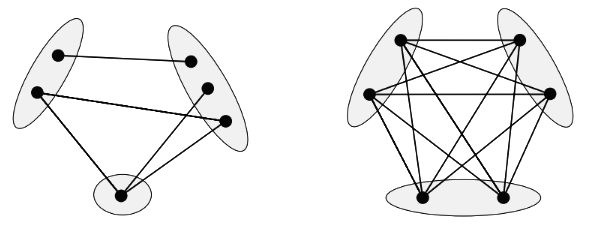
\includegraphics[scale=0.5]{Imagen3.png}
    \end{center}
    \caption{\footnotesize Example of two $3$-partite graphs.}
    \label{fig3}
\end{figure}

\begin{theorem}
A graph is bipartite if and only if it contains no cycle of ood lenght.
\end{theorem}
\begin{proof}
Consider a graph $G=(V,E)$ without odd cycles. A graph is bipartite if all its components are bipartite or trivial, so we may assume that $G$ is connected. Since every connected graph admits a spanning tree, let $T$ be a spanning tree in $G$, let $r\in T$ be its root, and denote the associated tree-order on $V$ by $\leqslant_T$. For each $v\in V$, the unique path $\lbrace r,T,v\rbrace$ has odd or even length. This defines a bipartition of $V$; thus we show that $G$ is bipartite with this partition.
\begin{figure}[H]
    \begin{center}
        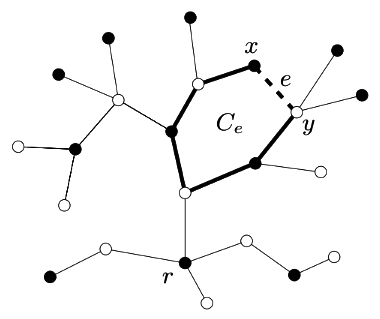
\includegraphics[scale=0.5]{Imagen5.png}
    \end{center}
    \caption{\footnotesize The cycle $C_e$ in graph $T+e$.}
    \label{fig5}
\end{figure}
Now let $e=\lbrace a,b \rbrace$ be an edge of a complete graph $G$. If $e\in T$, with $a<_{T}b$, then the unique path $\lbrace r,T,b \rbrace = \lbrace r,T,a,b\rbrace$ and so $a$ and $b$ lie in different partition classes and $G$ is bipartite. If $e\not\in T$ then $C_e:= \lbrace a,T,b\rbrace + e$ is a cycle, and by the case treated already the vertices along $\lbrace a,T,b\rbrace$ alternate between the two classes and $a$ and $b$ again lie in different classes, and $C_e$ is an even cycle.
\end{proof}

\begin{corollary}
Every tree is a bipartite graph.
\end{corollary}

\textit{Definition 2.8} \textbf{Star graph} A complete bipartite graph of the form $K_{1, N-1}$, i.e. a single vertex belongs to one set and all the remaining vertices belong to the other set, is called star graph and it is denoted by $S_{N,a}$ or $ST_{N,a}$ where $a \in V$ is the lone vertex. 

Consider a bipartition $(A,B)$ of the graph $G=(V,E)$. The subgraph $G_{AB}=(V,E_{AB})$ is induced by the edges $E_{AB}\equiv E(A,B)$ between $A$ and $B$ and $\Gamma_{AB}$ will denote the $|A|\times |B|$-off-diagonal submatrix of adjacency matrix $\Gamma_G$:
\begin{equation}
\Gamma_G = \left(\begin{array}{cc} \Gamma_{A} & \Gamma^{T}_{AB} \\ \Gamma_{AB}& \Gamma_{B} \end{array}\right)
\end{equation}
and similarly 
\begin{equation}
\Gamma_{G_{AB}} = \left(\begin{array}{cc} 0 & \Gamma^{T}_{AB} \\ \Gamma_{AB}& 0 \end{array}\right)
\end{equation}

\section{Equivalent graphs}\label{sec:eqGRAPH}
\subsection{Local Complementation}
Local complementation is a fundamental operation on graphs.
\begin{prop}[Local Complementation] Local complementation $\tau_v$ (LC) is a graph operation specified by a vertex $v\in V$, transforming a graph $G=(V,E)$ into $\tau_{v}(G)$ by replacing the induced subgraph on the neighborhood of $v$, i.e. $G[N_v]$, by its complement.
The neighborhood of any vertex $u$ in the new graph $\tau_{v}(G)$ is therefore given by
\begin{align}
N^{\tau_{v}(G)}_{u} &= \left\lbrace \begin{array}{cc} N_{u}\Delta (N_{v}\setminus \lbrace u \rbrace) & if \, (u,v)\in E \\ N_u & else \end{array}
\end{align}
where $\Delta$ is the symmetric difference between two sets. Given a sequence of vertices $\textbf{v} =\lbrace v_{1},\ldots , v_{k}\rbrace$ , we denote the induced sequence of local complementations, acting on a graph $G$, as
\begin{equation}
\tau_{\textbf{v}}(G)=\tau_{v_k}\circ \cdots \circ \tau_{v_1}(G)
\end{equation}
\label{LComplementation} 
\end{prop}
If two graphs $G_1$ and $G_2$ are related by a sequence of local complementations, i.e. $\exists \textbf{v} : \tau_{\textbf{v}}(G_1)=G_2$, we say the two graphs LC-equivalent and we write $G_{1}\sim_{LC} G_2$. Starting with a graph, the complete orbit can be obtained by succesively applying local complementation to the vertices in the preceding graph.

\textbf{Remark} Consider a vertex set $V$. For a vertex $c\in V$ of the star graph $S_{|V|,c}$ we have that $\tau_{c}(S_{|V|,c})=K_{|V|}$ and for any $v\in V$ we have $\tau_{v}(K_{|V|})=S_{|V|,v}$. This means all star graphs on a vertex set $V$ are equivalent to each other under local complementation and also to the complete graph on $V$ . Moreover, no other graph is equivalent to the star or complete graph.

\begin{figure}[H]
    \begin{center}
        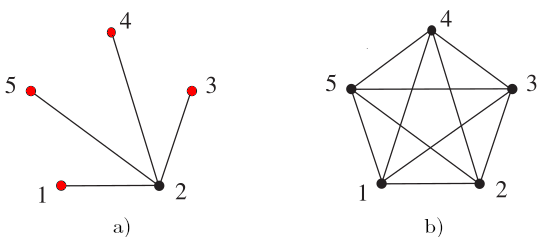
\includegraphics[scale=0.6]{LC.png}
    \end{center}
    \caption{\footnotesize The star graph (a) and the complete graph (b) are related by a single local complementation operation. Red vertices represent the neighborhood of vertex $2$.}
    \label{figLC}
\end{figure}
\subsection{Vertex-deletion}
Another fundamental operation on a graph is that of vertex-deletion, which we will see it relates to measuring a qubit of a graph state in the standard basis. 
\begin{lemma}[Vertex-deletion] Consider the graph $G=(V,E)$ and vertices $u,v \in V$ such that $u\neq v$, then
\begin{equation}
\tau_{v}(G\setminus u)=\tau_{v}(G)\setminus u
\end{equation}
This implies that on a graph $G=(V,E)$ local complementation and vertex-deletion are exchangeable.
\label{vertex}
\end{lemma}
\begin{proof} We need to prove that graphs $G_1 =\tau_{v}(G \setminus u)$ and $G_2 =\tau_{v}(G)\setminus u$ are equal, and to do this we show that the neighborhoods of all vertex in the graphs are the same, i.e. $N^{G_1}_w = N^{G_2}_w $ for all $w \in V \setminus u$. We have seen that local complementation $\tau_{v}(G)$ only changes the neighborhoods for vertices which are adjacent to $v$, so for any vertex $w \neq u$ which is not adjacent to $v$, we have that
\begin{equation}
N^{G_1}_w =N^{G_2}_w =N^{G}_w \setminus \lbrace u \rbrace
\end{equation}

If vertex $w$ is adjacent to $v$ its neighborhood becomes
\begin{equation}
N^{G_1}_w = (N^{G}_w \setminus \lbrace u \rbrace )\Delta \left(( (N^{G}_v \setminus \lbrace u \rbrace ) \setminus \lbrace w \rbrace \right)= \left(( (N^{G}_w \Delta (N^{G}_v \setminus \lbrace w \rbrace ) \setminus \lbrace w \rbrace \right) \setminus \lbrace u \rbrace =N^{G_2}_w 
\end{equation}
by the definition of a local complementation.
\end{proof}


\textit{Definition 2.9} \textbf{Vertex-minor} A graph $G'$ is called a vertex-minor of $G$, i.e. $G' < G$ if and only if there exist a sequence of local complementations and vertex-deletions that takes $G$ to $G'$. Since vertex-deletions can always be performed last in a sequence of local complementations (see \autoref{vertex}), an equivalent definition is the following: 
\begin{equation}
G' < G \\ \Longleftrightarrow \\ \tau_{\textbf{v}}(G)[V(G')]=G
\end{equation}
where $\textbf{v}$ is a sequence of local complementations.

\begin{corollary}
If two graphs $G_{1},G_{2}$ are LC-equivalent, then $G' < G_1$ if and only if $G' < G_2$.
\end{corollary}

\section{Quantum system}
We can associate with each vertix $a\in V$ a two-level quantum system with Hilbertspace $\mathcal{H}^a\cong \mathbb{C}^2$ or qubit. The state vector of the single–qubit system $\mathcal{H}^a$ can be written as
\begin{equation}
\ket{\psi}^{a}=\alpha \ket{0}^{a}+\beta \ket{1}^{a}
\end{equation} 
with $|\alpha|^2 + |\beta|^2 =1$. Consider the Pauli matrices of this two–level system
$\sigma^{a}_i = \lbrace \mathbb{I}^a , \sigma^{a}_x , \sigma^{a}_y , \sigma^{a}_z \rbrace$ with $i=0,1,2,3$, where the upper index specifies the Hilbert space on which the operator acts.
\begin{equation}
\sigma^{a}_i=\left\lbrace \left( \begin{array}{cc}1&0\\0&1 \end{array}\right),\left(\begin{array}{cc}0&1\\1&0 \end{array}\right),\left(\begin{array}{cc}0&-i\\i&0 \end{array}\right),\left(\begin{array}{cc}1&0\\0&-1 \end{array}\right) \right\rbrace
\end{equation}

Note that these operators form an orthogonal basis of Hermitian operators with respect to the scalar product $\braket{A,B}:= tr(A^{\dagger}B)$. The vectors $\ket{0}\equiv \ket{+,z}$ and $\ket{1}\equiv \ket{-,z}$ are the eigenvectors of the Pauli matrix $\sigma_z$ with eigenvalues $+1$ and $-1$. Alternatively, we could use the vectors $\ket{+}=\frac{1}{\sqrt{2}}(\ket{0}+\ket{1})\equiv \ket{+,x}$ and $\ket{-}=\frac{1}{\sqrt{2}}(\ket{0}-\ket{1})\equiv \ket{-,x}$, which are the eigenvectors of the Pauli matrix $\sigma_x$ with eigenvalues $+1$ and $-1$.
\begin{align}
\sigma_{z} \ket{\pm,z}&=\pm \ket{\pm,z}\\
\sigma_{x} \ket{\pm,x}&=\pm \ket{\pm,x}
\end{align}

In general $\overrightarrow{n}\cdot\overrightarrow{\sigma}\ket{\pm , \overrightarrow{n}}=\pm \ket{\pm , \overrightarrow{n}}$, where $\overrightarrow{n}=(n_x ,n_y ,n_z)$ and $\overrightarrow{\sigma}=(\sigma_x , \sigma_y , \sigma_z)$.

The Pauli group $\mathcal{P}:=\braket{\lbrace \pm 1, \pm i \rbrace\times \lbrace \sigma^{a}_0 , \sigma^{a}_1 , \sigma^{a}_2 ,\sigma^{a}_3 \rbrace}$, is the set of all Pauli matrices up to phase factor $\pm 1, \pm i $. We will frequently use the projectors onto the eigenvectors of the Pauli operators. For example,
\begin{equation}
P^{a}_{z,\pm}=\frac{1 \pm \sigma^{a}_z}{2}=\ket{\pm ,z}^a \bra{\pm ,z}
\end{equation}
denotes the projector onto the eigenvector $\ket{\pm ,z}$ of $\sigma^{a}_z$ with eigenvalue $\pm 1$, and similarly for $\sigma^{a}_x$ and $\sigma^{a}_y$.

Consider the subset of vertices $A \subset V$, with aim to simplify notations we use sets and subsets as an upper index for states and operators. They denote the respective tensor product of a given state or sets, e.g. $\ket{+}^{V}=\bigotimes_{v \in V} \ket{+}^{v}$. Other examples are
\begin{center}
\begin{matrix}
$\mathcal{H}^V =\bigotimes_{v \in V} \mathcal{H}^{v}$& $\sigma^{A}_{z} =\bigotimes_{a \in A} \sigma^{a}_z$\\
$\mathcal{P}^V=\bigotimes_{v \in V} \mathcal{P}^{v}$&$\mathcal{P}^{A}_{x,+}=\bigotimes_{a \in A} \mathcal{P}^{a}_{x,+}\equiv  \ket{+}^A\bra{+}$\\
\end{matrix}
\end{center}

\subsection{Binary notation}
We identify the subset $A \subset V$ with its corresponding binary vector, $A=(A_i)_{i \in V}\simeq(A_{1}, A_{2},\ldots ,A_N)$ over the binary field $\mathbb{F}^{V}_2$ (add multiples modulo $2$).

\underline{Example:} Consider the graph $G=(V,E)$, with set of vertices $V=\lbrace 1,2,3,4, \rbrace$. We can use set and binary notation in the same formula $A=\lbrace 1,4 \rbrace\simeq (1,0,0,1)$.

These notations allow us to use set and binary operations in the same formula. For example, for $A,B \in \mathcal{P}(V)\simeq \mathbb{F}^{V}_2$ we will simply write $A \cup B$, $A \cap B$ and $A \setminus B$ for the union, intersection and difference (complement) as well as $A+B$ and $\braket{A,B}$ for the addition and the scalar product modulo 2.



\chapter{Graph States}\label{chap:Graphs states}
\section{Introduction}
A key concept in realizing quantum technologies is the preparation of specific resource states, which then will be used for quantum processing purposes. An important class of such resource states are graph states. These states can be described by a simple undirected and unweighted graph where the vertices correspond to the qubits of the state. Graph states can be regarded as the result of an interaction of particles initially prepared in some product state, however not all interaction patterns can be represented reasonably by a simple graph.

An important feature of graph states is that they can be efficiently described classically. To describe a graph state of $n$ qubits, only $\frac{n(n−1)}{2}$ bits are needed in contrast to the $2^n$ complex numbers required to describe a general quantum state. It turns out that for graph states, their evolution under Clifford operations and Pauli measurement can be simulated efficiently on a classical computer \cite{NielsenChuang},\cite{Vidal}.

Graph states form a family of multiqubit states which includes many popular states such as the Greenberger-Horne-Zeilinger (GHZ) state and the cluster states.

\begin{figure}[H]
    \begin{center}
        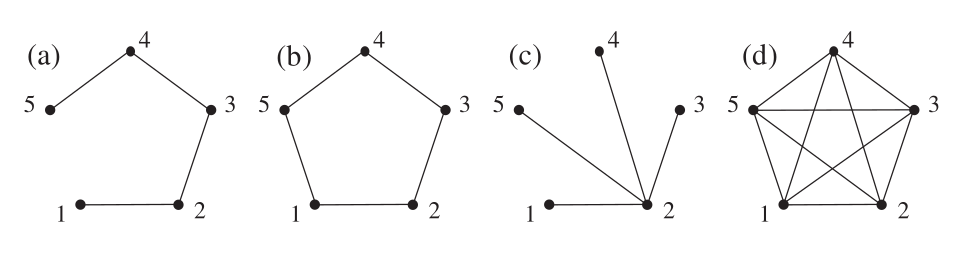
\includegraphics[scale=0.4]{ImagenPentagono.png}
    \end{center}
    \caption{\footnotesize Types of graphs for the case of five vertices: (a) The linear cluster graph, (b) the ring cluster graph, (c) the star graph $S_5$, which describes a GHZ state, and (d) the
complete graph $K_5$. Note that this graph can be obtained from $S_5$ by local complementation on the second qubit, so it also describes a GHZ state.}
    \label{figPentagono}
\end{figure}

Graph states are useful for many applications: in characterization of computational resources in measurement based quantum computing models, in entanglement measurement and purification, in quantum error-correcting codes all codes correspond to graph states, the one-way quantum computation uses graph states as resources.

In the following sections we will see the concept of graph state from two perspectives. First, we will introduce the description of graph states in terms of the interaction pattern and show that such a definition is also meaningful if all particles interact with the same Ising-type interaction. Then, we will see a description in terms of the class of states that correspond to a simple graph and how these states can be described efficiently in terms of their stabilizer, which is a subgroup of the Pauli group. We will explain local unitary equivalence between graph states and discuss the relation to stabilizer states and illustrate an alternative representation of the stabilizer formalism in terms of its binary representation.

\section{Interaction pattern}

Consider a graph $G=(V,E)$ such that asociated with each vertex there is a two-level quantum system or qubit. The qubits are prepared in some initial state vector $\ket{\psi}$ and then they are coupled according to some interaction pattern. For each edge $\lbrace a,b \rbrace \in E$ the qubits of the two adjacent vertices $a$ and $b$ interact according to some (non-local) unitary $U_{ab} = e^{-i \varphi_{ab} H_{ab}}$, where $H_{ab}$ is the interaction Hamiltonian and $\varphi_{ab}$ is the coupling strength\footnote{$\varphi_{ab}$ can also be understood as the interaction time $\varphi_{ab}=\int^{t}_{0}d\tau g_{ab}(\tau)$ in the unitary time-evolution $U_{ab}\left(\varphi_{ab}\right)=e^{-\frac{i}{\hbar}\int^{t}_{0}d\tau H_{ab}(\tau)}$}. The most general of such interaction pattern has to be represented by the graph $G$.
Under which conditions can this be completely specified by a simple graph $G$?
For characterizing a large class of interaction patterns, the two–particle unitaries should fulfill the following: 
\begin{enumerate}[(i)]
\item Since the graph $G$ does not provide any ordering of the edges unitaries $U_{ab}$ must commute:
\begin{equation}
\left[ U_{ab},U_{b,c} \right]=0 \quad \forall a,b,c \in V 
\end{equation}
\item Since we are considering undirected graphs, unitaries $U_{ab}$ must be symmetric:
\begin{equation}
U_{ab}=U_{ba} \quad \forall a,b \in V
\end{equation}
\item Since we are considering unweighted graphs, all unitaries $U_{ab}$ are the same for all qubits:
\begin{equation}
U_{ab}=U^{\lbrace a,b \rbrace} \quad \forall a,b \in V
\end{equation}
\end{enumerate}

\begin{prop}[Ising interactions] Any interaction pattern in which the qubits interact according to some two–particle unitaries chosen from a set of commuting interactions can alternatively be described by a pure Ising interaction according to the same graph and some local z-rotations\footnote{$V^{\alpha}=e^{i\beta_a \sigma^{a}_{z}}$} to be applied before or after the coupling operation.
\begin{equation}
U^{I}_{ab}(\varphi_{ab}):=e^{-i\varphi_{ab}\sigma^{a}_{z}\sigma^{b}_{z}}
\end{equation}
where the interaction Hamiltonian is $H^{I}_{ab}=\sigma^{a}_{z}\sigma^{b}_{z}$ and $\sigma^{a}_{x},\sigma^{a}_{y},\sigma^{a}_{z}$ are the Pauli matrices acting on qubit $a$..
\end{prop}

\begin{proof} Consider two different unitaries $U=e^{iH}$ and $\tilde{U}=e^{i\tilde{H}}$, where $H$ and $\tilde{H}$ are hermitian operators and two setting of three vertices $a,b,c \in V$. We have that:
\begin{equation*}
U_{ab}=U^{\lbrace a,b \rbrace}=\tilde{U}^{\lbrace a,b \rbrace} \:  \textrm{and} \: U_{bc}=U^{\lbrace b,c \rbrace}=\tilde{U}^{\lbrace b,c \rbrace}
\end{equation*}
\begin{equation*}
\left[ H^{\lbrace a,b \rbrace}, \tilde{H}^{\lbrace b,c \rbrace}\right]=0 \:  \textrm{and} \: \left[ \tilde{H}^{\lbrace a,b \rbrace}, H^{\lbrace b,c \rbrace}\right]=0
\end{equation*}
We have used the fact that $\left[ f(A),f(B)\right]=0$ if and only if $[A,B]=0$. Every hermitian operator allows for a real decomposition with respect to the basis of Pauli operators $\lbrace \sigma_{0}, \sigma_{x}, \sigma_{y}, \sigma_{z} \rbrace$, i.e., $H^{a,b} = \sum_{ij}A_{ij}\sigma^{a}_{i}\sigma^{b}_{j}$. By local unitaries we can diagonalize one of the Hamiltonians, $H^{a,b} = \sum_{i}A_{i}\sigma^{a}_{i}\sigma^{b}_{i}$ and represent the other one with respect to this basis, i.e., $\tilde{H}^{b,c} = \sum_{jk}B_{jk}\sigma^{b}_{j}\sigma^{c}_{k}$. Therefore we have
\begin{equation}
\sum_{ijk}A_{i}B_{jk}\sigma^{a}_{i}\otimes [\sigma_i ,\sigma_j]^{b} \otimes \sigma^{c}_k =0
\end{equation}
from which it follows:
\begin{equation}
\forall i,j =1,2,3 \: \textrm{with} \: i\neq j \: : \quad A_i = 0 \vee B_{jk}=0 \: \forall k = 0,1,2,3
\end{equation}
If $H$ corresponds to a non-trivial two-body interaction up to a (local) change of basis we can assume that $A_3 \neq 0$. If another component, e.g. $A_2 \neq 0$, then all components in $B$ except $B_{00}$ vanish, and therefore $\tilde{H}$ is a trivial interaction. If instead $A_1 = A_2 = 0$, then at least all components in $B$ apart from $B_{00} , B_{03} , B_{30}$ and $B_{33}$ have to vanish. Any terms due to $B_{03}$ or $B_{30}$ correspond to local z-rotations and all these rotations commute with the Ising interaction terms $H^{I}_{ab}=\sigma^{a}_{z}\sigma^{b}_{z}$. 

We have shown that this Ising interaction $H^{I}_{ab}=\sigma^{a}_{z}\sigma^{b}_{z}$ fulfills conditions $(i)$ and $(ii)$ since it is symmetric. Condition $(iii)$ implies that we have to fix the interaction strenght $\varphi_{ab}$. For simple graphs we will choose $\varphi = \frac{\pi}{4}$.
\end{proof}

The unitary two-qubit operator $U_{ab}$ is generated by an Ising-type interaction. Consider the interaction Hamiltonian:
\begin{align}
\nonumber H_{ab}&=\frac{\mathbb{I}-\sigma^{a}_{z}}{2}\otimes \frac{\mathbb{I}-\sigma^{b}_{z}}{2}=\ket{1}^{a}\bra{1}\otimes \ket{1}^{b}\bra{1} \\ &=  P^{a}_{z,-}\otimes P^{b}_{z,-}= \frac{1}{4}\left( \mathbb{I}- \sigma^{a}_{z}-\sigma^{b}_{z} + H^{I}_{ab} \right)
\end{align}
It generates the unitary transformation known as controlled phase gate:
\begin{align}
U_{ab}\left(\varphi_{ab}\right)&=e^{-i\varphi_{ab}H_{ab}}
\end{align}
We find 
\begin{align}
U_{ab}(\varphi_{ab})&=e^{-i \frac{ \varphi_{ab}}{4}}e^{i \frac{\varphi_{ab}}{4} \sigma^{a}_{z}}e^{i\frac{\varphi_{ab}}{4} \sigma^{b}_{z}}e^{-i\frac{\varphi_{ab}}{4}\sigma^{a}_{z}\sigma^{b}_{z}} \\
&=e^{-i\frac{\varphi_{ab}}{4} }e^{i\frac{\varphi_{ab}}{4} \sigma^{a}_{z}}e^{i\frac{\varphi_{ab}}{4} \sigma^{b}_{z}}U^{I}_{ab}\left(\frac{\varphi_{ab}}{4}\right)
\end{align}

Note that the phase gate corresponds to the Ising intercation up to some additional $\frac{\pi}{4}$-rotations around $z$-axes at each qubit, and the corresponding interaction strength now is $\varphi_{ab}=\pi$. Thus the control phase gate is generated by Ising interaction with phase $\varphi_{ab}=\pi$.
\begin{equation}
U_{ab}(\pi)= P^{a}_{z,+}\otimes \mathbb{I}^{b} + P^{a}_{z,-}\otimes \sigma^{b}_{z}= \ket{0}^{a}\bra{0}\otimes \mathbb{I}^{b} + \ket{1}^{a}\bra{1}\otimes \sigma^{b}_{z}
\end{equation}

\begin{proof}
\begin{align*}
 e^{-i\pi P^{a}_{z,-}\otimes P^{b}_{z,-}&= \sum^{\infty}_{k=0} \frac{(-i\pi)^{k}}{k!}\left(P^{a}_{z,-}\otimes P^{b}_{z,-}\right)^{k} \\ 
&= \mathbb{I}+ \left( \sum^{\infty}_{k=1} \frac{(-i\pi)^{k}}{k!}\right)^{k}\left(P^{a}_{z,-}\otimes P^{b}_{z,-}\right)^{k} \\ 
&=  \mathbb{I}+ \left( e^{-i\pi}-1\right)^{k}\left(P^{a}_{z,-}\otimes P^{b}_{z,-}\right)^{k} \\ 
&=  \mathbb{I}^{a}\otimes \mathbb{I}^{b} -2\left(P^{a}_{z,-}\otimes P^{b}_{z,-}\right) \\
& =  \left(P^{a}_{z,+} + P^{a}_{z,-}}\right)\otimes \left(P^{b}_{z,+} + P^{b}_{z,-}\right) - 2 \left(P^{a}_{z,-}\otimes P^{b}_{z,-}\right)\\ 
&=  \left(P^{a}_{z,+}\otimes P^{b}_{z,+}\right) + \left(P^{a}_{z,+}\otimes P^{b}_{z,-}\right) + \left(P^{a}_{z,-}\otimes P^{b}_{z,+}\right) - \left(P^{a}_{z,-}\otimes P^{b}_{z,-}\right) \\
&=  P^{a}_{z,+}\left(P^{b}_{z,+}+ P^{b}_{z,-}\right)+P^{a}_{z,-}\left(P^{b}_{z,+}- P^{b}_{z,-}\right) \\
&=  P^{a}_{z,+} \otimes \mathbb{I}^{b} + P^{a}_{z,-}\otimes \sigma^{b}_{z}=U_{ab}
\end{align*}
\end{proof}

This gate corresponds to a controlled $\sigma_z$ on qubits $a,b$, i.e.
\begin{equation}
U_{ab}=\ket{0}\bra{0}\otimes \mathbb{I}^b + \ket{1}^{a}\bra{1}\otimes \sigma^{b}_z= \left( \begin{array}{cccc}
 1 & 0 & 0 & 0\\
0 & 1 & 0 & 0\\
0 & 0 & 1 & 0\\
0 & 0 & 0 &-1\\ 
\end{array} \right)
\end{equation}

\textbf{Remark} The phase gate $U_{ab}$ creates and deletes the edge $\lbrace a,b \rbrace$ in a graph $G$ depending on whether the edge is already existing.

Consider the state vector over all vertices $v\in V$:
\begin{equation}
\ket{\psi}=\ket{+}^{V}=\ket{+}^{v_1}\otimes \ket{+}^{v_2} \cdots \otimes \ket{+}^{v_n}
\end{equation}
If we apply control phase gate $U_{ab}$ on two qubits at vertices $a,b$ with state $\ket{+}$ this ensures that the resulting state vector
\begin{equation}
U_{ab}\ket{+}^{a}\ket{+}^{b}=\frac{1}{\sqrt{2}}\left( \ket{0}^{a}\ket{+}^{b} + \ket{1}^{a}\ket{-}^{b}\right)
\end{equation}
is maximally entangled, i.e. is a Bell state. 

\begin{prop}[Graph States I]
Let $G=(V,E)$ be a simple graph. The graph state $\ket{G}$ associated with $G$ can be written as the pure state:
\begin{equation}
\ket{G}=\prod_{\lbrace a,b \rbrace \in E} U_{ab} \ket{+}^{V}
\end{equation}
Where $U_{ab}$ is the control phase gate and $\ket{+}^{V}$ is the initial state. Note that $\ket{+}^{V}$ can be regarded as the graph state corresponding to the empty graph.
\end{prop}
The preparation procedure is as follows:
\begin{enumerate}
\item Qubits at each vertex are prepared in the pure state with state vector $\ket{+}$
\item Phase gate $U_{ab}$ is applied to every pair of vertices $a,b$ such that $\lbrace a,b \rbrace \in E$.
\end{enumerate}

\begin{figure}[H]
    \begin{center}
        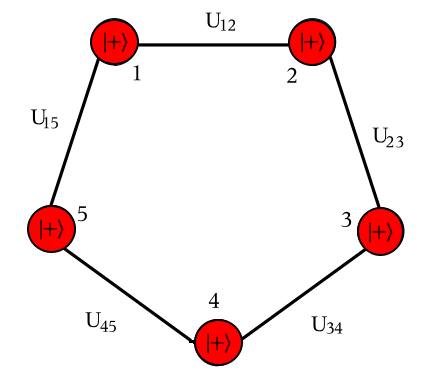
\includegraphics[scale=0.5]{graphstate1.png}
    \end{center}
    \caption{\footnotesize Preparation procedure to obtain a graph state that corresponds to a ring graph.}
    \label{gs1}
\end{figure}


\section{Stabilizer formalism}\label{sec:Stabilizer}
Apart from the interaction pattern, graph states can also be defined uniquely in terms of their stabilizer.

\textit{Definition 3.1} \textbf{Stabilizer subgroup} Consider a group $H$ acting on a set $X$. For all $x \in X$ the stabilizer subgroup of $H$ with respect to $x$ is defined as the set of elements in $H$ that leave $x$ fixed:
\begin{equation}
\mathcal{S}_x=\lbrace h\in H | h \cdot x =x \rbrace
\end{equation}

Consider two elements $ x, y \in X$, and consider the group element $h$ such that $y = h⋅x$. Then the two stabilizer groups $\mathcal{S}_x$ and $\mathcal{S}_Y$ are related by $\mathcal{S}_y = h \cdot \mathcal{S}_x \cdot h^{-1}$, i.e. the stabilizers of elements in the same orbit are conjugate to each other.

\begin{proof} By definition, $z \in \mathcal{S}_y$  if and only if $z\cdot(h\cdot x) = h\cdot x$. Applying $h^{-1}$ to both sides of this equality yields $(h^{-1}zh)\cdot x = x$; that is, $h^{-1}\cdot z\cdot h \in \mathcal{S}_x$. An opposite inclusion follows similarly by taking $z \in \mathcal{S}_x$ and supposing $x = h^{-1}\cdot y$.
\end{proof}  

A subgroup of Pauli matrices $\mathcal{S}\subset \mathcal{P}^V$ is a stabilizer on $n$ qubits if and only if $\mathcal{S}$ is an abelian group which does not include $-\sigma^{\otimes n}_0$. The elements $M_i(i = 1, \ldots ,l)$ are called generators of $\mathcal{S}$ if every element $M\in \mathcal{S}$ can be written as a product $M=M^{x_1}_1 M^{x_2}_2 \cdots M^{x_l}_l$ with $x_i \in \lbrace 0,1\rbrace$. If $l=n$, the elements in $\mathcal{S}$ will have only one common eigenvector with eigenvalue 1. We call this unique common eigenvector as stabilizer state. 

Then, a stabilizer state $\ket{S}$ is the unique normalized state satisfying $M\ket{S}=\ket{S}$ for every $M \in \mathcal{S}$. It is easy to see that the density matrix of a stabilizer state $\ket{S}$ is
\begin{equation}
\rho_{\mathcal{S}}=\ket{S}\bra{S}=\frac{1}{2^n}\sum_{M \in \mathcal{S}} M
\label{eq:stabilizer}
\end{equation} 


\begin{prop}[Graph States II]
Let $G=(V,E)$ be a simple graph. The graph state $\ket{G}\in \mathcal{H}^V$ corresponding to $G$ is the unique common eigenstate of a set of $N=|V|$ commuting observables
\begin{equation}
K_{a}=\sigma^{a}_{x}\sigma^{N_a}_{z}=\sigma^{a}_{x}\prod_{b\in N_a}\sigma^{b}_{z} \quad a=1,2,\ldots N
\end{equation}
where $\sigma^{a}_{x},\sigma^{a}_{y},\sigma^{a}_{z}$ are the Pauli matrices acting on qubit $a$ and $N_a$ is the neighborhood of qubit $a$.
\end{prop}

\begin{figure}[H]
    \begin{center}
        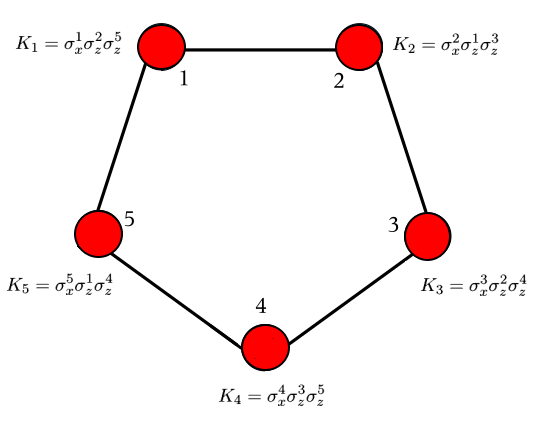
\includegraphics[scale=0.5]{graphstate2.png}
    \end{center}
    \caption{\footnotesize The stabilizing operator $K_a$ for a ring graph state of 5 vertices.}
    \label{gs2}
\end{figure}

The eigenvalues of the stabilizing operators $K_a$ are $+1 \ \forall a \in V$, that is the graph state $\ket{G}$ associated with the graph $G$ fulfills
\begin{equation}
K_{a}\ket{G}=\ket{G}, \forall a \in V 
\end{equation}
  
The stabilizer group of a graph state $\ket{G}$ is the abelian subgroup $\mathcal{S}$ of Pauli group $\mathcal{P}^V$ that is generated by the set $\lbrace K_{a} | a \in V \rbrace$.  

\begin{proof}
Consider the initial state $\ket{+}^V$, with no correlations. The eigenvalues of $\ket{+}^V$ are $\sigma^{a}_{x}\ket{+}^V=\ket{+}^V , \forall a \in V$. We consider the vertix $a \in V$, choose $b \in N_{a}$ and compute theconjugation of $\sigma^{a}_{x}$ with $U_{ab}$.
\begin{align}
U_{ab} \sigma^{a}_{x} U^{\dagger}_{ab} &= \left( \ket{0}^{a}\bra{0}\otimes \mathbb{I}^{b} + \ket{1}^{a}\bra{1}\otimes \sigma^{b}_{z} \right) \sigma^{a}_{x} \left(\ket{0}^{a}\bra{0}\otimes \mathbb{I}^{b} + \ket{1}^{a}\bra{1}\otimes \sigma^{b}_{z}\right) \\ 
&= \sigma^{a}_{x} \left(\ket{1}^{a}\bra{1}\otimes \mathbb{I}^{b} + \ket{0}^{a}\bra{0}\otimes \sigma^{b}_{z}\right)\left(\ket{1}^{a}\bra{1}\otimes \mathbb{I}^{b} + \ket{0}^{a}\bra{0}\otimes \sigma^{b}_{z}\right) \\
& = \sigma^{a}_{x} \left( 0 + \ket{0}^{a}\bra{0}\otimes \sigma^{b}_{z} + \ket{1}^{a}\bra{1}\otimes \sigma^{b}_{z} + 0 \right) \\
& = \sigma^{a}_{x}\sigma^{b}_{z}
\end{align}
If we iterate with all neighbors of $a$ we get:
\begin{equation}
\left(\prod_{b \in N_a} U_{ab}\right)\sigma^{a}_{x}\left(\prod_{b \in N_a} U^{\dagger}_{ab}\right)= \sigma^{a}_{x} \prod_{b \in N_a} \sigma^{b}_{z} \\
= \sigma^{a}_{x}\sigma^{N_a}_{z} = K_a
\end{equation}
Now consider the eigenvalues equation $\sigma^{a}_{x}\ket{+}^V=\ket{+}^V , \forall a \in V$.
\begin{equation}
\left(\prod_{\lbrace a,b \rbrace \in E} U_{ab}\right)\sigma^{a}_{x}\left(\prod_{\lbrace a,b \rbrace \in E} U^{\dagger}_{ab}\right)\left(\prod_{\lbrace a,b \rbrace \in E} U_{ab}\right)\ket{+}^{V}= \left(\prod_{\lbrace a,b \rbrace \in E} U_{ab}\right)\ket{+}^V
\end{equation}

Since $\left(\prod_{\lbrace a,b \rbrace \in E} U_{ab}\right)\sigma^{a}_{x}\left(\prod_{\lbrace a,b \rbrace \in E} U^{\dagger}_{ab}\right)=K_a$. If the edges are not in the neighborhood they are in different Hilbert spaces, other $U_{cb}$ with $c\neq a$ can be pulled through $\sigma^{a}_{x}$.
\begin{equation}
K_{a}\left(\prod_{\lbrace a,b \rbrace \in E} U_{ab}\right)\ket{+}^V=\left(\prod_{\lbrace a,b \rbrace \in E} U_{ab}\right)\ket{+}^V , \forall a \in V
\end{equation}
\begin{equation}
\left(\prod_{\lbrace a,b \rbrace \in E} U_{ab}\right)\ket{+}^V=\ket{G}  
\end{equation}
\end{proof}  
  
The stabilizing operator $K_a=\sigma^{a}_{x}\sigma^{N_a}_{z}$ gives rise to a measurement pattern of the vertices of the graph, the qubit at vertex $a$ is measured in $x$-direction and the vertices $b$ in $N_b$ in $z$-direction.
Physically, the generators $K_a$ describe the perfect correlations in the state $\ket{G}$, since $\braket{G|K_a|G}=\braket{\sigma^{a}_{x}\prod_{b\in N_a}\sigma^{b}_{z}}=1$. Then $K_a$ provides constraints to the correlations between the measurement outcomes $m^{a}_{x} = \pm 1$ and $m^{b}_{z} = \pm 1$, namely
\begin{equation}
m^{a}_{x} \prod_{b \in N_a}m^{b}_{z}=1
\end{equation}

\subsection{Graph state basis}
For each $\ket{G}$ associated with the graph $G$ we have $2^{N-1}$ states with similar properties in $\mathcal{H}^{V}$. Consider the subset of vertices $W \subset V$ defined by:
\begin{equation}
\ket{W}=\sigma^{W}_{z}\ket{G}\equiv \prod_{\sigma^{a}_{z}}\ket{G}
\end{equation}
The states $\ket{W}$ are eigenstates of the correlation operator $K_a$ with different eigenvalues $W_a$ and satisfy:
\begin{equation}
K_{a}\ket{W}=(-1)^{\delta_{W}(a)}\ket{W}\equiv (-1)^{W_a}\ket{W}
\end{equation}
where $\delta_{W}(a)=\left\lbrace \begin{array}{cc} 1 & a \in W \\ 0 & otherwise \end{array}\right\rbrace=W_a$ and that introduces the binary vector $w=(w_{1},w_{2}\ldots w_{N})$ associated with set $W$.

\begin{proof}
$$K_{a}\ket{W}=K_{a}\prod_{b\in W} \sigma^{b}_{z}\ket{G}=(-1)^{\delta_{w}(a)}\prod_{b\in W} \sigma^{b}_{z}K_{a}\ket{G}$$
We know that $K_{a}\ket{G}=\ket{G}$ and $\prod_{b\in W}\ket{G}=\ket{W}$. Then,
\begin{equation}
K_{a}\ket{W}= (-1)^{\delta_{w}(a)} \ket{W} \ \forall a \in V 
\end{equation}
\end{proof}

The set $\lbrace \ket{W}=\sigma^{W}_{z}\ket{G} | w\subseteq V\rbrace$ forms a basis of $\mathcal{H}^{V}=(\mathbb{C}^2)^V$ with completeness relation $\sum_{W \subset V}\ket{W}\bra{W}=\mathbb{I}^{V}$.

For two different subsets $W,W' \subseteq V$ the states $\ket{W}$, $\ket{W'}$ have list of eigenvalues $(w_1,\ldots , w_N)$ and $(w'_1,\ldots , w'_N)$ which differ in at least one item, that is $\exists \; a \in V | w_{a}\neq w'_{a}$. This implies $\braket{w|w'}=\delta_{ww'}$, with $\lbrace K_{a}| a\in V\rbrace$ is a set of commuting observables. There are $2^N$ differents subsets $W \subseteq V$, therefore there exist $2^N$ pair-wise orthogonal eigenstates $\ket{W}$ and $\lbrace \ket{W}|W \subseteq V\rbrace$ form a basis of $\mathcal{H}^V$.

The proyector onto a graph state has a direct representation in terms of the corresponding stabilizer $\mathcal{S}$ :
\begin{equation}
\ket{G}\bra{G}=\frac{1}{2^N}\sum_{\sigma \in \mathcal{S}} \sigma
\label{eq:proyector}
\end{equation}
where
\begin{equation}
\lbrace K^{s_1}_{1},K^{s_2}_{2} \ldots K^{s_N}_{N} | (s_{1},\ldots, s_{N}) \in \lbrace 0,1\rbrace^{N} \rbrace = \mathcal{S}
\end{equation}
\begin{proof}
First, we consider the right-hand side of \autoref{eq:proyector}.
\begin{equation}
\braket{W|rhs|W'}=\frac{1}{2^N}\sum_{\sigma \in S} \braket{W|\sigma |W'}= \frac{1}{2^N}\sum^{1}_{s_{1},\ldots, s_{N}=0} \braket{W|K^{s_1}_{1},K^{s_2}_{2} \ldots K^{s_N}_{N} |W'}
\end{equation}

We know that $\bra{W}=\bra{G}\sigma^{W}_{z}$ and $\ket{W'}=\sigma^{W'}_{z}\ket{G}$. Besides, pulling the $Ks$ through gets a sign $\pm 1$. 
\begin{align}
\braket{G|\sigma^{W}_{z}K^{s_1}_{1},K^{s_2}_{2} \ldots K^{s_N}_{N}\sigma^{W'}_{z}|G}&= (-1)^{\delta_{w}(1)s_1}\ldots (-1)^{\delta_{w}(N)s_N}\braket{G|\sigma^{W}_{z}\sigma^{W'}_{z}|G} \\
&= \nonumber (-1)^{\delta_{w}(1)s_1}\ldots (-1)^{\delta_{w}(N)s_N} \braket{W|W'} \\
&= (-1)^{\sum_{a \in W}s_a}\delta_{WW'}
\end{align}
Therefore, for $|V|=N$ and $|W|=M \ M \leq N$, 
\begin{equation}
\braket{W \ket{G}\bra{G} W'}= \frac{1}{2^N}\sum^{1}_{s_{M+1}, \ldots, s_{N}=0}\left( \sum^{1}_{s_{1}, \ldots, s_{M}} (-1)^{\sum_{a \in W}s_a}\right) \delta_{WW'}
\end{equation}

For $W\neq \emptyset$ there are $2^{|W|}-1$ asignements for $\lbrace s_{a} | a \in W\rbrace$ with $\sum_{a \in W}s_a= \textup{even}$ and same number with $\sum_{a \in W}s_a= \textup{odd}$. Then, 
\begin{align}
\sum^{1}_{s_{1}, \ldots, s_{M}} (-1)^{\sum_{a \in W}s_a} &= \left\lbrace \begin{array}{cc} 0 & W \neq\emptyset \\ 2^{M} & W=\emptyset \end{array}
\end{align}


\begin{equation}
\frac{1}{2^N} 2^{N-M} 2^{M}\delta_{WW'}\delta_{W\emptyset}= \delta_{WW'}\delta_{W\emptyset} \ \forall W,W'
\end{equation} 

Now we consider the left-hand side of \autoref{eq:proyector}.
\begin{equation}
\braket{W|lhs|W'}=\braket{W|G}\braket{G|W'} = \delta_{W\emptyset} \delta_{W' \emptyset} \ \forall W,W' 
\end{equation}
\end{proof}
\subsection{Binary representation}
We now briefly review an alternative representation of the stabilizer formalism in terms of its binary representation, which allows one to treat the properties of the stabilizer in terms of a symplectic subspace of the vector space $\mathbb{F}^{2N}_2$. A more detailed description of binary representation can be found in \cite{EinGS},\cite{GraphDescLC}. 

Every element of the Pauli group $U \in \mathcal{P}^{V}$ can be written uniquely, up to a phase factor, in form:
\begin{equation}
U=\sigma^{\textbf{U}_x}_{x} \sigma^{\textbf{U}_z}_{z}= \prod_{a \in V} \sigma^{U^{a}_x}_{x}\prod_{a \in V} \sigma^{U^{a}_z}_{z}
\end{equation}
with $U^{a}_{x},U^{a}_{z} \in \lbrace 0,1 \rbrace$ for every $a\in V$

Therefore, we can introduce a mapping denoted by $\mathcal{B}$ which maps the elements of $\mathcal{P}^V$ to a $2N$-dimensional binary vectors as follows:
\begin{equation}
\mathcal{B}: U=\sigma^{U_x}_{x} \sigma^{U_z}_{z} \rightarrow (U_{x}|U_{z}) \in \mathbb{F}^{2N}_{2} 
\end{equation}
For single qubits this is
\begin{center}
\begin{matrix}
$\sigma_{0} \rightarrow (0|0)$&$\sigma_{x} \rightarrow (1|0)$\\
$\sigma_{y} \rightarrow (1|1)$&$\sigma_{z} \rightarrow (0|1)$\\
\end{matrix}
\end{center}
and for example the correlation operator $K_1$ in \autoref{gs2} has the binary representation
$$K_1=\sigma^{1}_{x}\sigma^{2}_{z}\sigma^{5}_{z} \rightarrow (10000|01001)$$

The binary representation has the following two important properties: letting $u,w,x \in \mathcal{P}^V$ with corresponding binary vectors $\textbf{U}, \textbf{V}, \textbf{X} \in \mathbb{F}^{2N}_{2}$, one finds that:
\begin{enumerate}[(i)]
\item $u \ w \sim x \quad \longleftrightarrow \quad \textbf{U}+\textbf{W}=\textbf{X}$ (mod 2)
\item $[u,w]=0 \quad \longleftrightarrow \quad \textbf{U}^{T}\textbf{P}\textbf{W}=0$ (mod 2)
\end{enumerate}
where $\sim$ denotes equality up to a global phase factor and matrix \textbf{P} written
$$\textbf{P}=\left( \begin{array}{c|c} 0 & 1 \\ \hline 1 & 0 \\ \end{array} \right)$$
defines the symplectic inner profuct on the binary space $\mathbb{F}^{2N}_{2}$. From property (i) it follows that the mappin $\mathcal{B}$ is a homomorphism of groups and property (ii) shows that two Pauli operators commute if and only if the corresponding binary vectors are orthogonal with respect to the symplectic inner product.

Consider the stabilizer state $\ket{S}$,i.e. $M \ket{S}=\ket{S}$, $\forall M \in \mathcal{S}$. The correlation operators can be written in binary representaion as follows:
\begin{align}
 S_{1}&=\sigma^{x_1}_{x} \sigma^{z_1}_{z} \rightarrow (x_{1}|z_{1}) \in \mathbb{F}^{2N}_{2} \\
 \nonumber \vdots \\
S_{N}&=\sigma^{x_N}_{x} \sigma^{z_N}_{z} \rightarrow (x_{N}|z_{N}) \in \mathbb{F}^{2N}_{2} 
\end{align}

We can summarize this in terms of a generator matrix $(\textbf{X}|\textbf{Z})$ where \textbf{X} and \textbf{Z} are $N \times N$ matrices, which is a full rank $2N \times N$. A generator matrix is obtained by assembling all binary representations of a set of independent stabilizer generators as the rows of the matrix.

$$\textbf{X}=\left( \begin{array}{c} x_1 \\ \vdots \\ x_N \end{array}\right) \ \ \textbf{Z}=\left( \begin{array}{c} z_1 \\ \vdots \\ z_N \end{array}\right)$$

The generator matrix for graph state $\ket{G}$ has a normal form:
\begin{equation}
(\textbf{X}|\textbf{Z})=\left( \mathbb{I} \mid \Gamma \right)
\end{equation}
where $\Gamma$ is the adjacent matrix of graph $G$.

\underline{Example:} GHZ state for three particles $\ket{\phi}_{123}=\frac{1}{\sqrt{2}}\left(\ket{000}+\ket{111}\right)$.
$$S_{1}=x_{1}x_{2}x_{3} \rightarrow (111|000)$$
$$S_{2}=z_{1}z_{2} \rightarrow (000|110)$$
$$S_{3}=z_{2}z_{3} \rightarrow (000|011)$$
So the generator matriz for GHZ state is
$$(\textbf{X}|\textbf{Z})=\left( \begin{array}{ccc|ccc} 1&1&1& 0&0&0\\
0&0&0&1&1&0 \\
0&0&0&0&1&1
\end{array}\right)$$

\section{Equivalent graph states}

Through definitions, each graph $G$ uniquely specifies a graph state $\ket{G}$ and viceversa. In other words, two different graphs $G=(V,E)$ and $G'=(V,E')$ cannot describe the same graph state.

\begin{proof}
Suppose $\exists G=(V,E) , G'=(V,E')$ with $E\neq E'$and $\ket{G}=\ket{G'}$.
\begin{equation}
 \ket{G}=\ket{G'} \rightarrow \prod_{\lbrace a,b \rbrace \in E}U_{ab}\ket{+}^{V}= \prod_{\lbrace a,b \rbrace \in E'}U_{ab}\ket{+}^{V}
\end{equation}
\begin{equation}
U_{ab}=U^{-1}_{ab} \rightarrow \ket{+}^{V}= \prod_{\lbrace a,b \rbrace \in E+E'}U_{ab}
\end{equation}
Then $E+E'= \emptyset \rightarrow E=E' \rightarrow \textup{Contradicction}$
\end{proof}

On the other hand, two differents graphs $G=(V,E) , G'=(V,E')$ can describe two graph states $\ket{G}\neq\ket{G'}$ that are identical up to same local unitary transformations $U=U_{1},U_{2},\ldots ,U_{N} \in U^{N}(2)$. We say two graphs $G=(V,E) , G'=(V,E')$ are LU-equivalent and we write $\ket{G'}\simeq_{LU}\ket{G}$ if there exists a local unitary $U \in \textbf{U}(2)^{V}$ such that
\begin{equation}
\ket{G'}=U\ket{G}
\end{equation}

Suppose that $\mathcal{S}$ is the stabilizer subgroup of $\ket{G}$, i.e. $s\ket{G}=\ket{G} \forall s \in \mathcal{S}$ and $\ket{G'}=U\ket{G}$. Then denoting,
\begin{equation}
\sum'=U\mathcal{S}U^{\dagger}=\lbrace UsU^{\dagger} | s \in \mathcal{S} \rbrace
\end{equation}
we find that $s'\ket{G'}=\ket{G'}$ for all $s' \in \sum'$. In this sense the group $\sum '$ is a stabilizing subgroup of the state vector $\ket{G'}$, however in general (for general $U$) $s'$ is not the tensor product of Pauli group, that is $\sum'$ is not a subgroup of Pauli group $\mathcal{P}^V$. But for certain $U$, $\sum' \in \mathcal{P}^V$. 

\subsection{Local Clifford operations}
We now look for local unitaries $U \in \textbf{U}^{V}(2)$, for which $U\mathcal{P}^{V}U^{\dagger}=\mathcal{P}^{V}$, meaning that $U$ maps the whole Pauli group $\mathcal{P}^{V}$ onto itself under conjugation. The set of unitaries
\begin{equation}
\mathcal{C}^{V}_{1}:=\lbrace U \in \textbf{U}^{V}(2) | U\mathcal{P}^{V}U^{\dagger}=\mathcal{P}^{V} \rbrace
\end{equation}
is a group and it is called local Clifford group of $N=|V|$ qubits. If $\ket{G}$ and $\ket{G'}$ are graph states and $\ket{G'}=U\ket{G}$ for $U \in \mathcal{C}^{V}_{1}$ then $\sum'=UsU^{\dagger}=s'$ is the stabilizer of $\ket{G'}$. 

Therefore, local Clifford operations on graph states can entirely be described within the stabilizer formalism – and this is one of the main reasons why the local Clifford group is of central importance in the context of graph states. We will say two graph states $\ket{G}$ and $\ket{G'}$ are LC-equivalent, and we write $\ket{G}\simeq_{LC}\ket{G'}$, if and only if $\exists \; U \in \mathcal{C}^{V}_{1}$ such that $\ket{G'}=U\ket{G}$.
 
The Local Clifford group $\mathcal{C}^{V}_{1}:=\mathcal{C}^{\otimes V}_{1}$ on N qubits is the N-fold tensor product of $\mathcal{C}_{1}$ with itself. The one-qubit Clifford group $\mathcal{C}_1$ is the normalizer of $\mathcal{P}_1$ in $\textbf{U}(2)$, i.e. it is the subgroup of $2\times 2$ unitary operators which map $\mathcal{P}_1$ to itself under conjugation. It is defined by
\begin{equation}
\mathcal{C}_{1}=\lbrace U \in U(2)|UPU^{\dagger}=P\rbrace=\braket{H,S}
\end{equation}
where the set of $2\times 2$ unitary operators $\lbrace H,S \rbrace$ is the generator of the group, up to a global phase factor.
\begin{enumerate}[(i)]
\item $H$ corresponds to Hadamard gate and generates rotations around $45^{\circ}$ axis in $xy, xz, yz$ plane with angle $\pi$.
\begin{equation}
H=\frac{1}{\sqrt{2}}\left( \sigma_{x}+\sigma_{z}\right)=\frac{1}{\sqrt{2}}\left(\begin{array}{cc}1&1\\1&-1 \end{array}\right) 
\end{equation}
\item $S$ corresponds to single-qubit phase gate and generates rotations around $x,y,z$ with angle $\frac{\pi}{2}$.
\begin{equation}
S=\sqrt{\sigma_{z}}=\left(\begin{array}{cc}1&0\\0&i\end{array}\right) 
\end{equation}
\end{enumerate}

We can see intuitively the action of the two single-qubit gates $H$ and $S$ looking at the Bloch sphere in \autoref{Bloch}, where it is represented the pure state of a two-level quantum system $\rho=\frac{1}{2}(\mathbb{I}+\vec{s}\hat{\vec{\sigma}})$.
\begin{figure}[H]
    \begin{center}
        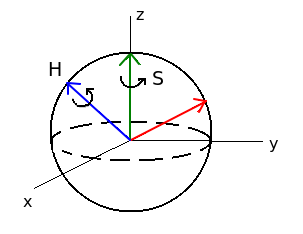
\includegraphics[scale=0.6]{BlochSphere.png}
    \end{center}
    \caption{\footnotesize Bloch sphere and representation of $H$ and $S$ operators.}
    \label{Bloch}
\end{figure}
The action of the Clifford group $\mathcal{C}_1$ under conjugation permutes the Pauli matrices $\sigma_x ,\sigma_y , \sigma_z$ up to a phase factor $\pm 1$.

\underline{Examples:} $H\sigma_{z}H^{\dagger}=\sigma_{x}$ , $H\sigma_{x}H^{\dagger}=\sigma_{z}$ , $S\sigma_{x}S^{\dagger}=\sigma_{y}$ , $S\sigma_{y}S^{\dagger}=-\sigma_{x}$
\begin{proof}
First, note that matrices $\pm \sigma_0$ and $\pm i\sigma_0$ are left unchanged under conjugation. The set $\lbrace \pm \sigma_x ,\pm\sigma_y ,\pm \sigma_z\rbrace$ has to be mapped onto itself, since $U\sigma_i U^{\dagger}$ is herminitian if and only if $\sigma_i$ is hermitian. Because the conjugation is invertible, it permutes the matrices $\sigma_x ,\sigma_y , \sigma_z$ up to some sign $\pm$. 
\end{proof}

Up to overall phase factors, the one-qubit Clifford group $C_{1}$ has finite cardinality $|C_{1} \backslash \lbrace e^{i\varphi}|\varphi\in [0,2\pi]\rbrace |=24$. Ref. \cite{EinGS} presents all 24 single-qubit Clifford unitaries and their decomposition in terms of Pauli operators and $\frac{\pi}{2}$-rotations.
Consider the $\frac{\pi}{2}$-rotation, i.e. rotation $e^{-i\frac{\alpha}{2}\vec{n}\vec{\sigma}}$ with rotation angle $\alpha=\frac{\pi}{2}$ around $\vec{n}$ axis. 
\begin{equation}
\sqrt{\pm i \sigma_{h}}=e^{\pm i \frac{\pi}{4}\sigma_{h}} \ , h=1,2,3 
\end{equation}
These rotations lead to elementary permutations, i.e. permutations of only two indices:
$$ \lbrace 1,2,3 \rbrace \\ \xrightarrow{\sqrt{\pm i \sigma_{1}}} \\ \lbrace 1,3,2 \rbrace$$
$$ \lbrace 1,2,3 \rbrace \\ \xrightarrow{\sqrt{\pm i \sigma_{2}}} \\ \lbrace 3,2,1 \rbrace$$
$$ \lbrace 1,2,3 \rbrace \\ \xrightarrow{\sqrt{\pm i \sigma_{3}}} \\ \lbrace 2,1,3 \rbrace$$

Instead of $H$ and $S$ any two of these elementary permutations can be used
to generate the Clifford group $\mathcal{C}_1$ .
\begin{proof}
We execute the explicit computation. For $\sigma_{z}$ we have
\begin{equation}
\sqrt{\pm i \sigma_{z}}=e^{\pm i \frac{\pi}{4}\sigma_{z}}=\cos \frac{\pi}{4}\mathbb{I} \pm i \sin \frac{\pi}{4}\sigma_{z}=\frac{1}{\sqrt{2}}\left( \mathbb{I}\pm i \sigma_{z} \right)
\end{equation}

And similar for $\sigma_{x}$ and $\sigma_{y}$. Therefore, $\sqrt{\pm i \sigma_{i}}$ for $i=1,2,3$ is equivalent to the $\pm \frac{\pi}{2}$-rotation around $x,y,z$ axis. Now, we do the following calculations.
\begin{equation}
\sigma_{z}\sqrt{+\sigma_{y}}=\sigma_{z}\frac{1}{\sqrt{2}}\left( \mathbb{I}+ i \sigma_{y} \right)= \frac{1}{\sqrt{2}}\left( \sigma_{x} + \sigma_{z} \right) = H \equiv H_{xz}
\end{equation}
\begin{equation}
\sigma_{x}\sqrt{+\sigma_{z}}=\sigma_{x}\frac{1}{\sqrt{2}}\left( \mathbb{I}+ i \sigma_{z} \right)= \frac{1}{\sqrt{2}}\left( \sigma_{x} + \sigma_{y} \right)=H_{xy}
\end{equation}
\begin{equation}
 \sigma_{x}\sqrt{-\sigma_{y}}=\sigma_{x}\frac{1}{\sqrt{2}}\left( \mathbb{I}- i \sigma_{y} \right)= \frac{1}{\sqrt{2}}\left( \sigma_{x} + \sigma_{z} \right)= H_{xz}
\end{equation}
\begin{equation}
\sigma_{x}\sqrt{+\sigma_{y}}=\sigma_{x}\frac{1}{\sqrt{2}}\left( \mathbb{I}+ i \sigma_{y} \right)=\frac{1}{\sqrt{2}}\left( \sigma_{x} - \sigma_{z} \right)=\vec{H_{xz}}
\end{equation}
So, these give rise to the rotations arround $45^{\circ}$ axes. 
\end{proof}

In conclusion, these operations generate all permutations and for that reason we can consider only operators $H$ and $\sqrt{i \sigma_{z}}$ as generators of Clifford group.
\begin{align*}
\sqrt{ i \sigma_{z}}\sqrt{ i \sigma_{z}}&= i \sigma_{z} \\
 H\sigma_{z}H &= \sigma_{x} \\
 H\sqrt{ i \sigma_{z}}H &= \sqrt{ i \sigma_{x}} \\ 
 i\sigma_{x}\sigma_{z}&=\sigma_{y} \\
 \sigma_{z}H&= \sigma_{z}\frac{1}{\sqrt{2}}(\sigma_{x}+\sigma_{z}) =\frac{1}{\sqrt{2}}(\mathbb{I}+i\sigma_{y})= \sqrt{ i \sigma_{y}}
\end{align*}

For a graph with $N=|V|$ vertices, we have $24^N$ different Clifford unitaries that generate its Clifford orbit. To decide whether two graph states are LC equivalent seem to be exponencially difficult, but there is in fact a polynomical method to calculate them.

\textit{Definition 3.2} \textbf{Clifford group} The Clifford group (on $N$ qubits) is the group of all unitary operators that map the Pauli group to itself under conjugation.
\begin{equation}
\mathcal{C}_{N}:=\lbrace U \in \textbf{U}(2^N) | U\mathcal{P}^{V}U^{\dagger}=\mathcal{P}^{V} \rbrace
\end{equation}
By definition, Clifford operations map stabilizer states to stabilizer states. Any Clifford operation $U$ can be decomposed, up to a global phase factor, into a sequence of $\mathcal{O}(N^2)$ one- and two-qubit gates in the set of generators $\braket{H,S,CNOT}$, where H and S are defined as before and $CNOT$ is the controlled-NOT gate
$$CNOT^{ab}=\ket{0}^{a}\bra{0}\otimes \mathbb{I}^b + \ket{1}^{a}\bra{1} \otimes \sigma^{b}_x=\left(\begin{array}{cccc}1&0&0&0 \\ 0&1&0&0 \\ 0&0&0&1 \\ 0&0&1&0\\ \end{array}\right)$$
\subsection{LC-Rule}
As we have seen previuosly, local Clifford operations on graph states can entirely be described within the stabilizer formalism. Let us consider the following sequence of single-qubit Clifford operations:
\begin{equation}
U^{\tau}_{a}(G)=e^{-i\frac{\pi}{4}\sigma^{a}_{x}}\prod_{b\in N_a}e^{i\frac{\pi}{4}\sigma^{b}_{z}} \propto \sqrt{K_a}
\label{lcunitary}
\end{equation}

The action of local Clifford operations on graph states can be described in terms of a simple graph transformation rule, called local complementation, defined in  \ref{LComplementation} in page \pageref{LComplementation}.

\begin{prop}[LC-rule] By local complementation of a graph $\ket{G}$ at some vertex $a\in V$ one obtains a LC-equivalent graph state:
\begin{equation}
\ket{\tau_{a}(G)}=U^{\tau}_{a}(G)\ket{G}
\end{equation}
where $\tau_a$ is a local complementation on vertex $a$ and $U^{\tau}_{a}(G)$ is a local Clifford unitary defined in \autoref{lcunitary}. Therefore, operation $U^{\tau}_{a}(G)$ on graph state $\ket{G}$ can be seen as an operation $\tau_a$ on the graph $G$.

Two graph states $\ket{G}$,$\ket{G'}$ are LC-equivalent if and only if the corresponding graph are related by a sequence of local complementation. That is
\begin{equation}
G'=\tau_{a_N}\cdot \tau_{a_{N-1}} \cdots \tau_{a_1}(G) \: \textup{with} \: \ a_{1}\ldots a_{N} \in V
\end{equation}
\end{prop}

\begin{figure}[H]
    \begin{center}
        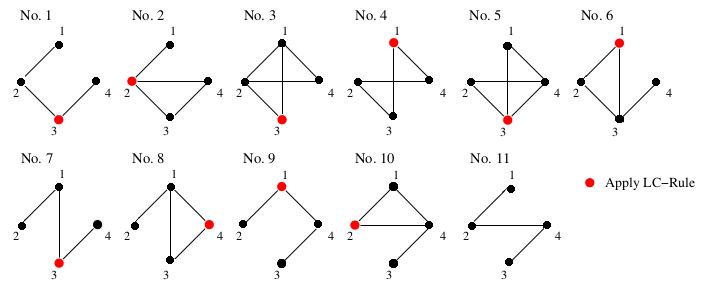
\includegraphics[scale=0.6]{lcrule.png}
    \end{center}
    \caption{\footnotesize Example for a succesive application of LC-rule, which exhibits the whole equivalence class associated with graph No.1.}
    \label{LCrule}
\end{figure}
\begin{proof}
Consider a graph $G$, with the corresponding graph state $\ket{G}$ and correlation operator $K_{b}\ket{G}=\ket{G} \ \ \forall b \in V$ and the graph obtained from local complementation at vertex $a$ $G':=\tau_{a}(G)$ with correlation operator $K_{b}'\ket{G'}=\ket{G'} \ \ \forall b \in V$. For  $c \in V \backslash N_{a}$, we have that
\begin{equation}
U^{\tau}_{a}K_{c}(U^{\tau}_{a})^{\dagger}= K_{c}=K^{'}_{c} 
\end{equation}
 
For $b \in N_{a}$ we find that
\begin{align}
U^{\tau}_{a}K_{b}(U^{\tau}_{a})^{\dagger}&= \left( \sqrt{ -i \sigma^{a}_{x}}\prod_{a' \in N_{a}} \sqrt{+i \sigma^{a'}_{z}} \right) \sigma^{b}_{x}\prod_{b'\in N_{b}} \sigma^{b'}_{z} \left( \sqrt{+i \sigma^{a}_{x}}\prod_{a' \in N_{a}} \sqrt{-i \sigma^{a'}_{z}} \right) \\ 
&= \sqrt{ -i \sigma^{a}_{x}} \sqrt{i \sigma_{z}^{N_a}} \sigma^{b}_{x}\sigma^{N_b}_{z}\sqrt{i \sigma_{x}^{a}}\sqrt{ -i \sigma_{z}^{N_a}}
\end{align}

We can  pull $\sqrt{i \sigma^{a}_{x}}$ in second place in the above equation and the only change could be just a phase $(\pm i)$, but we have to be careful because $a$ is in the neighborhood of $b$, so there is a $\sigma_{z}$ which not commute.
We can rewrite a few terms, $\sigma^{N_b}_{z}=\sigma^{N_{b}\backslash a}_{z}\sigma^{a}_{z}$ and $\sqrt{ -i \sigma^{N_a}_{z}}=\sqrt{ \sigma^{N_{a}\backslash b}_{z}}} \sqrt{-i \sigma^{b}_{z}}$. Then, pulling $\sqrt{i \sigma^{a}_{x}}$ in second place changes $i \rightarrow -i$, and pulling $\sqrt{-i \sigma^{b}_{z}}$  in second place changes $-i \rightarrow i$. This gives us the following:
\begin{equation}
(-i\sigma^{a}_{x})(i\sigma^{b}_{z})(\sigma^{b}_{x})(\sigma^{N_b}_{z})=\sigma^{a}_{x}\sigma^{b}_{z}\sigma^{b}_{x}\sigma^{N_b}_{z}
\end{equation}
We can rewrite the term $\sigma^{b}_z =\sigma^{N_a}_{z}\sigma^{N_{a}\backslash b}_{z}$.
\begin{align}
\sigma^{a}_{x}\sigma^{N_a}_{z}\sigma^{N_{a}\backslash b}_{z}\sigma^{b}_{x}\sigma^{N_b}_{z}&=\sigma^{a}_{x}\sigma^{N_a}_{z}\cdot \sigma^{b}_{x} (\sigma^{(N_{b}+N_{a}\backslash b)}_{z})\\
\sigma^{a}_{x}\sigma^{N_a}_{z}\cdot \sigma^{b}_{x} \sigma^{b'}_{z}&= K'_{a}\cdot K'_{b}
\end{align}

The stabilizer $U^{\tau}_{a}\mathcal{S}(U^{\tau}_{a})^{\dagger}$ of the state $U^{\tau}_{a}\ket{G}$ is thus generated by:
\begin{equation}
\lbrace K'_{c} \rbrace_{c \in V\backslash N_{a}} \cup \lbrace K'_{a} K'_{b} \rbrace_{b \in N_{a}} 
\end{equation}
By multiplying $K'_{a} K'_{b}$ with $K'_{a}$, one obtain a new generate set.
\begin{equation}
\lbrace K'_{c} \rbrace_{c \in V\backslash N_{a}} \cup \lbrace K'_{b} \rbrace_{b \in N_{a}} = \lbrace K'_{a} \rbrace_{a \in V}
\end{equation}
\begin{equation}
\Rightarrow K'_{a}\ket{G}=\ket{G'} \ \ \forall a \in V  
\end{equation}
This proves that by using the LC rule we obtain, standing from  a given state, a sequence of Local Clifford equivalents graph states.
\end{proof}

\begin{prop}[Stabilizer states] Any stabilizer state vector $\ket{S}$ is LC-equivalent to some graph state vector $\ket{G}$, i.e., $\ket{S}=U\ket{G}$ for some LC-unitary $U \in \mathcal{C}^V$. This unitary can be calculated efficiently.
\label{stabilizerstate}
\end{prop}
The proof of \autoref{stabilizerstate} can be found in \cite{GraphDescLC} in terms of binary description.

\section{Measurements on graph states}

\subsection{Local Pauli measurements}
The exact form of Local Pauli measurements can be found in \cite{MPEnGS} but  we will only focus on the results of the measurements over graph state $\ket{G}$.

\begin{prop}[Local Pauli measurements] A projective measurement of $\sigma_x , \sigma_y , \sigma_z$ on qubit associated with a vertex $a \in G$ yields, up to local unitaries $U^{a}_{i,\pm}$ a new graph state $\ket{G'}$ on the remaining vertices. The resulting graph $G'$ is
\begin{align}
P^{a}_{z,\pm}\ket{G}&=\frac{1}{\sqrt{2}}\ket{z,\pm}^{a}\otimes U^{a}_{z,\pm}\ket{G\setminus a}\\
P^{a}_{y,\pm}\ket{G}&=\frac{1}{\sqrt{2}}\ket{y,\pm}^{a}\otimes U^{a}_{y,\pm}\ket{\tau_{a}(G)\setminus a}\\
P^{a}_{x,\pm}\ket{G}&=\frac{1}{\sqrt{2}}\ket{x,\pm}^{a}\otimes U^{a}_{x,\pm}\ket{\tau_{b}\left(\tau_{a}\circ \tau_{b}(G)\setminus a\right)}
\end{align}
for $b \in N_a$. The local unitaries $U^{a}_{i,\pm}$ are given by:
\begin{center}
\begin{matrix}
$U^{a}_{z,+}=\mathbb{I}^{a}$&$U^{a}_{z,-}=\sigma^{N_a}_{z}$ \\
$U^{a}_{y,+}=\sqrt{-i\sigma^{N_a}_{z}}$&$U^{a}_{y,-}=\sqrt{+i\sigma^{N_a}_{z}}$\\
$U^{a}_{x,+}=\sqrt{+i\sigma^{b}_{y}}\sigma^{N_{a}\backslash (b \cup N_{b})}_{z}$&$U^{a}_{x,-}=\sqrt{-i\sigma^{b}_{y}}\sigma^{N_{b}\backslash (a \cup N_{a})}_{z}$
\end{matrix}
\end{center}
\end{prop}
For a sequence of local Pauli measurements, the local unitaries have to be taken into account if the graph state is unitarily transformed. A table with relevant commutation relations for Pauli projections and Clifford operations can be found in \cite{MPEnGS}. 

Consider a Pauli measurement $\sigma_x , \sigma_y , \sigm_z$ at a single vertex $a$ of a graph state $\ket{G}$. Notice that the resulting graph state $\ket{G'}$ can be obtained from the initial graph $G$: a $\sigma_z$-measurement is equivalent to deleting vertex $a$ from $G$, a $\sigma_y$-measurement is equivalent to replacing the subgraph $G[N_a]$ by its complement and deleting vertex $a$, and a $\sigma_x$-measurement is equivalent to replacing the subgraph $G[N_b]$, for any $b \in N_a$, by its complement, applying the rule for $\sigma_y$ and replacing $G[N_b]$ by its complement again.

\subsection{Clifford operations}
Clifford group are Clifford unitaries $U \in \mathcal{C}_N$ and Pauli measurements. Since it is possible to efficiently decompose an arbitrary Clifford unitary in terms of the one-qubit gates $H$, $S$ and two-qubit gate $CNOT$ (see definition 10), any Clifford operation can be simulated by a sequence of at most $\mathcal{O}(N^2)$ of these gates together with one Pauli measurement at a single vertex. Therefore, any Clifford operation can be efficiently simulated on a classical computer on polynomial time \cite{NielsenChuang}.

\begin{prop}[(Gottesman–Knill theorem] Any stabilizer circuit on a quantum register of $N$ qubits, which consists of $M$ steps, can be simulated on a classical computer using at most $\mathcal{O}(N^3 M)$ elementary classical operations.
\end{prop}

Indeed it has been shown that such classical simulator actually requires only $\mathcal{O}(N^2)$ elementary operations on classical computer. The Clifford group plays a crucial role in entanglement purification protocols and quantum error correcting codes, as many of them contain Clifford gates. 

\subsection{Connecting graph states}
Two graph states can be connected by appling two different methods, one where the two connection qubits are merged into one, and one where they are both projected out. Consider two graphs states $\ket{G},\ket{G'}$ with set of vertices $V,V'$ respectively. Let $a \in V$ and $b \in V'$ be two qubits corresponding to vertices of the two graph states.
\begin{itemize}
\item \textit{Connection 1}. We apply $CNOT$ operation between qubits $a,b$, $CNOT^{a\rightarrow b}=\ket{0}^{a}\bra{0}\otimes \mathbb{I}^b + \ket{1}^{a}\bra{1} \otimes \sigma^{b}_x$, followed by a $\sigma_z$-measurement on qubit $b$. The resulting state is a graph state (up to local Clifford unitaries) that corresponds to a graph without vertex $b$ (since we measured in $z$-basis) and the neighborhood of $a$ is given by $\tilde{N_a} = N_a \cup N_b -N_a \cap N_b$.
\item \textit{Connection 2}. We apply local complementation $\tau$ on both qubits $a,b$ obtaining graphs $\tau_a (G)$ and $\tau_b (G')$. Then we apply $CNOT^{a\rightarrow b}$ followed by a $\sigma_z$-measurement on qubit $b$ and $\sigma_y$-measurement on qubit $a$. he resulting state is a graph state (up to local Clifford unitaries) that corresponds to a graph without vertices $a$ and $b$ and edges according to $\tilde{N_i}=N_i\cup N_b -N_i \cap N_b$ for all $i \in N_a$ and $\tilde{N_j}=N_j \cup N_a -N_j \cap N_a$ for all $j \in N_b$.
\end{itemize}

\chapter{Quantum Entanglement}\label{chap:Entanglement}
Formally, we say a quantum state is entangled if it is not classically correlated, and classically correlated means that it can be prepared using physical devices locally, where all correlations are due to shared classical randomness. In contrast entangled states cannot be prepared using local physical devices alone. Correlations in classical systems can always be described in terms of classical probabilities; this is not always true in quantum systems, entanglement is a unique phenomenon of quantum mechanics.

Composite quantum systems are systems that naturally decompose into two or more subsystems, where each subsystem itself is a proper quantum system. The Hilbert space associated with a composite, or multipartite system, is given by the tensor product $\mathcal{H}=\mathcal{H}_1 \otimes \cdots \otimes \mathcal{H}_N$ of the spaces corresponding to each of the subsystems. In the following we shall focus on finite-dimensional bipartite quantum systems, i.e. systems composed of two distinct subsystems, described by the Hilbert space $\mathcal{H}=\mathcal{H}_A \otimes \mathcal{H}_B=\mathbb{C}^2 \otimes \mathbb{C}^2$. 

An entangled state of a bipartite system is a state that cannot be written as a product state of the component systems. Consider a two-qubit state
\begin{equation}
\ket{\psi^{+}}=\frac{1}{\sqrt{2}}(\ket{01}_{AB}+\ket{10}_{AB})
\end{equation}
This state cannot be written as a product state of $\ket{q}_A \ket{p}_B$ for $q,p \in \lbrace 0,1 \rbrace$. Quantum state $\ket{\psi^{+}}$ is maximally entangled, which means that when we trace over qubit $B$ to find the reduced density operator $\rho_A$ of qubit $A$ we obtain a multiple of identity operator
\begin{equation}
\rho_A = tr_B (\ket{\psi^{+}}\bra{\psi^{+}})=\frac{1}{2}\mathbb{I}_A
\end{equation}
(and similarly $\rho_B =\frac{1}{2}\mathbb{I}_B$). If we measure system $A$ in any basis the result will be completely random ($\ket{0}$ or $\ket{1}$ with equal probability $\frac{1}{2}$). Therefore, if we perform any local measurement of $A$ or $B$, we acquire no information about the preparation of the state, instead we merely generate a random bit. However, there is a perfect correlation: Whenever we measure $\ket{1}$ in system $A$ then we will measure $\ket{0}$ in system $B$ with certainty and viceversa. In fact, state $\ket{\psi^{+}}$ is one of a basis of four mutually orthogonal states that span the Hilbert space $\mathcal{H}=\mathbb{C}^2 \otimes \mathbb{C}^2$, the so-called four Bell states:
\begin{align}\label{Bellstates}
\nonumber \ket{\phi^{\pm}}&=\frac{1}{\sqrt{2}}(\ket{00}_{AB}\pm\ket{11}_{AB})\\
\nonumber \ket{\psi^{\pm}}&=\frac{1}{\sqrt{2}}(\ket{01}_{AB}\pm\ket{10}_{AB})\\
\end{align}

The Bell states are special cases of bipartite maximally entangled states on the Hilbert space $\mathbb{C}^d \otimes \mathbb{C}^d$ given by
\begin{equation}
\ket{\psi}=U_A \otimes U_B \ket{\phi^{+}_{d}}_{AB}
\end{equation}
with unitary transformations $U = \lbrace \mathbb{I},\sigma_x ,\sigma_y ,\sigma_z \rbrace $ and where
\begin{equation}
\ket{\phi^{+}_{d}}=\frac{1}{\sqrt{d}}\sum^{d-1}_{i=0} \ket{i}\ket{i}
\label{eq:canonical}
\end{equation}
is the canonical maximally entangled state.

The definition of entanglement is operational motivated. Separability is defined via the existence of a decomposition of a state into product states in the case of pure states, or into a convex combination of tensor product for mixed states.

\textit{Definition 4.1} \textbf{Entanglement in pure states} A pure state $\ket{\psi} \in \mathcal{H}=\mathcal{H}_A \otimes \mathcal{H}_B$ is separable if there are local states $\ket{\varphi_A}\in \mathcal{H}_A$ and $\ket{\varphi_B}\in \mathcal{H}_B$, such that the state of the system $\ket{\psi}$ can be written as a tensor product
\begin{equation}
\ket{\psi}=\ket{\varphi_A}\otimes \ket{\varphi_B}
\end{equation}
If $\ket{\varphi_A},\ket{\varphi_B}$ can be prepared via LOCC then $\ket{\psi}=\ket{\varphi_A}\otimes \ket{\varphi_B}$ is not entangled. A product state contains no correlations. 

\textit{Definition 4.2} \textbf{Entanglement in mixed states} A mixed state $\rho$ is separable if it can be written as a convex combination of projectors onto pure states
\begin{equation}
\rho = \sum_i p_i \ket{e_i}_A \bra{e_i} \otimes \ket{f_i}_B \bra{f_i}
\label{eq:mixed}
\end{equation}
with $p_i > 0$ and $\sum_i p_i =1$, where $\lbrace \ket{e_i} \rbrace$ and $\lbrace \ket{f_i} \rbrace$ are basis, in general not orthogonal, of Hilbert spaces $\mathcal{H}_A$ and $\mathcal{H}_B$ respectively. Any state of this form can be prepare via LOCC, $A$ prepares the state $\ket{e_i}$ with probability $i$ and tell $B$ to prepare $\ket{f_i}$.

\textsl{\textit{Remark:}} $\rho$ is separable if it can be written as $\rho= \sum p_i \rho^{A}_i \otimes \rho^{B}_i$. This definition is equivalent to $\rho = \sum_i p_i \ket{e_i}_A \bra{e_i} \otimes \ket{f_i}_B \bra{f_i}$.
\begin{equation}
\rho= \sum p_i \rho^{A}_i \otimes \rho^{B}_i \longleftrightarrow \rho = \sum_i p_i \ket{e_i}_A \bra{e_i} \otimes \ket{f_i}_B \bra{f_i}
\end{equation}

\begin{theorem}[Schmidt decomposition] Any pure state $\ket{\psi}$ can be expressed as
\begin{equation}
\ket{\psi}=\sum^{r}_{k=1} \lambda_k \ket{u_k}\otimes \ket{v_k}
\end{equation}
where $\lambda_k > 0$ are the Schmidt coefficients satisfying $\sum_k \lambda^{2}_k =1$ and $\lbrace \ket{u_k} \rbrace$ ,$\lbrace \ket{v_k} \rbrace $ are orthonormal basis of Hilbert spaces $\mathcal{H}_A$ and $\mathcal{H}_B$ respectevely. The value $r$ is called the Schmidt rank. 
\label{theo:schmidt}
\end{theorem}
\begin{proof}
Given two arbitrary local bases $\lbrace \ket{\varphi_i}\rbrace$ ,$\lbrace \ket{\phi_i} \rbrace $ in the spaces $\mathcal{H}_A$ and $\mathcal{H}_B$ any pure state $\ket{\psi}$ can be expressed in terms of the corresponding product basis
\begin{align}
\ket{\psi}&=\sum^{d}_{ij} \ket{\varphi_i}\ket{\phi_j} \bra{\varphi_i} \bra{\phi_j} \ket{\psi} \\
&= \sum_{ij} M_{ij} \ket{\varphi_i}\otimes \ket{\phi_j}
\end{align}
For every complex matrix $M_{ij}$ there always exists a singular value decomposition given by $M=UDV$ where $U,V$ are unitaries and $D$ is a diagonal positive semidefinite matrix. Therefore coefficientes $M_{ij}$ can be expressed as
\begin{equation}
M_{ij}= \sum^{r}_k U_{ik} \lambda_k V_{kj} \quad \textup{with} \quad \lambda_k = D_{kk}
\end{equation}
Finally, the state $\ket{\psi}$ expressed in the new basis has the form
\begin{align}
\ket{\psi}&= \sum^{r}_k \lambda_k \left( \sum^{d}_i U_{ik} \ket{\varphi_i}\right) \otimes \left( \sum^{d}_j V_{kj} \ket{\phi_j}\right)\\
&=  \sum^{r}_k \lambda_k \ket{u_k}\otimes \ket{v_k}
\end{align}
\end{proof}

Like eigenvalues of a matrix, also the singular values $\lambda_k$ are uniquely defined. Hence, for any state $\ket{\psi}$ the Schmidt coefficients are unique. If there is only one non-vanishing Schmidt
coefficient, then $\ket{\psi}$ is separable. Otherwise, when at least two Schmidt coefficients are different from zero, it is not possible to express $\ket{\psi}$ as a product state. Consequently, we can conclude that a pure state $\ket{\psi}$ is separable if and only if the Schmidt rank $r=1$.
\section{Quantum channel}
A basic issue in both quantum computation and quantum cryptography is that one needs to get information from one point to another in a reliable way. Even storing quantum information at one particular point is a nontrivial issue, since it might decay or degrade. Hence the study of quantum channels, used to transmit or store quantum information, is a very important topic.

We consider two spatially separated particles $A$(Alice) and $B$(Bob) and we want to transmit quantum information between them. They are connected via a (possibly noisy) quantum channel described by a completely positive map $\mathcal{E}$, and by a classical channel which either only allows for classical communication from $A\rightarrow B$ (one-way classical communication), or for classical communication between $A\rightarrow B$ and $B\rightarrow A$ (two-way classical communication). In addition, we assume that Alice and Bob can locally manipulate their quantum states and have access and control of auxiliary systems. This set of local operations and classical communication is denoted by LOCC. 

A quantum channel is the most general way of describing th evolution of a quantum system, and it is mathematically described by a completely positive\footnote{A map $\Lambda$ is completely positive if $\mathbb{I}\otimes \Lambda$ is positive.}, trace-preserving linear map. A quantum channel is a superoperator, i.e. it maps density operators to density operators $\mathcal{E}: \mathcal{M}_d \longmapsto \mathcal{M}_d$ and it has the following properties:
\begin{enumerate}[(i)]
\item Linearity: $\mathcal{E}(\alpha \rho_1 + \beta \rho_2)= \alpha \mathcal{E}(\rho_1) + \beta \mathcal{E}(\rho_2) \quad \forall \alpha , \beta \in \mathbb{C}$
\item Hermicity: $\forall \rho :\rho=\rho^{\dagger} \longrightarrow \mathcal{E}(\rho)=\mathcal{E}^{\dagger}(\rho)$
\item Positivity: $\forall \rho :\rho \geq 0 \longrightarrow \mathcal{E}(\rho) \geq 0$
\item Trace-preserving: $tr(\rho)=tr(\mathcal{E}(\rho)) \quad \forall \rho$
\end{enumerate}

\begin{theorem}[Stinespring theorem] The evolution of a quantum system under a completely positive map can always be seen as the unitary evolution of a larger system, i.e. the composite system of the the quantum state and the environement $\varrho = \rho \otimes \rho_{\textup{env}}$. Therefore, every quantum channel $\mathcal{E}$ can be written as
\begin{equation}
\mathcal{E}(\rho)= tr_{\textup{env}} \left( U (\rho \otimes \rho_{\textup{env}})U^{\dagger}\right)
\end{equation}
\end{theorem}
We can take without loss of generality $\rho_{\textup{env}}= \ket{0}\bra{0}$. 
\begin{align}
\mathcal{E}(\rho)&= \sum_k \left( \mathbb{I}\otimes \bra{k}\right) U (\rho \otimes \rho_{\textup{env}})U^{\dagger}  \left( \mathbb{I}\otimes \ket{k}\right)\\
&= \sum_k A_k \rho A^{\dagger}_k
\end{align}
We can conclude that $\mathcal{E}$ is a completeley positive map if and only if there exist known operators $\lbrace A_k \in \mathcal{M}_d : \mathcal{E}(\rho)=\sum_k A_k \rho A^{\dagger}_k \rbrace$
where $A_k =\left(\mathbb{I}\otimes \bra{k}\right) U \left(\mathbb{I}\otimes \ket{k}\right)$ are known as Kraus operators. The decomposition of a quantum channel in Kraus operators is in general not unique, since we can perform the partial trace in any basis. 

\textit{Remark:} A quantum channel is trace-preserving, i.e. $tr(\rho)=tr(\mathcal{E}(\rho)) \quad \forall \rho$, 
\begin{align}
tr\left(\sum_k A_k \rho A^{\dagger}_k\right)&= \sum_k tr(A_k \rho A^{\dagger}_k)\\
&=\sum_k tr(A^{\dagger}_k A_k \rho)= tr \left( \sum_k A^{\dagger}_k A_k \rho \right)
\end{align}
Since $tr(\rho)=tr \left( \sum_k A^{\dagger}_k A_k \rho \right)$ this leads to the closure relation of Kraus operators $\sum_i A^{\dagger}_i A_i=\mathbb{I} $ for all $\rho$.

For qubits a general quantum channel $\mathcal{E}$ can be written as
\begin{equation}
\rho \longmapsto \mathcal{E}(\rho) = \sum^{3}_{k,l=0} p_{k,l}\sigma_k \rho \sigma_l
\end{equation}
where $\sigma_j$ denote Pauli operators. We consider often Pauli-diagonal channels $\mathcal{E_P}$ which are of the form
\begin{equation}
\mathcal{E_P}(\rho)= \sum^{3}_{k=0} p_{k}\sigma_k \rho \sigma_k
\end{equation}
Notice that any quantum channel $\mathcal{E}$ can be brought to Pauli–diagonal form by means of depolarization \cite{depolarize} in such a way that the diagonal elements are not altered, $p_k=p_{k,k}$. This often allows one to restrict considerations to Pauli–diagonal channels, and makes such channels particularly important. A special instance of a Pauli–diagonal channel is the depolarizing (or white noise) channel, where $p_1 =p_2 =p_3 = (1-p_0)/3$, which is described by a single parameter $p=p_0$.

\section{Separability criteria}
Checking separability of a given state can turn out to be much more complicated, since in general there are infinetly many valid decompositions if $\rho$ is not pure. 

\begin{theorem}[Uhlmann's theorem]A state $\rho$ can be written as $\rho = \sum^{I} p_i \ket{\psi_i}\bra{\psi_i}=\sum^{J} q_i \ket{\phi_i}\bra{\phi_i}$ if and only if there exists an isometry $U$, not necessarly squared, such that $\sqrt{p_i}\ket{\psi_i}=\sum_j U_{ij}\sqrt{q_j}\ket{\phi_j} \quad \forall i$.
\label{uhlmann} 
\end{theorem}

For pure states, the Schmidt decomposition provides a necessary and sufficient criterion for separability but unfortunately for mixed states such decomposition does not exists. Futhermore, in general multipartite states cannot be written as a product of two states.

\subsection{Peres-Horodecki criterion}
Peres-Horodecki criterion \cite{peres}\cite{horo} establishes a necessary condition for the density matrix $\rho$ of a bipartite system to be separable. It is also called the PPT criterion, for positive\footnote{A operator is positive if it is hermitian and has non-negative eigenvalues.} partial transpose. Consider a state $\rho \in \mathcal{H}_A\otimes \mathcal{H}_B$, then $\rho$ is separable if and only if the new matrix $\rho^{T_B}$ defined as
\begin{equation}
\rho^{T_B}= \sum_{ijkl} p^{ij}_{kl} \ket{i}\bra{j} \otimes (\ket{k}\bra{l} )^{T}= \sum_{ijkl} p^{ij}_{kl} \ket{i}\bra{j} \otimes \ket{l}\bra{k} 
\end{equation}
is a density operator, i.e. $\rho^{T_B} > 0$. The operation $T_B$, called partial transpose, corresponds to a transposition of indices corresponding to the second subsystem and has an interpretation as a partial time reversal. In other words, if the partial transpose $\rho^{T_A}$ has a negative eigenvalue then $\rho$ is guaranteed to be entangled. Notice that this result is independent of the transposed subsystem because $\rho^{T_A}=(\rho^{T_B})^T$. A fundamental fact is that in the cases $\rho \in \mathbb{C}^2 \otimes \mathbb{C}^2$ and $\rho \in \mathbb{C}^2 \otimes \mathbb{C}^3$ the PPT condition is also sufficient for separability.

It can be seen that PPT condition is equivalent to demanding the positivity of the operator $(\mathbb{I}_A \otimes T_B)(\rho)$. The partial transpose map $T_B$ is a positive map but it is not completely positive, and so it is the map $(\mathbb{I}_A \otimes T_B)$. 
\begin{prop} Any positive but not completely positive map $\Lambda: \mathcal{M}_d \longmapsto \mathcal{M}_d$ provides a non-trivial necessary separability criterion in the form
\begin{equation}
(\mathbb{I}_A \otimes \Lambda_B)(\rho)\geqslant 0
\end{equation}
\end{prop}

As the partial transpose is a positive map, it turns out that positive maps can serve as good detectors of entanglement. However they cannot be implemented directly in the laboratory because they are unphysical.
\subsection{Entanglement Witnesses}
Entanglement witnesses are fundamental tools in quantum entanglement theory, they were introduced because we cannot directly detect entanglement. They are hermitian operators that completely characterize separable states and allow us to detect entanglement. An hermitian operator $W$ is an entanglement witness if:
\begin{enumerate}[(i)]
\item $W \ngeqslant 0$, i.e. $W$ has at least one negative eigenvalue.
\item $\braket{\psi |\braket{\phi |W|\psi}|\phi}\geqslant 0 \quad \forall \ket{\psi}\in \mathcal{H_A}, \ket{\phi}\in \mathcal{H_B} $, i.e. $W$ yields positive expectation values.
\end{enumerate}
Since any separable mixed state $\rho_{sep}$ can be expressed as the convex sum of projectors onto pure states (see \autoref{eq:mixed}), the expectation value of an EW with respect to any separable mixed state is also non-negative
\begin{equation}
tr\left(W \rho_{sep} \right) \geqslant 0
\end{equation}
\begin{theorem} For any entangled state $\rho_{ent}$ exists an entanglement witness $W$ wich detects $\rho_{ent}$, i.e. $tr \left( W \rho_{ent} \right) < 0 $.
\label{ewtheo}
\end{theorem}

\begin{figure}[H]
    \begin{center}
        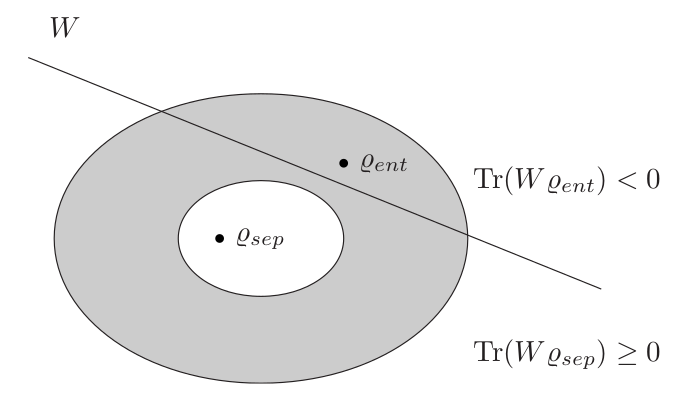
\includegraphics[scale=0.3]{ew.png}
    \end{center}
    \caption{\footnotesize Geometric interpretation of entanglement witnesses. The line represents a hyperplane corresponding to the entanglement witness $W$. All states located to the left of the hyperplane or belonging to it (in particular, all separable states) provide non-negative expctation value of the witness, i.e. $tr(W \rho_{sep}) \geqslant 0$ while those located to the right are entangled states detected by the witness. }
    \label{fig:ew}
\end{figure}

\begin{proof}
The proof of the above theorem goes through the Hahn-Banach theorem which states the following. Consider a sublinear function $\theta : V \longmapsto \Re$ and a linear function $\pi : U \longmapsto \Re$ on the subspace $U \subseteq V$ which is dominated by $\theta$ on $U$, i.e. $\pi (x) \leq \theta (x) \quad \forall x \in U$. There exists a linear extension $\Theta : V \longmapsto \Re$ of $\pi$ to the whole space $V$ such that
\begin{align}
\Theta (x)&=\pi (x) \quad \forall x \in U \\
\Theta (x)& \leq \theta (x) \quad \forall x \in V 
\end{align}
\end{proof}
\subsubsection{Choi-Jamiolkowski isomorphism}
Entanglement witnesses and positive but not completely positive maps are related by the so-called Choi-Jamiolkowski isomorphism \cite{choi}\cite{jamiol}, given by
\begin{equation}
W_{\Lambda}=(\mathbb{I} \otimes \Lambda)\left( \ket{\phi^{+}_d}\bra{\phi^{+}_d}\right)
\end{equation}
where the maximally entangled state $\ket{\phi^{+}_d}\in \mathbb{C}^{d}\otimes \mathbb{C}^d$ is defined as in \autoref{eq:canonical}.
\begin{proof}
Let consider a positive map $\Lambda$ such that $(\mathbb{I} \otimes \Lambda)(\rho)$ yields a non-positive operator, i.e. $\Lambda$ is a not completely positive map. Then 
\begin{equation}
(\mathbb{I} \otimes \Lambda)(\rho)\ket{\chi}=\lambda \ket{\chi}
\end{equation}
where $\lambda < 0$ is a negative eigenvalue of eigenvector $\ket{\chi}$. We can show that observable $W=(\mathbb{I} \otimes \Lambda)(\ket{\chi}\bra{\chi})$ is an entanglement witness. For an arbitrary separable state $\ket{\phi_{sep}}$, we have
\begin{align}
\braket{\phi_{sep}|W|\phi_{sep}}&=tr \left[ \left( (\mathbb{I} \otimes \Lambda)(\ket{\chi}\bra{\chi})\right) \ket{\phi_{sep}}\bra{\phi_{sep}} \right] \\
&= tr \left[ \ket{\chi}\bra{\chi}\left( (\mathbb{I} \otimes \Lambda)(\ket{\phi_{sep}}\bra{\phi_{sep}})\right)  \right] \geqslant 0
\end{align}
where the inequality is due to the positivity of $\Lambda$, such that $(\mathbb{I} \otimes \Lambda)(\ket{\phi_{sep}}\bra{\phi_{sep}})$ is a positive operator. 
\end{proof}

\subsubsection{Optimal entanglement witnesses}
The method of entanglement witnesses is currently considered to be the most important and best
method for detecting entanglement, unfortunately there are infinitely many of them and the determination of entanglement witnesses for all entangled states is a $\mathbb{NP}$-hard problem. 
Constructing entanglement witnesses in general, and finding the minimal set of them that allows for the detection of all entangled states is one of the most challenging open questions.

It is known that the set of quantum states (separable states and entangled states) is convex and compact. Hence, by \autoref{ewtheo} there is at least one "high-level" witness "witnessing" an entanglement witness \cite{optimalEW}. For this high-level witness $\Pi$:
\begin{enumerate}[(i)]
\item $tr(\Pi \rho)\geq 0$ for all quantum (entangled or not) state $\rho$;
\item there exists an entanglement witness $W$ such that $tr(\Pi W)< 0$. 
\end{enumerate}
Operators that satisfy the above two conditions are none other than entangled states. Entanglement witnesses “witness” entangled states and entangled states “witness” entanglement witnesses. Given a "high-level" witness, entangled state $\rho$, we can define $D_{\rho}=\lbrace W | tr(W\rho)<0 \rbrace$, that is the set of operators "witnessed" by $\rho$. Given two entangled states $\rho_1$ and $\rho_2$, we say that $\rho_2$ is finer than $\rho_1$ if $D_{\rho_1}\subseteq D_{\rho_2}$, that is if all the operators “witnessed” by $\rho_1$, are also “witnessed” by $\rho_2$. We say that an entangled state $\rho$ is an optimal high-level witness if there exists no other high-level witness which is finer. 

This leads to a hierarchy of entanglement witnesses. We need a criteria to determine when an EW is optimal \cite{optimalEWKraus}. 
\begin{lemma} Let $W_2$ be finer than $W_1$ and $\delta \equiv \text{inf}_{\rho_1 \in D_{W_1}}\vert \frac{tr(W_2 \rho_1)}{tr(W_1 \rho_1)} \vert$. Then we have:
\begin{enumerate}[(i)]
\item If $tr(W_1 \rho)=0$ then $tr(W_2 \rho) \leq 0$;
\item If $tr(W_1 \rho) < 0$ then $tr(W_2 \rho) \leq tr(W_1\rho)$;
\item If $tr(W_1 \rho) > 0$ then $\delta tr(W_1 \rho) \geq tr(W_2 \rho)$;
\item $\delta \geq 1$, in particular $\delta=1$ if and only if $W_1 =W_2$
\end{enumerate}
\label{lem:w_1}
\end{lemma}
\begin{corollary} $D_{W_1}=D_{W_2}$ if and only if $W_1 =W_2$.
\end{corollary}

An entanglement witness is finer than another one if they differ by a positive operator.  That is, if we have an EW and we want to find another one which is finer, we have to subtract a positive operator

\begin{lemma} An entanglement witness $W_2$ is finer than $W_1$ if and only if there exists a $P$ and $1> \epsilon \geq 0$ such that $W_1=(1-\epsilon)W_2 +\epsilon P$
\label{lem:w_2}
\end{lemma}
By means of the two previuos lemmas we can fully characterize optimal entanglement witnesses.
\begin{theorem} An entanglement witness $W$ is optimal if and only if for all $P>0$ and $\epsilon >0$, $W'=(1+\epsilon)W -\epsilon P$ is not an entanglement witness.
\end{theorem}
\begin{proof}
On the one hand, according to \autoref{lem:w_2} there is no EW which is finier than $W$ and therefore $W$ is optimal. On the other hand, if $W'$ is an EW, then according to the same lemma $W$ is not optimal.
\end{proof}

There exists a class of EW which is very simple to characterize, namely decomposable entanglement witnesses. An entanglement witness $W$ is called decomposable if it can be written in the form
\begin{equation}
W_d = aP + (1-a)Q^{T} 
\end{equation}
where $a\in [0,1]$ and $P,Q \geq 0$. If it does not admit this form it is called non-decomposable. The set of decomposable EW is convex and compact.
\begin{lemma} A decomposable entanglement witness can only detect non-positive partial transpose entangled states.
\end{lemma}
\begin{proof} Consider an entanglement witness $W=P+Q^{T_A}$, then $tr(W\rho)=tr(P\rho)+tr(Q\rho^{T_A})$. Since $P,Q \geq 0$, if $tr(W\rho)<0$ then $\rho^{T_A}\ngeq 0$.
\end{proof}
\begin{theorem} Given a decomposable entanglement witness $W$, if it is optimal then it can be written as $W=Q^T$, where $Q\geq 0$ contains no product vector in its range.
\end{theorem}
\section{Entanglement Measures}
The distinction between separable and entangled states does not allow to compare the amount of entanglement of two different states. For such purpose, we need a quantitative description of entanglement. A way to do that is to consider the interconvertability between quantum states, this is: given two states $\ket{\psi}$ and $\ket{\phi}$, the question is whether or not $\ket{\psi}$ can be transformed into $\ket{\phi}$ by local operations. Consider a bipartite state $\rho$, the most general local operation that acts non-trivially only on the first subsystem reads
\begin{equation}
\rho \longmapsto \sum_{i}(a_i \otimes \mathbb{I})\rho (a^{\dagger}_i \otimes \mathbb{I}), \quad \sum_i a^{\dagger}_i a_i =1
\end{equation}
and analogously for operations on the second subsystem alone. Such operations do not induce any correlations: they map product states on product states,
\begin{equation}
\rho=\rho^A \otimes \rho^B \longmapsto \left( \sum_i a_i \rho^A a^{\dagger}_i \right) \otimes \rho^B
\end{equation}
and separable states on separable states,
\begin{equation}
\rho=\sum_ip_i \rho^{A}_i \otimes \rho^{B}_i \longmapsto \sum_i p_i \left( \sum_j a_j \rho^{A}_j  a^{\dagger}_j \right) \otimes \rho^{B}_i 
\end{equation}
The situation changes if one allows for a correlated application of such local operations, where the operation that is applied at a certain instance depends on the outcomes of previous operations. Such operations are called local operations and classical communication (LOCC). The idea is that Alice and Bob have access to the individual subsystems and they can apply their individual operations to their part of the compositve system. But in order to arrive at the above operation, they would need to communicate with each other, i.e. tell the other one their measurement results via a classical channel. 

LOCC operations can take product states to states no more necessarily of product form. Thus, it is possible to create correlations with LOCC operations, but since these correlations are based on the classical exchange of information, they remain correlations of classical nature. Since LOCC operations are free, i.e. their implementation does not consume entanglement, a state $\ket{\psi}$ which can be mapped into $\ket{\phi}$ by LOCC is necessarily at least as entangled as $\ket{\phi}$. We can define some quantity $E$, called entanglement monotone \cite{EnMon}, that does not increase under LOCC.
$$\ket{\psi} \xrightarrow{\text{LOCC}}\ket{\phi} \Longrightarrow E(\ket{\psi})\geq E(\ket{\phi})$$

Among all LOCC operations, we first consider local unitaries. Consider two bipartite states $\ket{\psi}$ and $\ket{\phi}$, they are LU-equivalent, written $\ket{\psi}\simeq_{LU}\ket{\phi}$, if there exist local unitary operators such that $\ket{\psi}=U_A \otimes U_B \ket{\phi}$. Note that if two states are LU-equivalent they have precisely the same amount of entanglement, and thus they can be usefull for the same applications. 
\begin{equation}
E(\rho) \geq E \left((U_A \otimes U_B) \rho (U^{\dagger}_A \otimes U^{\dagger}_B )\right)
\end{equation}
Because initial and final states are equal, so is their entanglement, and one necessarily concludes that any entanglement monotone is invariant under local unitaries.

\textit{Definition 4.3} \textbf{Entanglement Monotone (EnMon)} A function $E: \mathcal{H}\longmapsto \Re$ is an entanglement monotone if it is non-increasing on average under LOCC,
\begin{equation}
\forall \rho,\lbrace p_i , \sigma_i \rbrace: \rho \xrightarrow{\text{LOCC}} \lbrace p_i , \sigma_i \rbrace \Longrightarrow E(\rho )\geq \sum_i p_i E(\sigma_i})
\end{equation}

\textit{Definition 4.4} \textbf{Entanglement Measure (EnMes)} A function $E: \mathcal{H}\longmapsto \Re$ is an entaglement measure if it is non-increasing under LOCC, i.e. 
\begin{equation}
\forall \rho: \rho \xrightarrow{\text{LOCC}}\Lambda_{LOCC}(\rho) \Longrightarrow E(\rho)\geq E(\Lambda_{LOCC}(\rho))
\end{equation}
The difference between EnMes and EnMon is the final state after the LOCC protocol. In EnMes the final state is clear, is $\Lambda_{LOCC}(\rho)$, but in EnMon the final state is $\sigma_i$ with probability $p_i$. In EnMon, the entanglement cannot increase in average. We see that mathematically there is a difference between entanglement measures and entanglement monotones, EnMon is a stronger condition. 

Examples of entanglement measures are entanglement of formation, concurrence, negativity, Schmidt number, Renyi entropy and so on (see \cite{reviewEM}). Almost all known criteria map an entangled state to a real number (sometimes between 0 and 1 for comparison). Generaly whether a state is regarded as being more entangled than another is dependent on the choice of criterion used. Therefore, there exists the possibility that two different entangled states obtain the same value with respect to
some measure. There also exists the possibility that a criterion indicates $E_1(\rho_1)>E_1(\rho_2)$ but another criterion shows $E_2(\rho_1)<E_2(\rho_2)$.
\subsubsection{Entanglement measures for pure bipartite states}
Invariance under local unitary transformations is not only way to check entanglement monotones as non-monotonous under LOCC, but indeed it has much deeper implications. It implies that any entanglement monotone can be expressed as a function only of invariants under local unitaries.

Consider two pure states $\ket{\psi},\ket{\phi}$. An entanglement measure $E$ for pure states can be define as 
\begin{equation}
\forall \ket{\psi},\ket{\phi}: \ket{\psi} \xrightarrow{\text{LOCC}} \ket{\phi} \Longrightarrow E(\ket{\psi})\geq E(\ket{\phi})
\end{equation}

The Schmidt coefficients introduced in \autoref{theo:schmidt} provide a complete set of invariants, and all entanglement properties can be expressed in terms of them. Consider a pure bipartite state $\ket{\phi}$  such that it can be prepared by LOCC starting from another pure state $\ket{\psi}$. Then, their Schmidt coefficients, ordered decreasingly ($\lambda_1 \geq \lambda_2 \geq \ldots$), satisfy the following inequalities,
\begin{align*}
\lambda^{(\phi )}_1 &\geq \lambda^{(\psi )}_2 \\
\sum^{2}_{i=1}\lambda^{(\phi )}_i &\geq \sum^{2}_{i=1} \lambda^{(\psi )}_i \\
\sum^{3}_{i=1}\lambda^{(\phi )}_i &\geq \sum^{3}_{i=1} \lambda^{(\psi )}_i \\
\vdots & \vdots 
\end{align*}

\begin{theorem}[Majorization] A pure bipartite state $\ket{\phi}$ can be reached from $\ket{\psi}$ by means of LOCC if and only if the majorization condition is fulfilled.
\begin{equation}
\ket{\psi} \xrightarrow{\text{LOCC}} \ket{\phi} \Longleftrightarrow \pmb{\lambda}^{(\phi )} \succeq \pmb{\lambda}^{(\psi )}
\end{equation}
where the Schmidt vectors are $\pmb{\lambda}^{(\phi )}=[\lambda^{(\phi )}_1 , \lambda^{(\phi )}_2 , \ldots ]$ and similarly for $\pmb{\lambda}^{(\psi )}$.
\end{theorem}

Entanglement monotones for pure states can be defined as
\begin{equation}
\forall \ket{\psi},\lbrace p_i,\ket{\phi_i}\rbrace : \ket{\psi} \xrightarrow{\text{LOCC}} \lbrace p_i,\ket{\phi_i}\rbrace \Longrightarrow E(\ket{\psi})\geq \sum_i p_i E(\ket{\phi_i}) 
\end{equation}
Therefore, $E$ is an entanglement monotone for pure states if and only if $E$ is not increasing on average under uni-local operations applied by $A$ and $B$ (we do not need to consider classical communication).

Notice that $\ket{\psi} \xrightarrow{\text{LOCC}} \ket{\phi} = \ket{\psi} \xrightarrow{\text{LOCC}} \lbrace p_1=1,\ket{\phi}\rbrace $, then we can conclude that if $E$ is EnMon for pure states, it is also EnMes for pure states. 


\section{Some applications}
\subsection{Quantum cryptography}
The aim of quantum cryptography is the secure transmission of secret messages from Alice to Bob. The most well known example of quantum cryptography is quantum key distribution, which was first developed by Bennet and Brassard in 1984 \cite{BB84}. In this protocol, known as BB84, Alice want to establish a private key, a sequence of random bits that are only known to Alice and Bob, to transmit a message of the same length to Bob. Single qubits are prepared in non-orthogonal states and then transmitted from A to B and subsequently measured. 
\begin{enumerate}[(i)]
\item Alice randomly selects a bit value $j \in \lbrace 0, 1 \rbrace$ and a basis $\alpha \in \lbrace x,z \rbrace$. She prepares the qubits in the states $\ket{j_\alpha}$, i.e. one of the four states $\lbrace \ket{0},\ket{1},\ket{0_x},\ket{1_x}\rbrace$;
\item Alice sends the qubits to Bob;
\item Bob perfoms a measurement on the qubit in a random basis $\beta \in \lbrace x,z \rbrace$. If $\alpha = \beta$ Bob will obtain a deterministic outcome, otherwise the measurement result is random;
\item Alice and Bob reveal the used bases $\alpha$ and $\beta$ for each qubit through a public channel. If $\alpha = \beta$ they know that they are sharing a random bit $j$;
\item Alice and Bob select randomly M of the bits they share and compare the bit values over the public channel. If many of the bits do not coincide, they assume that an eavesdropper has interfered with the transmission. If all the M bits coincide, the remaining bits can be used as a random bit string, i.e. as a secret key.
\end{enumerate}
The security of the BB84 protocol is based on the fact that any attempt to reveal information about the transmitted quantum system involves the measurement of some observable, it will change the transmitted state and this allows one to detect the presence of an eavesdropper. In addition, it is impossible to clone the state of a single qubit. 

A QKD method based on entangled pairs and Bell's theorem was proposed by Ekert in 1991 \cite{crypto}. The pairs of photons are created by Alice, by Bob, or by some source separated from both of them, and then distributed so that Alice and Bob each end up with one qubit from each pair. Similarly to BB84, the protocol involves a private measurement protocol, Alice measures randomly each photon she receives in some basis set and so does Bob. They keep their series of basis choices private until the measurements are completed. Two groups of qubits are made: the first consists of qubits measured using the same basis and the second contains the rest. To detect eavesdropping, they can compute the correlation coefficients according to Bell's inequalities and check whether Bell's theorem is violated or not. If the protocol is successful, the first group of qubits can be used to generate secure keys since they are completely anti-aligned between Alice and Bob.

The security of E91 relies on the so-called monogamy of entanglement: if two particles are entangled, they will not be entangled to any external system. In other words, no information about the system leaks to environement. If Eve tries to manipulate the qubits the entanglement will be lost.

An interesting fact is that Choi-Jamiolkowski isomorphism shows that prepare-and-measure protocols, such as BB84 and entanglement-based protocols, such as E91 are equivalent.
\subsection{Quantum dense coding}
Quantum dense coding, or superdense coding, was first proposed by Bennet and Weisner in 1992 \cite{densecoding} and it is a quantum communication protocol to transmit two classical bits of information (00, 01, 10, or 11) by first sharing an Bell state between Alice and Bob and then sending only one qubit. Superdense coding is the underlying principle of quantum secret coding since a third particle is unable to get any information without access to both qubits. Superdense conding protocol has the following steps:
\begin{enumerate}[(i)]
\item Alice and Bob share the Bell state $\ket{\phi^{+}}=\frac{1}{\sqrt{2}}(\ket{00}+\ket{11})$;
\item Alice encodes the two classical bits she wants to share by applying a quantum gate to her qubit locally. The four quantum gates are Pauli-gates $\lbrace \mathbb{I},X,Y,Z \rbrace = \lbrace \mathbb{I},\sigma_x ,\sigma_y ,\sigma_z \rbrace $;
\begin{table}[H]
    \centering
    \begin{tabular}{|c|c|c|}
    \hline
   Classical bits & Quantum gate & Resulting Bell state  \\
    \hline
 00 & $\mathbb{I}_{A}$&$\ket{\phi^{+}}$\\
 01& $Z_{A}$&$\ket{\phi^{-}}$\\
 10& $X_{A}$&$\ket{\psi^{+}}$\\
  11& $Z_{A}X_A$&$\ket{\psi^{-}}$\\
   \hline
    \end{tabular}
\end{table}
\item Alice sends her qubit to Bob, and he can make a measurement in the Bell basis and perfectly distinguish whether the state is $\ket{\phi^{+}},\ket{\phi^{-}},\ket{\psi^{+}}$ or $\ket{\psi^{-}}$ since Bell states are orthogonal to each other, and hence retrieve Alice's message. 
\end{enumerate}
In the quantum circuit scheme, a Bell measurement can be seen as a unitary CNOT gate $CNOT^{A \rightarrow B}=\ket{0}^{A}\bra{0}\otimes \mathbb{I}^B + \ket{1}^{A}\bra{1} \otimes \sigma^{B}_x$ followed by a Hadamard gate $H_A \otimes \mathbb{I}_B=\frac{1}{\sqrt{2}}(\sigma_x + \sigma_z)\otimes \mathbb{I}$.

\textsl{\textit{Remark}} There is no contradiction with Holevo's theorem, which states that by using one two-level quantum system, we can only encode 1 bit of classical information. If we count step (i), Alice and Bob exchange 2 qubits in total. More precisely, Alice does not encode her message in an isolated particle, but in a non-locally entangled 2-particle system: not separable into two isolated particles.

\subsection{Teleportation}
As quantum dense coding, teleportation is a quantum communication protocol proposed by Bennet \textit{et al} in 1993 \cite{teleportation}, unless one qubit of information is transmitted instead of two classical bits. Alice can transmit one unknown qubit $\ket{\varphi}=\alpha \ket{0}+ \beta \ket{1}$ to Bob by first sharing a Bell state, which is used as a perfect quantum channel, and then locally manipulating her qubit and sending classical information. Teleportation protocol has the following steps:
\begin{enumerate}[(i)]
\item Alice and Bob share the Bell state $\ket{\phi^{+}}=\frac{1}{\sqrt{2}}(\ket{00}_{AB}+\ket{11}_{AB})$, Alice has an extra qubit to be teleported $\ket{\varphi}$, so the initial state is $\ket{\varphi}\ket{\phi^{+}}$;
\item Alice makes a local Bell measurement on her two qubits $A',A$, the resulting state is 
\begin{align*}
\frac{1}{\sqrt{2}}\left(\ket{00}_{A'A}(\alpha \ket{0}_{B}+ \beta \ket{1}_{B})+ \ket{01}_{A'A}(\alpha \ket{1}_{B}+ \beta \ket{0}_{B}) \\ + \ket{10}_{A'A}(\alpha \ket{0}_{B}- \beta \ket{1}_{B}) + \ket{11}_{A'A}(\alpha \ket{1}_{B}- \beta \ket{0}_{B}) \right)
\end{align*}
\item Alice makes a measurement in the computational basis on her two qubits and she tells Bob the resulting state using a classical channel;
\item According to Alice's message, Bob applies a correction operation on qubit $B$ and he obtains the desired state $\ket{\varphi}$.

\begin{table}[H]
	\centering
	\begin{tabular}{|c|c|}
	\hline
	Alice's result & Correction \\
	\hline
	$\ket{00}$ & $\mathbb{I}_B$\\
	$\ket{01}$ & $X_B$\\
	$\ket{10}$ & $Z_B$\\
	$\ket{11}$ & $Z_{B}X_{B}$\\
	\hline
	\end{tabular}
\end{table}
\end{enumerate}

Notice that qubit $B$ takes over completely the role of qubit $A'$, in particular also its entanglement with additional particles. This property can be used for entanglement swapping, where entanglement between systems $AC_1$ and $C_2 B$ leads to an entanglement state between systems $AB$ by teleporting $C_1$ to $B$. Teleportation has been experimentally demonstrated for single photons \cite{teleportphotons}, light beams \cite{teleportbeams}, atoms \cite{teleportatoms} and also between light and matter \cite{teleportmatter}.

\chapter{Quantum Communication} \label{chap:QN}
Quantum communication is one of the most advanced applications of quantum information processing, and a basic tool for distributed quantum computation or quantum cryptography, where the transmission of quantum states allows one to establish a secret key between two communication partners, enabling secure communication. For all these applications of a quantum communication network, the term quantum internet has been suggested \cite{QI}, in analogy with the classical internet. In classical communication, to send a message means to correlate the sender to the receiver. Thus the ability to faithfully transmit a bit is equivalent to the ability to faithfully share maximally correlated bits. In quantum communication theory it is entanglement which will play the role of correlations, and for this reason entanglement is the key tool of quantum communication theory. To send quantum information is equivalent to transmit an unknown entangled quantum state \cite{teleportation}. 

However, for quantum communication, teleportation alone is not sufficient. If we send maximally entangled states through a noisy quantum channel we end up with noisy, non-maximally entangled states, and although they can still be used for quantum teleportation, the fidelity of the teleported qubits is reduced. The generation and maintenance of high-fidelity entanglement is a central problem, noisy operations as well as interactions with the environement have the effect that the desired entangled states are produced only with a certain non–unit fidelity. In aim to solve the problem of quantum communication over noisy quantum channels several methods have been designed in last years.

Although classical communication theory inspires techniques for quantum communication, there are several issues that need to be considered. First, coding based on data-copying, which is used in classical error correction cannot be used due to the no-cloning theorem of quantum mechanics. This result implies that there exists no transformation resulting in the following mapping,
\begin{equation}
U(\ket{\psi}\otimes \ket{e})= \ket{\psi}\otimes \ket{\psi} \quad \forall \ket{\phi}
\end{equation}
i.e. it is impossible to perfectly copy an unknown quantum state.
\begin{proof} Assume that such general transformation $U$ exists. Take and arbitray state $\ket{\chi}$ and consider
\begin{align}
(\bra{\chi}\otimes \bra{e})( \ket{\psi}\otimes \ket{e}) &= \braket{\chi|\psi}\braket{e|e}\\
(\bra{\chi}\otimes \bra{e})U^{\dagger}U( \ket{\psi}\otimes \ket{e}) &= (\bra{\chi}\otimes \bra{\chi})( \ket{\psi}\otimes \ket{\psi})\\
&= \vert \braket{\chi |\psi}\vert^{2}
\end{align}
So $\braket{\chi|\psi}=\vert \braket{\chi |\psi}\vert^{2}$, therefore they are either the same state or $\braket{\chi |\psi}=0$
\end{proof}
This means that quantum data cannot be protected from errors by simply making multiple copies. Secondly, direct measurement cannot be used to effectively protect against errors, since this will destroy any quantum superposition. Two solutions are proposed:
\begin{enumerate}[(i)]
\item quantum error correction: the information is encoded in a larger dimensional Hilbert space and it is protected from noise.
\item entanglement purification (combined with teleportation): the information is transmitted by means of teleportation, using a known entangled state with sufficiently high fidelity which is obtained by entanglement purification.
\end{enumerate}
\section{Quantum Error Correction}
Quantum error correction codes utilizes the idea of redundant encoding. The total size of the Hilbert space is expanded beyond what is needed to store a single qubit of information, and in this way, errors on individual qubits are mapped to large set of mutually orthogonal subspaces, the size of which is determined by the number of qubits utilized in the code. In quantum error correction codes, quantum information is protected by encoding one logical qubit of information into several physical qubits, or more generally $k$ logical qubits into $n$ physical qubits. In the simplest case where one qubit is encoded into $n$ qubits, we define the logical qubits $\ket{0_L},\ket{1_L}$ as two orthogonal states in $\mathbb{C}^{2n}$. Any entangled state $\alpha \ket{0}+\beta \ket{1}$ is encoded via unitary encoding operation yielding an encoded state
\begin{equation}
(\alpha \ket{0}+\beta \ket{1})\otimes \ket{0}^{\otimes n-1} \rightarrow \alpha \ket{0_L}+\beta \ket{1_L}
\end{equation}
Logical qubits $\ket{0_L},\ket{1_L}$ span a two-dimensional subspace which is mapped to orthogonal two-dimensional subspaces by error operators. Then by measuring appropriate two–dimensional projectors, one can distinguish between these subspaces and correct the errors. If all the subspaces are pairwise orthogonal then the corresponding code is able of an independent treatment of errors and of correcting all of them. Importantly, coherent superpositions within each of the subspaces are not altered and hence quantum information is preserved. 

Finally, the error correction protocol cannot allow us to gain information regarding the coefficients, $\alpha$ and $\beta$ of the encoded state since that would collapse the system.

Unlike classical information, qubits are susceptible to both bit-flip errors $\ket{0}\leftrightarrow \ket{1}$ and phase-flip errors $\ket{0}\leftrightarrow \ket{0}$, $\ket{1}\leftrightarrow -\ket{1}$. Hence, any error correction procedure needs to be able to simultaneosusly correct for both. 

\subsection{The 9-qubit code}
The 9-qubit error correcting code was first developed by Shor in 1995 \cite{shor}, demonstrating that QEC was possible. The Shor code is a degenerate single error correcting code, i.e. different types of errors have the same syndromes, and it is able to correct a logical qubit from one bit-flip, one phase-flip or one of each, on any of the nine physical qubits. This code is therefore sufficient to correct for an arbitrary single qubit error.

The two basis states for the code are,
\begin{align}
\ket{0_L}&=\frac{1}{\sqrt{8}}(\ket{000}+\ket{111})(\ket{000}+\ket{111})(\ket{000}+\ket{111})\\
\ket{1_L}&=\frac{1}{\sqrt{8}}(\ket{000}-\ket{111})(\ket{000}-\ket{111})(\ket{000}-\ket{111})
\end{align}
and the circuit to perfom the encoding is shown in \autoref{fig:9QEC}. 
\begin{figure}[H]
    \begin{center}
        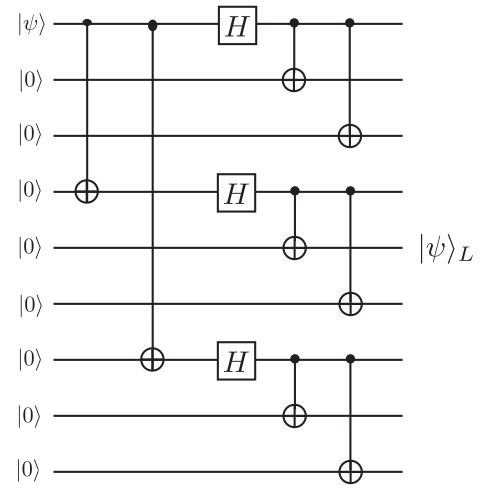
\includegraphics[scale=0.3]{9qubitQEC.png}
    \end{center}
    \caption{\footnotesize Circuit required to encode a single qubit with 9-qubit code.}
    \label{fig:9QEC}
\end{figure}

For single bit-flip errors $\sigma_x \equiv X$ we consider blocks of three qubits, i.e. $\ket{0_L}=\ket{000}$ and $\ket{1_L}=\ket{111}$ such that an arbitrary single qubit state $\ket{\psi}=\alpha \ket{0}+\beta \ket{1}$ is mapped to
\begin{align*}
\alpha \ket{0}+\beta \ket{1} & \rightarrow \alpha \ket{0_L}+\beta \ket{1_L}\\
&= \alpha \ket{000}+\beta \ket{111}\\
&=\ket{\psi_L}
\end{align*}
For each block of three qubits encoded to $(\ket{000}+\ket{111})/ \sqrt{2}$ we perfom the correction circuit shown in \autoref{fig:XQEC}, we assume that all gate operations are perfect. Correction proceeds by introducing two ancilla qubits and performing a sequence of CNOT gates, which checks the parity of the three qubit data block. Using syndrome information, the $X$ error can be corrected with a classically controlled $\sigma_x$ gate. Phase-flip errors $\sigma_z \equiv Z$ can be corrected by checking the sign differences between the three blocks of qubits.
\begin{figure}[H]
    \begin{center}
        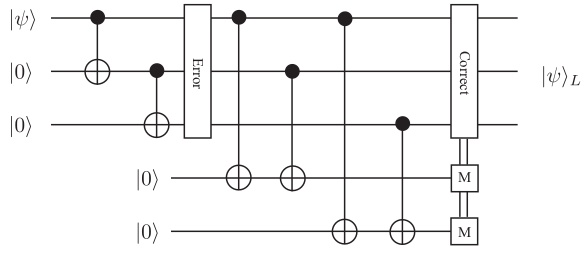
\includegraphics[scale=0.4]{XerrorQEC.png}
    \end{center}
    \caption{\footnotesize Circuit for encode and correct single $X$ errors. After encoding a single logical qubit via two ancilla qubits and two CNOT gates, two extra ancilla qubits are coupled to the data block. These ancilla are measured and the measurement result indicates if an error has ocurred and where.}
    \label{fig:XQEC}
\end{figure}
For each possible situation, either no error or a single bit-flip error, the ancilla qubits are flipped to a unique state based on the parity of the data block. These qubits are then measured to obtain the classical syndrome result and the result of the measurement will indicate if a correction is needed.
\begin{table}[H]
    \centering
    \begin{tabular}{|c|c|c|}
    \hline
   Ancilla measurement & Collapsed state & Error \\
    \hline
   00 &$\alpha \ket{000}+\beta \ket{111}$& No error \\
   01 &$\alpha \ket{001}+\beta \ket{110}$& $\sigma_x$ on qubit 3 \\
   10 &$\alpha \ket{010}+\beta \ket{101}$& $\sigma_x$ on qubit 2 \\
   11 &$\alpha \ket{100}+\beta \ket{011}$& $\sigma_x$ on qubit 1 \\
    \hline
    \end{tabular}
	\caption{\footnotesize Ancilla measurements for single $\sigma_x$ error for a block of three qubits. Each of the four possible results correspond to either no error or a bit flip on one of the three qubits.}
	\label{tab:xerror3}
\end{table}
The distance between two codeword states, $d$, defines the number of errors that can be corrected, $t$, as, $t = (d − 1)/2$. In this case, for each block of three qubits we have $d=3$, hence $t=1$. This code will only work if a maximum of one error occurs per block.
\begin{table}[H]
    \centering
    \begin{tabular}{|c|c|c|}
    \hline
   Error & Final state: data, ancilla & Assumed error \\
    \hline
   Qubits 1,2 &$\alpha \ket{110}\ket{01}+\beta \ket{001}\ket{01}$& $\sigma_x$ on qubit 3  \\
   Qubits 2,3 &$\alpha \ket{011}\ket{11}+\beta \ket{100}\ket{11}$& $\sigma_x$ on qubit 1  \\
   Qubits 1,3 &$\alpha \ket{101}\ket{10}+\beta \ket{010}\ket{10}$& $\sigma_x$ on qubit 2 \\
   Qubits 1,2,3 &$\alpha \ket{111}\ket{00}+\beta \ket{000}\ket{00}$& No error  \\
    \hline
    \end{tabular}
	\caption{\footnotesize Error syndromes are not unique when multiple errors occur.}
	\label{tab:errorsyndromes}
\end{table}
Notice that a phase-flip on any one qubit in a block of three has the same effect, this is why 9-qubit code is a degenerate code. In other error correcting codes, such as the 5- or 7-qubit codes (\cite{5qec}, \cite{7qec}), there is a one-to-one mapping between errors and unique states. In degenerate codes such as the 9-qubit code, the mapping is not unique, we know in which block the error occurs and it does not matter which qubit we apply the correction operator to. As the 9-qubit code can correct for a single $X$ error in any one block of three and a single phase-flip error on any of the nine qubits, this code is a full quantum error correcting code. However, in general, the 9-qubit code is only a single error correcting code as
it cannot handle multiple errors if they occur in certain locations.

\subsection{QEC with stabilizer codes}
The use of the stabilizer formalism introduced in the context of grah states in                                                                                 
 \autoref{sec:Stabilizer} to describe quantum error correction codes is very useful since it allows easy generalised representation of correction circuits, regardless of the code used \cite{Gottesman}.
A state $\ket{\psi}$ is defined to be stabilized by operator $K$ if it is an eigenstate of $K$ with eigenvalue +1,
\begin{equation}
K\ket{\psi}=\ket{\psi}
\end{equation}
For example, the single qubit state $\ket{0}$ is stabilized by operator $K=\sigma_x$, i.e. $\sigma_x \ket{0}=\ket{0}$.

The association between stabilizer codes and stabilizer states comes about by defining a coding subspace. Consider a bipartite state $\ket{\psi}\in \mathbb{C}^2 \otimes \mathbb{C}^2$, the Hilbert space has dimension four, however if we require that this two qubit state is stabilized by $\sigma_x \otimes \sigma_x \equiv XX$, then there are only two orthogonal basis states which satisfies that,
\begin{align}
\ket{0_L}&=\frac{1}{\sqrt{2}}(\ket{01}+\ket{10})\\
\ket{1_L}&=\frac{1}{\sqrt{2}}(\ket{0}+\ket{11}
\end{align}
Hence by using stabilizers we can reduce the size of the Hilbert space for a multi-qubit system to an effective single qubit system. For a $n$-qubit system the Hilbert space has dimensionality $2^n$, if the stabilizer set of this system contains $k$ elements then the dimension of the subspace is $2^{n-k}$. A stabilizer code is therefore a subspace defined via stabilizer operators for a multi-qubit system containing $n-k$ logical qubits.

Consider the 9-qubit code, its stabilizer set is fully specified by the eight following operators
\begin{align*}
K^1 = ZZIIIIIII \quad &\quad K^5 = IIIIII ZZI \\
K^2= Z I Z IIIIII \quad &\quad K^6 = IIIIIII Z I Z \\
K^3 = III ZZ IIII \quad &\quad K^7 = XXXXXXIII \\
K^4 = III Z I Z III \quad &\quad K^8 = XXX III XXX \\
\end{align*}
The dimensionality of a 9-qubit system is $2^9$ and there are eight stabilizers, therefore the total dimension of this subspace defined by the stabilizer set is $2^{9-8}=2$. The stabilizer set now defines an effective 2-dimensional subspace, and it encodes nine physical qubits into one logical qubit t correct for a single $X,Z$ error. When we measure the eigenvalue of $K^1$, we determine if a bit-flip error has happened on qubit one or two, i.e. if $\sigma^{(1)}_x$ or $\sigma^{(2)}_x$ has happened. Note that both of these errors anticommute with $K^1$, while $\sigma^{(3)}_x$ through $\sigma^{(9)}_x$, which cannot be detected by just $K^1$, commute with it. Similarly, $K^2$ detects $\sigma^{(1)}_x$ or $\sigma^{(3)}_x$, which anticommute with it, and $K^7 $detects $\sigma^{(1)}_z$ through $\sigma^{(6)}_z$. 


\subsection{Quantum error detection}
We have focused on the requirement not only to detect errors but also correct them, however another approach is to not force the correcting ability. Post-selected quantum computation \cite{Kni05} demonstrated that large scale quantum computing could be achieved with higher noise rates when only error detection is used instead of more costly error correction codes. In general, error detection is faster and requires fewer qubits than performing active error correction, but on the other hand the resource requirements are much higher.

For error detection, it is only require that an error operator $O_j$ maps states within subspace $S$ to orthogonal subspace $S^\bot$, but it is not necessary that subspaces of different error operators
are pairwise orthogonal. This implies that different error operators can lead to the same output state, and hence are indistinguishable.

The basic idea in post-selected schemes is to encode a large number of ancilla qubits with error detecting circuits, then  sets of encoded qubits which pass error detection are selected and utilized as encoded ancillas for error correction. By producing and verifying large numbers of encoded ancillas which are post-selected, error correction can be performed without data qubits waiting as long for appropriate ancilla to be prepared, decreasing the number of errors that need to be corrected.

\section{Entanglement Purification}

When distant parties share $n$ copies of a mixed state $\rho$, which contains noisy entanglement, they can perform some LOCC, i.e. a sequence of local operations and one or two-way classical communication and obtain a reduced number of $k$ pairs with increase fidelity. A sequence of LOCC operations achieving this task is called entanglement purification or entanglement distillation protocol. In entanglement purification, several copies of noisy, non–maximally entangled states are manipulated in such a way that a fewer number of copies with a reduced amount of noise are produced. This is possible since the desired state is known. The entanglement of the total ensemble is concentrated or distilled in a few copies, which hence contain a larger amount of entanglement and have higher fidelity, entanglement is purified at the cost of obtaining smaller number of copies. After purification protocol, the distilled states can be used to perfom quantum teleportation, quantum cryptography or other entanglement-based protocols. 

Entanglement purification protocols were first introduced for bipartite states \cite{EPbi}, and later for multipartite entangled states, in particular graph states or stabilizer states \cite{EPgraph}, \cite{EPandQEC}, \cite{MultiEPGS}, \cite{EPtwocolor}. In the multipartite case, there is no distinguished state like a singlet state that can be a universal target state in entanglement distillation procedures, however there are some classes of interesting target states, including the commonly studied GHZ state. 

Purification protocols differ in the number of copies of the states they operate on and they can purify, the efficiency, and also whether they allow one-way or two-way classical communication. Consider a protocol that operates on $N$ copies of noisy entangled states and produce $M\leq N$ purified copies. In case of one–way classical communication $A \rightarrow B$, we measure $N - M$ copies and use the obtained information to choose a proper correction operation on the remaining pairs. Notice that for the choice of these correction operations, Alice only has access to the local measurement outcomes in $A$, while Bob has access to outcomes of measurements in $A$ and $B$. In particular, this implies that the particles cannot decide to discard certain pairs based on joint measures outcomes. To make this possible, two-way classical communication is needed. The purification protocols can be grouped into distillation protocols, where an ensembre of many copies is manipulated to get a few pairs with higher fidelity; and recurrence and pumping schemes, which are based on the iteration of a purification step several times, resulting in pairs with improved fidelity.

We define the yield of a EP protocol for quantitying how efficient a protocol is. Consider some $N\rightarrow M$ protocol, i.e. a protocol which starts with $N$ copies of a mixed state, $\rho^{\otimes N}$ and after purification $M$ copies of a maximaly entangled state are obtained. The yield of the protocol with respect to the state $\rho$ is defined as
\begin{equation}
Y_\rho = \frac{M}{N}
\end{equation}
We are interested in optimal entanglement purification protocols, i.e. those which result in a maximal ratio $M/N$. More precisely, we demand that for all $\epsilon > 0$, the fidelity of the resulting state after puritication protocol with respect to $M$ copies of a maximally entangled state $\ket{\Phi}=\ket{\phi^+}^{\otimes M}$ must be $F \geq 1-\epsilon$. The yield is then determined by the ratio $M/N$ of the maximum $M$ for which this is the case in the asymptotic limit of $N \rightarrow \infty$. This optimal ratio is called distillable entanglement and denoted as $E_D$.
Notice that such a strict definition of yield actually implies that many entanglement purification protocols have zero yield, although they can produce entangled states with arbitrary high fidelity.

The purification range of a protocol is defined as the set of all input states $\rho$ that can be purified by the protocol, i.e. where maximally entangled states can be generated from $N$ copies of $\rho$ in the asymptotic limit of $N \rightarrow \infty$.
\subsection{Basic purification protocols}

\subsection{Bound entanglement}
The distillability problem, i.e. the question whether there exists a LOCC protocol that can generate maximally entangled states from (infinitely) many copies of a state, has been extensively studied in recent years, however a complete solution has not been obtained so far. What is, however, known are necessary conditions for distillability (e.g. that the partial transposition of the density operator is non–positive), as well as sufficient criteria.

A question fundamental for quantum information processing then immediately arose: Can noisy entanglement always be purified? Bound entanglement vs free entanglement (can be distilled)

\subsection{Error model}
We consider entanglement purification protocols under non–idealized conditions, i.e. local operations are noisy. The main effect of noise is that no longer maximally entangled states can be produced, and the achievable fidelity is smaller than unity. Similarly, the required initial fidelity in the case of noisy local control operations is larger. We describe a noisy single-qubit operation by $\hat{U}\prod_{k}\varepsilon^{(k)}_{q}\rho$, i.e. single-qubit local noise with error parameter $q$, followed by the perfect unitary operation $\hat{U}$ with $\hat{U}\rho = U \rho U^{\dagger}$. We model local noise by
\begin{equation}
\varepsilon^{(k)}_{q}\rho = U_{k} [\mathcal{M}_k \mathcal{M}_k \rho]U^{\dagger}_{k}
\end{equation}
where $\mathcal{M}_k$ is a local completely positive maps, which may denote white noise (depolarizing channels),
\begin{equation}
\mathcal{M}_k \rho = q\rho + (1-q)\frac{1}{4}\sum^{3}_{i=0}\sigma^{(k)}_{i}\rho \sigma^{(k)}_{i}
\end{equation}
bit-flip channels,
\begin{equation}
\mathcal{M}^{B}_k \rho = q\rho +(1-q)\frac{1}{2}(\rho +\sigma^{(k)}_{1}\rho \sigma^{(k)}_{1} )
\end{equation}
and phase-flip channels (dephasing channels),
\begin{equation}
\mathcal{M}^{P}_k \rho = q\rho +(1-q)\frac{1}{2}(\rho +\sigma^{(k)}_{3}\rho \sigma^{(k)}_{3} )
\end{equation}

\section{Quantum Repeater}

For long-distance quantum communication, entanglement purification alone is not sufficient, losses and noise increase exponentially with the distance, thereby limiting the maximal distance to a few hundred kilometers when using photons transmitted through optical fibers. For this reason, in order to achieve the vision of secure quantum communication over arbitrary distances, several schemes have been proposed 
which either utilize quantum error correction or combine entanglement purification and entanglement swapping, thereby generating high fidelity entangled pairs that can then be used to teleport arbitrary quantum information. Similar to classical communication approach, such schemes can be seen as quantum repeaters. 

The basic idea behind quantum repeaters is to split the long channel into smaller segments, and generate short-distance entangled pairs that are purified later to some fidelity $F_0$. These short-distance pairs are then connected via Bell measurements, which is equivalent to an entanglement swapping, to form an entangled pair of longer distance. For noisy operations, the fidelity of the resulting pairs is reduced, and only a few can be connected in this way. One then uses entanglement purification to re-purify these mid-distance pairs to the working fidelity $F_0$. When applied to all segments simultaneously, this leaves us with the same situation as initially, except that the distance of the pairs is enlarged. This procedure can than be applied in a nested way, thereby always at least doubling the distance. The required resources, i.e. the number of elementary pairs, increase only polynomial with the distance \cite{QR98}.


Quantum communication between distant parties is based on suitable instances of shared entanglement. For
efficiency reasons, in an anticipated quantum network beyond point-to-point communication, it is preferable that many parties can communicate simultaneously over the underlying infrastructure. Sharing of multi-partite entangled states between parties offers a solution, allowing for parallel quantum communication. Specifically for the two-pair problem, the butterfly network provides the first instance of such an advantage in a bottleneck scenario. The underlying method differs from standard repeater network approaches in that it uses a graph state instead of maximally entangled pairs to achieve long-distance simultaneous communication. 


As we have seen, the quantum repeater is a scheme that allows for efficient long-distance quantum communication. In a real-world application of quantum communication such as a quantum internet \cite{QI}, one deals with a multi-user communication network. The network has to be able to establish high-fidelity long-distance entangled pairs between the nodes but also it has to allow flexible communication between all the partners. Hence, to ensure multi-user communication, any given pair of particles has to be able to share entanglement and communicate to each other. For this purpose, 1D networks are not sufficient since they can only establish bipartite communication. In \cite{twodim}, Dür \textit{et al} proposed a 2D quantum repeater 



\section{Two-dimensional quantum repeater}


\begin{figure}[H]
    \begin{center}
        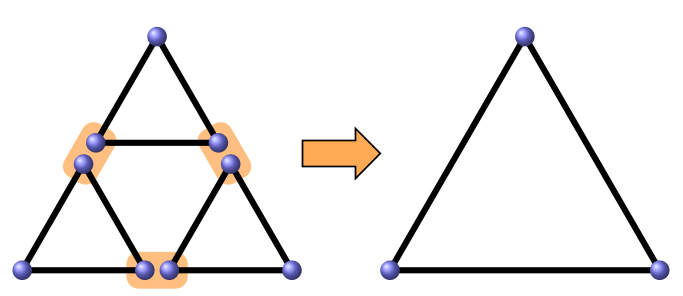
\includegraphics[scale=0.3]{CoarseGHZ3.png}
    \end{center}
    \caption{\footnotesize 2D repeater architecture based on three-particle GHZ states. Three short-distance GHZ states are connected to form one long-distance GHZ with reduced fidelity. Image taken from \cite{twodim}.}
    \label{CGHZ3}
\end{figure}

\begin{equation}
\frac{1}{\sqrt{2}}(\ket{000}+\ket{111})\otimes \frac{1}{\sqrt{2}}(\ket{000}+\ket{111})\otimes \frac{1}{\sqrt{2}}(\ket{000}+\ket{111})
\end{equation}

The protocol can be summarized as follows:
\begin{enumerate}
\item Start with three copies of a (probably noisy) GHZ state.
\item Perfom Bell measurements on labeled qubits (2,6), (3,8), (5,9) (see \autoref{GHZ3}) 
\item Depending on the outcomes of the Bell measurements, perform correction operations on remaining qubits 1,4 and 7.
\end{enumerate}

The resulting state after performing Bell measurements I, II, III on qubits (2,6), (3,8) and (5,9), respectively is:
\begin{align}
  (\ket{000}+\ket{111})\otimes \ket{\phi^{\pm}}\otimes \ket{\phi^{\pm}}\otimes \ket{\phi^{\pm}} \\
+ (\ket{001}+\ket{110})\otimes \ket{\phi^{\pm}}\otimes \ket{\psi^{\pm}}\otimes \ket{\psi^{\pm}} \\
+ (\ket{010}+\ket{101})\otimes \ket{\psi^{\pm}}\otimes \ket{\phi^{\pm}}\otimes \ket{\psi^{\pm}} \\
+ (\ket{100}+\ket{011})\otimes \ket{\psi^{\pm}}\otimes \ket{\psi^{\pm}}\otimes \ket{\phi^{\pm}} 
\end{align}
Therefore, 
\begin{table}[H]
    \centering
    \begin{tabular}{|c c c|c|}
    \hline
    Bell I & Bell II & Bell III & Correction \\
    \hline
    $\phi^{\pm}$&$\phi^{\pm}$&$\phi^{\pm}$&$\mathbb{I}$\\
    $\psi^{\pm}$&$\psi^{\pm}$&$\phi^{\pm}$&$X^{(1)}$\\
    $\psi^{\pm}$&$\phi^{\pm}$&$\psi^{\pm}$&$X^{(4)}$\\
    $\phi^{\pm}$&$\psi^{\pm}$&$\psi^{\pm}$&$X^{(7)}$\\
    \hline
    \end{tabular}
	\caption{\footnotesize Table of corrections for the four different measurements patterns.}
	\label{tab:NOerror}
\end{table}

Notice that we only need two of the three Bell measurements to connect the three GHZ states. The third measurement does not only make the protocol symmetric but can actually be used to detect some specific errors. As it will be described below, error syndromes are not unique and therefore it is not possible to correct the errors detected but it allows us to discard the cases with errors and obtain better error thresholds. However, this also means that the connection procedure only works probabilistically, and the whole procedure has to restart from the beginning if errors are detected.

\begin{figure}[H]
    \begin{center}
        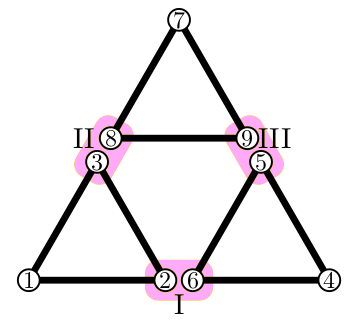
\includegraphics[scale=0.4]{GHZ3.png}
    \end{center}
    \caption{\footnotesize Repeater scheme connecting protocol based on Bell measurements.}
    \label{GHZ3}
\end{figure}

We can distinguish two sets of qubits: qubits not involved in Bell measurements $\lbrace 1,4,7 \rbrace$, which remain in the next level of the quantum repeater and qubits involved in Bell measurements $\lbrace 2,3,5,6,8,9 \rbrace$ which vanish. To carry out the error handling procedure we consider only single-qubit errors: bit-flip errors or error in $x$-basis, phase-flip errors or error in $z$-basis and combination of both. 

Consider a bit-flip error in the set of qubits $\lbrace 1,4,7 \rbrace$.
\begin{table}[H]
    \centering
    \begin{tabular}{|c c c|c|c|c|}
    \hline
    Bell I & Bell II & Bell III & Error in 1 & Error in 4 & Error in 7 \\
    \hline
  $\phi^{\pm}$&$\phi^{\pm}$&$\phi^{\pm}$&$X^{(1)}$&$X^{(4)}$ &$X^{(7)}$\\
  $\psi^{\pm}$&$\psi^{\pm}$&$\phi^{\pm}$&$X^{(1)}$&$X^{(4)}$ &$X^{(7)}$\\
  $\psi^{\pm}$&$\phi^{\pm}$&$\psi^{\pm}$&$X^{(1)}$&$X^{(4)}$ &$X^{(7)}$\\
  $\phi^{\pm}$&$\psi^{\pm}$&$\psi^{\pm}$&$X^{(1)}$&$X^{(4)}$ &$X^{(7)}$\\
    \hline
    \end{tabular}
	\caption{\footnotesize Table of corrections for a bit-flip error in qubits located at 1,4 or 7.}
	\label{tab:Error147}
\end{table}
Therefore, we see that not only the error syndromes are the same but they coincide with the measurement results with no error(see \autoref{tab:NOerror}). We cannot distinguish between the Bell measurements pattern, either there is no error or one bit-flip error and if we apply one of the correction operations there is a probability of $\frac{1}{4}$ of success.

Now, we consider a bit-flip error in connection qubits. First, despite there are 6 remaining qubits, measurement patterns are the same for the two qubits involed in the same Bell measurement, then we only need to consider three different cases.
\begin{table}[H]
    \centering
    \begin{tabular}{|c c c|c|c|c|}
    \hline
   Bell I & Bell II & Bell III & Error BM I & Error BM II & Error BM III \\
    \hline
  $\psi^{\pm}$&$\phi^{\pm}$&$\phi^{\pm}$&$\mathbb{I}$&$X^{(1)}$&$X^{(4)}$ \\
  $\phi^{\pm}$&$\psi^{\pm}$&$\phi^{\pm}$&$X^{(1)}$&$\mathbb{I}$&$X^{(7)}$ \\
  $\phi^{\pm}$&$\phi^{\pm}$&$\psi^{\pm}$&$X^{(4)}$&$X^{(7)}$&$\mathbb{I}$\\
  $\psi^{\pm}$&$\psi^{\pm}$&$\psi^{\pm}$&$X^{(7)}$&$X^{(4)}$ &$X^{(1)}$\\
   \hline
    \end{tabular}
	\caption{\footnotesize Table of corrections for a bit-flip error in qubits located at (2,6), (3,8) and (5,9).}
	\label{tab:errorI}
\end{table}   
Error syndromes are the same, for each measurement outcome there is a set of three correction operations, therefore if we apply one of the correction operations there is a probability of $\frac{1}{3}$ of success.


\begin{figure}[H]
    \begin{center}
        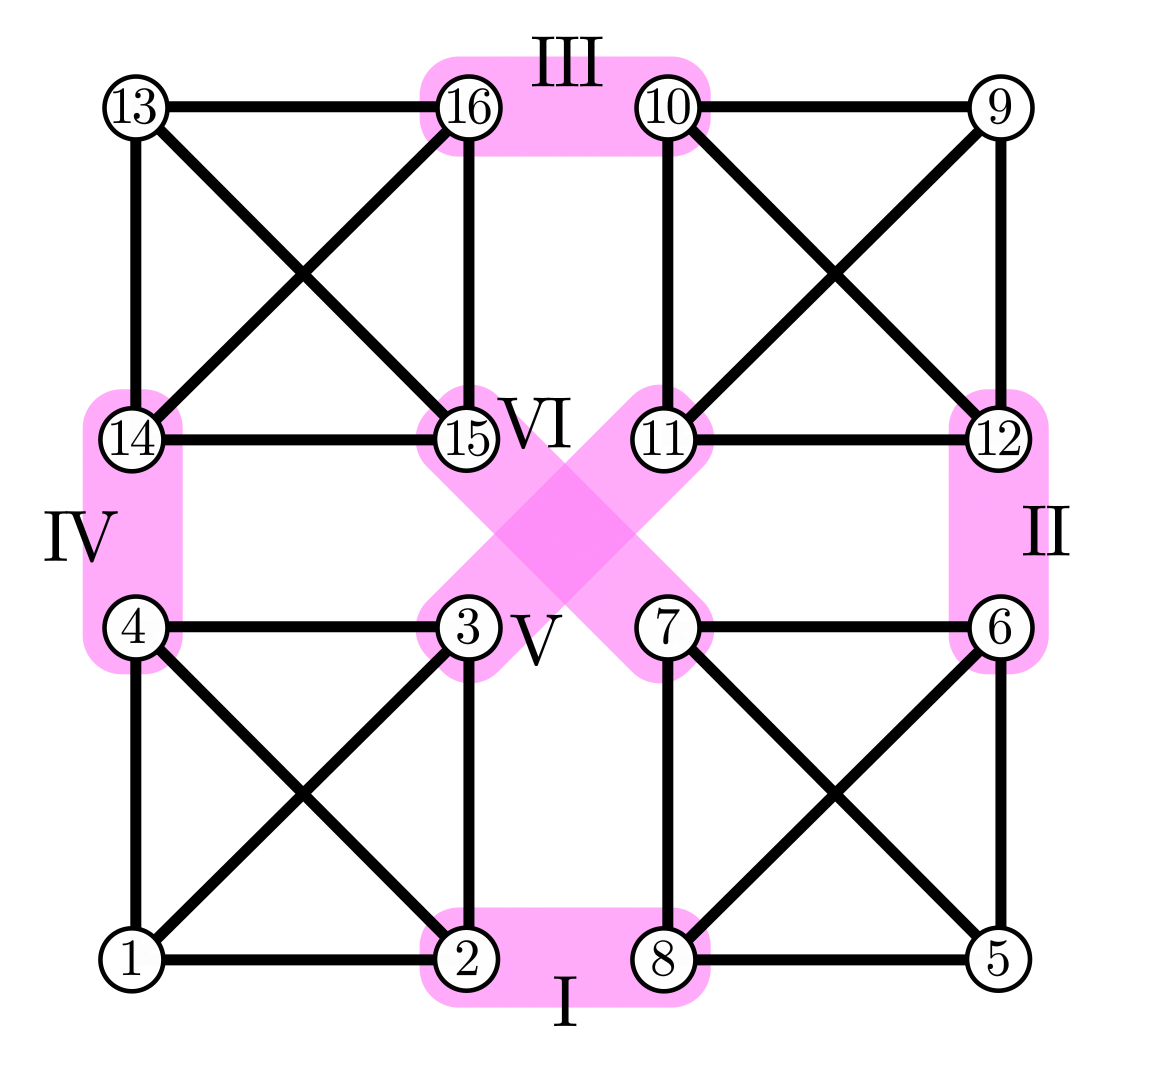
\includegraphics[scale=0.2]{GHZ4.png}
    \end{center}
    \caption{\footnotesize Repeater scheme using four GHZ states of four particles.}
    \label{GHZ4}
\end{figure}


\begin{figure}[H]
    \begin{center}
        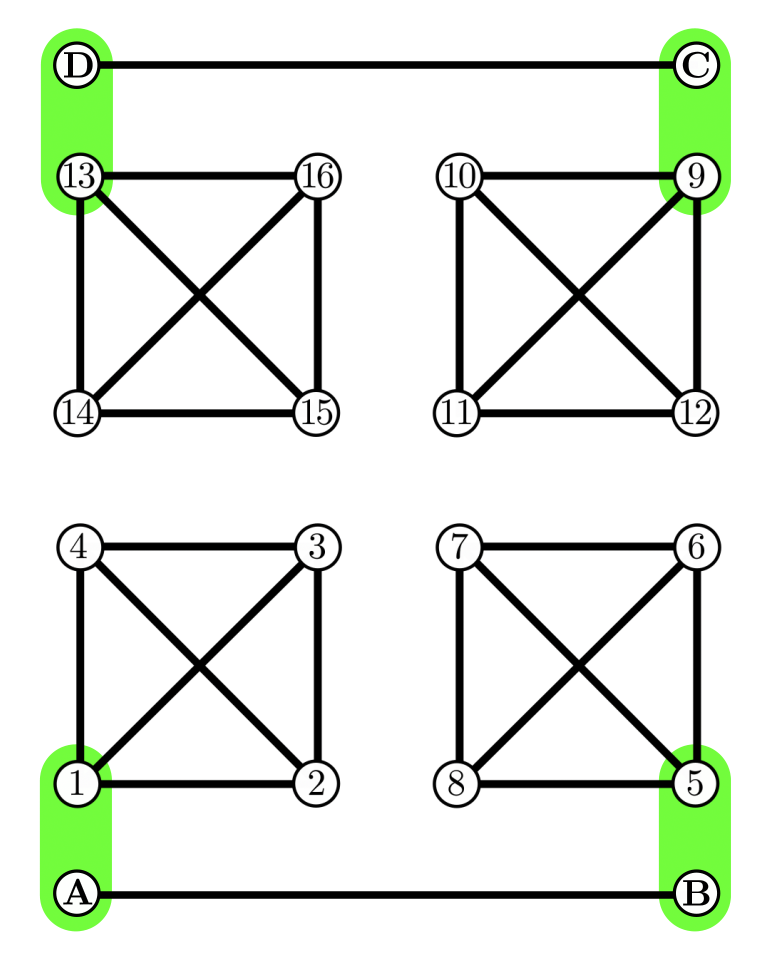
\includegraphics[scale=0.3]{GHZ4Bell.png}
    \end{center}
    \caption{\footnotesize .}
    \label{GHZ4Bell}
\end{figure}








\pagebreak


\begin{appendices}

\chapter{Tables GHZ4}

\begin{table}[H]
    \centering
    \begin{tabular}{|c c c c c c|c|}
    \hline
   Bell I & Bell II & Bell III & Bell IV & Bell V & Bell VI & Correction  \\
    \hline
  $\phi^{\pm}$&$\phi^{\pm}$&$\phi^{\pm}$&$\phi^{\pm}$&$\phi^{\pm}$&$\phi^{\pm}$&$\mathbb{I}$\\
 $\phi^{\pm}$&$\phi^{\pm}$&$\psi^{\pm}$&$\psi^{\pm}$&$\phi^{\pm}$&$\psi^{\pm}$&$X^{(13)}$ \\ 
 $\phi^{\pm}$&$\psi^{\pm}$&$\psi^{\pm}$&$\phi^{\pm}$&$\psi^{\pm}$&$\phi^{\pm}$&$X^{(9)}$\\
 $\phi^{\pm}$&$\psi^{\pm}$&$\phi^{\pm}$&$\psi^{\pm}$&$\psi^{\pm}$&$\psi^{\pm}$&$X^{(9)}X^{(13)}$\\
  $\psi^{\pm}$&$\psi^{\pm}$&$\phi^{\pm}$&$\phi^{\pm}$&$\phi^{\pm}$&$\psi^{\pm}$&$X^{(5)}$\\
  $\psi^{\pm}$&$\psi^{\pm}$&$\psi^{\pm}$&$\psi^{\pm}$&$\phi^{\pm}$&$\phi^{\pm}$&$X^{(5)}X^{(13)}$\\
  $\psi^{\pm}$&$\phi^{\pm}$&$\psi^{\pm}$&$\phi^{\pm}$&$\psi^{\pm}$&$\psi^{\pm}$&$X^{(5)}X^{(9)}$\\
   $\psi^{\pm}$&$\phi^{\pm}$&$\phi^{\pm}$&$\psi^{\pm}$&$\psi^{\pm}$&$\phi^{\pm}$&$X^{(1)}$\\
   \hline
    \end{tabular}
	\caption{\footnotesize Table of corrections for no error.}
	\label{tab:GHZ4noerror}
\end{table}

\begin{table}[H]
    \centering
    \begin{tabular}{|c c c c c c|c|c|c|c|}
    \hline
   Bell I & Bell II & Bell III & Bell IV & Bell V & Bell VI & Error in 1 & Error in 5 & Error in 9 & Error in 13 \\
    \hline
  $\phi^{\pm}$&$\phi^{\pm}$&$\phi^{\pm}$&$\phi^{\pm}$&$\phi^{\pm}$&$\phi^{\pm}$&$X^{(1)}$&$X^{(5)}$&$X^{(9)}$&$X^{(13)}$ \\
 $\phi^{\pm}$&$\phi^{\pm}$&$\psi^{\pm}$&$\psi^{\pm}$&$\phi^{\pm}$&$\psi^{\pm}$&$X^{(1)}X^{(13)}$&$X^{(5)}X^{(13)}$&$X^{(9)}X^{(13)}$&$\mathbb{I}$ \\ 
 $\phi^{\pm}$&$\psi^{\pm}$&$\psi^{\pm}$&$\phi^{\pm}$&$\psi^{\pm}$&$\phi^{\pm}$&$X^{(1)}X^{(9)}$&$X^{(5)}X^{(9)}$&$\mathbb{I}$&$X^{(9)}X^{(13)}$ \\
 $\phi^{\pm}$&$\psi^{\pm}$&$\phi^{\pm}$&$\psi^{\pm}$&$\psi^{\pm}$&$\psi^{\pm}$&$X^{(5)}$&$X^{(1)}$&$X^{(13)}$&$X^{(9)}$ \\
  $\psi^{\pm}$&$\psi^{\pm}$&$\phi^{\pm}$&$\phi^{\pm}$&$\phi^{\pm}$&$\psi^{\pm}$&$X^{(1)}X^{(5)}$&$\mathbb{I}$&$X^{(5)X^{(9)}$&$X^{(5)X^{(13)}$ \\
  $\psi^{\pm}$&$\psi^{\pm}$&$\psi^{\pm}$&$\psi^{\pm}$&$\phi^{\pm}$&$\phi^{\pm}$&$X^{(9)}$&$X^{(13)}$&$X^{(1)}$&$X^{(5)}$ \\
  $\psi^{\pm}$&$\phi^{\pm}$&$\psi^{\pm}$&$\phi^{\pm}$&$\psi^{\pm}$&$\psi^{\pm}$&$X^{(13)}$&$X^{(9)}$&$X^{(5)}$&$X^{(1)}$ \\
   $\psi^{\pm}$&$\phi^{\pm}$&$\phi^{\pm}$&$\psi^{\pm}$&$\psi^{\pm}$&$\phi^{\pm}$&$\mathbb{I}$&$X^{(1)}X^{(5)}$&$X^{(1)}X^{(9)}$&$X^{(1)}X^{(13)}$ \\
   \hline
    \end{tabular}
	\caption{\footnotesize Table of corrections for a bit-flip error in qubits 1,5,9 and 13. }
	\label{tab:GHZ4error}
\end{table}

\begin{table}[H]
    \centering
    \begin{tabular}{|c c c c c c|c|}
    \hline
   Bell I & Bell II & Bell III & Bell IV & Bell V & Bell VI & Correction \\
    \hline
  $\psi^{\pm}$&$\phi^{\pm}$&$\phi^{\pm}$&$\phi^{\pm}$&$\phi^{\pm}$&$\phi^{\pm}$&$\mathbb{I}$\\
 $\psi^{\pm}$&$\phi^{\pm}$&$\psi^{\pm}$&$\psi^{\pm}$&$\phi^{\pm}$&$\psi^{\pm}$&$X^{(13)}$\\
 $\psi^{\pm}$&$\psi^{\pm}$&$\psi^{\pm}$&$\phi^{\pm}$&$\psi^{\pm}$&$\phi^{\pm}$&$X^{(9)}$\\
 $\psi^{\pm}$&$\psi^{\pm}$&$\phi^{\pm}$&$\psi^{\pm}$&$\psi^{\pm}$&$\psi^{\pm}$&$X^{(9)}X^{(13)}$\\
 $\phi^{\pm}$&$\psi^{\pm}$&$\phi^{\pm}$&$\phi^{\pm}$&$\phi^{\pm}$&$\psi^{\pm}$&$X^{(5)}$\\
 $\phi^{\pm}$&$\psi^{\pm}$&$\psi^{\pm}$&$\psi^{\pm}$&$\phi^{\pm}$&$\phi^{\pm}$&$X^{(5)}X^{(13)}$\\
 $\phi^{\pm}$&$\phi^{\pm}$&$\psi^{\pm}$&$\phi^{\pm}$&$\psi^{\pm}$&$\psi^{\pm}$&$X^{(5)}X^{(9)}$\\
 $\phi^{\pm}$&$\phi^{\pm}$&$\phi^{\pm}$&$\psi^{\pm}$&$\psi^{\pm}$&$\phi^{\pm}$&$X^{(1)}$\\
   \hline
    \end{tabular}
	\caption{\footnotesize Table of corrections for a bit-flip error in qubits involved in Bell measurement I, (2,8).}
	\label{tab:GHZ4errorI}
\end{table} 

\begin{table}[H]
    \centering
    \begin{tabular}{|c c c c c c|c|}
    \hline
   Bell I & Bell II & Bell III & Bell IV & Bell V & Bell VI & Correction \\
    \hline
  $\phi^{\pm}$&$\psi^{\pm}$&$\phi^{\pm}$&$\phi^{\pm}$&$\phi^{\pm}$&$\phi^{\pm}$&$\mathbb{I}$\\
 $\phi^{\pm}$&$\psi^{\pm}$&$\psi^{\pm}$&$\psi^{\pm}$&$\phi^{\pm}$&$\psi^{\pm}$&$X^{(13)}$\\
 $\phi^{\pm}$&$\phi^{\pm}$&$\psi^{\pm}$&$\phi^{\pm}$&$\psi^{\pm}$&$\phi^{\pm}$&$X^{(9)}$\\
 $\phi^{\pm}$&$\phi^{\pm}$&$\phi^{\pm}$&$\psi^{\pm}$&$\psi^{\pm}$&$\psi^{\pm}$&$X^{(9)}X^{(13)}$\\
 $\psi^{\pm}$&$\phi^{\pm}$&$\phi^{\pm}$&$\phi^{\pm}$&$\phi^{\pm}$&$\psi^{\pm}$&$X^{(5)}$\\
 $\psi^{\pm}$&$\phi^{\pm}$&$\psi^{\pm}$&$\psi^{\pm}$&$\phi^{\pm}$&$\phi^{\pm}$&$X^{(5)}X^{(13)}$\\
 $\psi^{\pm}$&$\psi^{\pm}$&$\psi^{\pm}$&$\phi^{\pm}$&$\psi^{\pm}$&$\psi^{\pm}$&$X^{(5)}X^{(9)}$\\
 $\psi^{\pm}$&$\psi^{\pm}$&$\phi^{\pm}$&$\psi^{\pm}$&$\psi^{\pm}$&$\phi^{\pm}$&$X^{(1)}$\\
   \hline
    \end{tabular}
	\caption{\footnotesize Table of corrections for a bit-flip error in qubits involved in Bell measurement II, (6,12).}
	\label{tab:GHZ4errorII}
\end{table} 

\begin{table}[H]
    \centering
    \begin{tabular}{|c c c c c c|c|}
    \hline
   Bell I & Bell II & Bell III & Bell IV & Bell V & Bell VI & Correction \\
    \hline
  $\phi^{\pm}$&$\phi^{\pm}$&$\psi^{\pm}$&$\phi^{\pm}$&$\phi^{\pm}$&$\phi^{\pm}$&$\mathbb{I}$\\
 $\phi^{\pm}$&$\phi^{\pm}$&$\phi^{\pm}$&$\psi^{\pm}$&$\phi^{\pm}$&$\psi^{\pm}$&$X^{(13)}$\\
 $\phi^{\pm}$&$\psi^{\pm}$&$\phi^{\pm}$&$\phi^{\pm}$&$\psi^{\pm}$&$\phi^{\pm}$&$X^{(9)}$\\
 $\phi^{\pm}$&$\psi^{\pm}$&$\psi^{\pm}$&$\psi^{\pm}$&$\psi^{\pm}$&$\psi^{\pm}$&$X^{(9)}X^{(13)}$\\
 $\psi^{\pm}$&$\psi^{\pm}$&$\psi^{\pm}$&$\phi^{\pm}$&$\phi^{\pm}$&$\psi^{\pm}$&$X^{(5)}$\\
 $\psi^{\pm}$&$\psi^{\pm}$&$\phi^{\pm}$&$\psi^{\pm}$&$\phi^{\pm}$&$\phi^{\pm}$&$X^{(5)}X^{(13)}$\\
 $\psi^{\pm}$&$\phi^{\pm}$&$\phi^{\pm}$&$\phi^{\pm}$&$\psi^{\pm}$&$\psi^{\pm}$&$X^{(5)}X^{(9)}$\\
 $\psi^{\pm}$&$\phi^{\pm}$&$\psi^{\pm}$&$\psi^{\pm}$&$\psi^{\pm}$&$\phi^{\pm}$&$X^{(1)}$\\
   \hline
    \end{tabular}
	\caption{\footnotesize Table of corrections for a bit-flip error in qubits involved in Bell measurement III, (10,16).}
	\label{tab:GHZ4errorIII}
\end{table} 

\begin{table}[H]
    \centering
    \begin{tabular}{|c c c c c c|c|}
    \hline
   Bell I & Bell II & Bell III & Bell IV & Bell V & Bell VI & Correction \\
    \hline
  $\phi^{\pm}$&$\phi^{\pm}$&$\phi^{\pm}$&$\psi^{\pm}$&$\phi^{\pm}$&$\phi^{\pm}$&$\mathbb{I}$\\
 $\phi^{\pm}$&$\phi^{\pm}$&$\psi^{\pm}$&$\phi^{\pm}$&$\phi^{\pm}$&$\psi^{\pm}$&$X^{(13)}$\\
 $\phi^{\pm}$&$\psi^{\pm}$&$\psi^{\pm}$&$\psi^{\pm}$&$\psi^{\pm}$&$\phi^{\pm}$&$X^{(9)}$\\
 $\phi^{\pm}$&$\psi^{\pm}$&$\phi^{\pm}$&$\phi^{\pm}$&$\psi^{\pm}$&$\psi^{\pm}$&$X^{(9)}X^{(13)}$\\
 $\psi^{\pm}$&$\psi^{\pm}$&$\phi^{\pm}$&$\psi^{\pm}$&$\phi^{\pm}$&$\psi^{\pm}$&$X^{(5)}$\\
 $\psi^{\pm}$&$\psi^{\pm}$&$\psi^{\pm}$&$\phi^{\pm}$&$\phi^{\pm}$&$\phi^{\pm}$&$X^{(5)}X^{(13)}$\\
 $\psi^{\pm}$&$\phi^{\pm}$&$\psi^{\pm}$&$\psi^{\pm}$&$\psi^{\pm}$&$\psi^{\pm}$&$X^{(5)}X^{(9)}$\\
 $\psi^{\pm}$&$\phi^{\pm}$&$\phi^{\pm}$&$\phi^{\pm}$&$\psi^{\pm}$&$\phi^{\pm}$&$X^{(1)}$\\
   \hline
    \end{tabular}
	\caption{\footnotesize Table of corrections for a bit-flip error in qubits involved in Bell measurement IV, (4,14).}
	\label{tab:GHZ4errorIV}
\end{table}

\begin{table}[H]
    \centering
    \begin{tabular}{|c c c c c c|c|}
    \hline
   Bell I & Bell II & Bell III & Bell IV & Bell V & Bell VI & Correction \\
    \hline
  $\phi^{\pm}$&$\phi^{\pm}$&$\phi^{\pm}$&$\phi^{\pm}$&$\psi^{\pm}$&$\phi^{\pm}$&$\mathbb{I}$\\
 $\phi^{\pm}$&$\phi^{\pm}$&$\psi^{\pm}$&$\psi^{\pm}$&$\psi^{\pm}$&$\psi^{\pm}$&$X^{(13)}$\\
 $\phi^{\pm}$&$\psi^{\pm}$&$\psi^{\pm}$&$\phi^{\pm}$&$\phi^{\pm}$&$\phi^{\pm}$&$X^{(9)}$\\
 $\phi^{\pm}$&$\psi^{\pm}$&$\phi^{\pm}$&$\psi^{\pm}$&$\phi^{\pm}$&$\psi^{\pm}$&$X^{(9)}X^{(13)}$\\
 $\psi^{\pm}$&$\psi^{\pm}$&$\phi^{\pm}$&$\phi^{\pm}$&$\psi^{\pm}$&$\psi^{\pm}$&$X^{(5)}$\\
 $\psi^{\pm}$&$\psi^{\pm}$&$\psi^{\pm}$&$\psi^{\pm}$&$\psi^{\pm}$&$\phi^{\pm}$&$X^{(5)}X^{(13)}$\\
 $\psi^{\pm}$&$\phi^{\pm}$&$\psi^{\pm}$&$\phi^{\pm}$&$\phi^{\pm}$&$\psi^{\pm}$&$X^{(5)}X^{(9)}$\\
 $\psi^{\pm}$&$\phi^{\pm}$&$\phi^{\pm}$&$\psi^{\pm}$&$\phi^{\pm}$&$\phi^{\pm}$&$X^{(1)}$\\
   \hline
    \end{tabular}
	\caption{\footnotesize Table of corrections for a bit-flip error in qubits involved in Bell measurement V, (3,11).}
	\label{tab:GHZ4errorV}
\end{table}

\begin{table}[H]
    \centering
    \begin{tabular}{|c c c c c c|c|}
    \hline
   Bell I & Bell II & Bell III & Bell IV & Bell V & Bell VI & Correction \\
    \hline
  $\phi^{\pm}$&$\phi^{\pm}$&$\phi^{\pm}$&$\phi^{\pm}$&$\phi^{\pm}$&$\psi^{\pm}$&$\mathbb{I}$\\
 $\phi^{\pm}$&$\phi^{\pm}$&$\psi^{\pm}$&$\psi^{\pm}$&$\phi^{\pm}$&$\phi^{\pm}$&$X^{(13)}$\\
 $\phi^{\pm}$&$\psi^{\pm}$&$\psi^{\pm}$&$\phi^{\pm}$&$\psi^{\pm}$&$\psi^{\pm}$&$X^{(9)}$\\
 $\phi^{\pm}$&$\psi^{\pm}$&$\phi^{\pm}$&$\psi^{\pm}$&$\psi^{\pm}$&$\phi^{\pm}$&$X^{(9)}X^{(13)}$\\
 $\psi^{\pm}$&$\psi^{\pm}$&$\phi^{\pm}$&$\phi^{\pm}$&$\phi^{\pm}$&$\phi^{\pm}$&$X^{(5)}$\\
 $\psi^{\pm}$&$\psi^{\pm}$&$\psi^{\pm}$&$\psi^{\pm}$&$\phi^{\pm}$&$\psi^{\pm}$&$X^{(5)}X^{(13)}$\\
 $\psi^{\pm}$&$\phi^{\pm}$&$\psi^{\pm}$&$\phi^{\pm}$&$\psi^{\pm}$&$\phi^{\pm}$&$X^{(5)}X^{(9)}$\\
 $\psi^{\pm}$&$\phi^{\pm}$&$\phi^{\pm}$&$\psi^{\pm}$&$\psi^{\pm}$&$\psi^{\pm}$&$X^{(1)}$\\
   \hline
    \end{tabular}
	\caption{\footnotesize Table of corrections for a bit-flip error in qubits involved in Bell measurement VI, (7,15).}
	\label{tab:GHZ4errorVI}
\end{table}

\end{appendices}


\begin{thebibliography}{99}
\bibitem{EPR} A. Einstein, B. Podolsky and N. Rosen, Phys. Rev. \textbf{47} 777 (1935).
\bibitem{schrodinger} E. Schrödinger, Naturwissenschaften \textbf{23} 807, 823, 844 (1935).
\bibitem{bell} J.S. Bell, Physics \textbf{1} 195 (1964).
\bibitem{aspect} A. Aspect, P. Grangier and G. Roger, Phys. Rev. Lett. \textbf{47} 460 (1981).
\bibitem{belltest} B. Hensen \textit{et al}, Nature \textbf{526} 682-686 (2015).
\bibitem{bigbelltest} The BIG Bell Test Collaboration, \textit{Challenging local realism with human choices}, Nature \textbf{557} 212-216 (2018).
\bibitem{BB84} C.H. Bennet and G. Brassard, International Conference on Computers, Systems and Signal proccesing, \textbf{175} 8 (1984).
\bibitem{crypto} A.K. Ekert, Phys. Rev. Lett \textbf{67} 661 (1991).
\bibitem{densecoding} C.H. Bennet and S.J. Wiesner, Phys. Rev. Lett \textbf{69} 2881 (1992).
\bibitem{teleportation} C.H. Bennet \textit{et al}, Phys. Rev. Lett. \textbf{70} 1895 (1993).
\bibitem{qkd} H. Singh, D.L. Gupta and A.K. Singh, IOSR Journal of Computer Engineering Volume 16, Issue 2, Ver. XI (2014).
\bibitem{graph} R. Raussendorf, D. E. Browne, and H. J. Briegel, Phys. Rev. A \textbf{68} 022312 (2003).
\bibitem{cluster} H. J. Briegel and R. Raussendorf, Phys. Rev. Lett. \textbf{86} 910 (2001).
\bibitem{Diestel} R. Diestel, \textit{Graph Theory}, Springer, Heidelberg, (2000).
\bibitem{MPEnGS} M. Hein, J. Eisert and H.J. Briegel, Phys. Rev. A \textbf{69} 062311 (2004).
\bibitem{GraphDescLC} M. Van den Nest, J. Dehaene and B. De Moor, Phys. Rev. A \textbf{69} 022316 (2004).
\bibitem{Vidal} G. Vidal, Phys. Rev. Lett. \textbf{91} 147902 (2003).
\bibitem{EinGS} M. Hein, W. Dür, J. Eisert, R. Raussendorf, M. Van den Nest and H.J. Briegel arXiv:quant-ph/0602096v1 (2006).
\bibitem{peres} A. Peres, Phys. Rev. Lett. \textbf{77} 1413–1415 (1996).
\bibitem{horo} M. Horodecki, P. Horodecki and R. Horodecki, Phys. Lett. A  \textbf{223} 1-8 (1996).
\bibitem{choi} M.D. Choi, Can. J. Math \textbf{3} 520 (1972).
\bibitem{jamiol} A. Jamiołkowski, Rep. Math. Phys. \textbf{3} 275 (1972).
\bibitem{optimalEW}  D. Bruß, J.I. Cirac, P. Horodecki, F. Hulpke, B. Kraus, M. Lewenstein, and A. Sanpera, Journal of Modern Optics \textbf{49} 1399 (2002).
\bibitem{optimalEWKraus} M. Lewenstein, B. Kraus, J. I. Cirac and P. Horodecki, Phys. Rev. A \textbf{62} 052310 (2000).
\bibitem{EnMon} G. Vidal,  arXiv:quant-ph/9807077v2 (1999).
\bibitem{reviewEM} M.B. Plenio and S. Virmani, arXiv:quant-ph/0504163v3 (2006).
\bibitem{teleportphotons} D. Bouwmeester \textit{et al}, Nature \textbf{390} 575 (1997).
\bibitem{teleportbeams} A. Furusawa \textit{et al}, Science \textbf{282} 706 (1998).
\bibitem{teleportatoms} M.D. Barrett \textit{et al}, Nature \textbf{429} 737 (2004).
\bibitem{teleportmatter} J.F. Sherson \textit{et al}, Nature \textbf{443} 557 (2006).
\bibitem{QI} H.J. Kimble, Nature \textbf{453} 1023 (2008).
\bibitem{NielsenChuang} M.A. Nielsen and I.L. Chuang, \textit{Quantum computation and information}, Cambridge University Press, Cambridge (2000).
\bibitem{Gottesman} D. Gottesman, \textit{Stabilizer codes and quantum error correction}, PhD thesis, Caltech, (1997).
\bibitem{shor} P.W. Shor, Phys. Rev. A \textbf{52} R2493 (1995).
\bibitem{5qec} A.M. Steane, Phys. Rev. Lett. \textbf{77} 793 (1996).
\bibitem{7qec} R. Laflamme, C. Miquel, J.P. Paz, and W.H. Zurek, Phys. Rev. Lett. \textbf{77} 198 (1996).
\bibitem{Kni05} E. Knill, Nature \textbf{434} 39 (2005).
\bibitem{EPbi} C.H. Bennett, G. Brassard, S. Popescu, B. Schumacher, J. A. Smolin and W. K. Wootters, Phys. Rev. Lett. \textbf{76} 722 (1996).
\bibitem{EPgraph} D. Deutsch, A. Ekert, R. Josza, C. Macchiavello, S. Popescu, and A. Sanpera, Phys. Rev. Lett. \textbf{77} 2818 (1996).
\bibitem{EPandQEC} W. Dür and H. J. Briegel, Rep. Prog. Phys. \textbf{70} 1381 (2007).
\bibitem{MultiEPGS} W. Dür, H. Aschauer, H.-J. Briegel, Phys. Rev. Lett. \textbf{91} 1079031 (2003).
\bibitem{EPtwocolor} H. Aschauer, W. Dür, H.-J. Briegel, Phys. Rev. A \textbf{71} 012319 (2005).
\bibitem{werner} R.F. Werner, Phys. Rev. A \textbf{40} 4277 (1989).
\bibitem{twodim} J. Wallnöfer, M. Zwerger, C. Muschik, N. Sangouard and W. Dür, arXiv:1604.05352 [quant-ph] (2016).
\bibitem{EqCir} J.C. Garcia-Escartin and P. Chamorro-Posada, arXiv:1110.2998v1 [quant-ph] (2011).
\bibitem{QR98} H.J. Briegel, W. Dür, J.I. Cirac, and P. Zoller, Phys. Rev. Lett. \textbf{81} 5932 (1998).
\bibitem{QRbasedEP} W. Dür, H.J. Briegel, J.I. Cirac and P. Zoller, Phys. Rev. A \textbf{60} 725 (1999).
\bibitem{GeoGHZ} G. Uchida, R.A. Bertlmann and B.C. Hiesmayr, arXiv:1410.7145 [quant-ph] (2014).
\bibitem{MBQR} M. Zwerger, W. Dür and H.J. Briegel, arXiv:1204.2178 [quant-ph] (2012).
\bibitem{MBQC} M. Zwerger, H.J. Briegel and W. Dür, arXiv:1506.00985v1 [quant-ph] (2015).
\bibitem{MultiGeneQNOpt} J. Wallnöfer, A. Pirker, M. Zwerger and W. Dür, arXiv:1806.11562v1 [quant-ph] (2018).
\bibitem{TransGS} A. Dahlberg and S. Wehner, Phil. Trans. R. Soc. A \textbf{376} 0325 (2018).
\bibitem{depolarize} W. Dür, M. Hein, J.I. Cirac and H.J. Briegel, Phys. Rev. A \textbf{72} 052326 (2005).


\end{thebibliography}



\end{document}
